\documentclass[a4paper, 9pt]{scrartcl}\usepackage[]{graphicx}\usepackage[]{xcolor}
% maxwidth is the original width if it is less than linewidth
% otherwise use linewidth (to make sure the graphics do not exceed the margin)
\makeatletter
\def\maxwidth{ %
  \ifdim\Gin@nat@width>\linewidth
    \linewidth
  \else
    \Gin@nat@width
  \fi
}
\makeatother

\definecolor{fgcolor}{rgb}{0.345, 0.345, 0.345}
\newcommand{\hlnum}[1]{\textcolor[rgb]{0.686,0.059,0.569}{#1}}%
\newcommand{\hlstr}[1]{\textcolor[rgb]{0.192,0.494,0.8}{#1}}%
\newcommand{\hlcom}[1]{\textcolor[rgb]{0.678,0.584,0.686}{\textit{#1}}}%
\newcommand{\hlopt}[1]{\textcolor[rgb]{0,0,0}{#1}}%
\newcommand{\hlstd}[1]{\textcolor[rgb]{0.345,0.345,0.345}{#1}}%
\newcommand{\hlkwa}[1]{\textcolor[rgb]{0.161,0.373,0.58}{\textbf{#1}}}%
\newcommand{\hlkwb}[1]{\textcolor[rgb]{0.69,0.353,0.396}{#1}}%
\newcommand{\hlkwc}[1]{\textcolor[rgb]{0.333,0.667,0.333}{#1}}%
\newcommand{\hlkwd}[1]{\textcolor[rgb]{0.737,0.353,0.396}{\textbf{#1}}}%
\let\hlipl\hlkwb

\usepackage{framed}
\makeatletter
\newenvironment{kframe}{%
 \def\at@end@of@kframe{}%
 \ifinner\ifhmode%
  \def\at@end@of@kframe{\end{minipage}}%
  \begin{minipage}{\columnwidth}%
 \fi\fi%
 \def\FrameCommand##1{\hskip\@totalleftmargin \hskip-\fboxsep
 \colorbox{shadecolor}{##1}\hskip-\fboxsep
     % There is no \\@totalrightmargin, so:
     \hskip-\linewidth \hskip-\@totalleftmargin \hskip\columnwidth}%
 \MakeFramed {\advance\hsize-\width
   \@totalleftmargin\z@ \linewidth\hsize
   \@setminipage}}%
 {\par\unskip\endMakeFramed%
 \at@end@of@kframe}
\makeatother

\definecolor{shadecolor}{rgb}{.97, .97, .97}
\definecolor{messagecolor}{rgb}{0, 0, 0}
\definecolor{warningcolor}{rgb}{1, 0, 1}
\definecolor{errorcolor}{rgb}{1, 0, 0}
\newenvironment{knitrout}{}{} % an empty environment to be redefined in TeX

\usepackage{alltt}
\usepackage[ngerman]{babel}

% -----------------------------------------------------------------------

% -----------------------------------------------------------------------
%% ------------------------------------------------------------
%% by J.Kruppa on Friday, February 11, 2022 (11:31)
%% \def\mainDir{\Sexpr{exam_path}}
\def\source{/Users/jokruppa/source/tex}
\usepackage[margin=2cm, includefoot]{geometry}
\setlength{\parindent}{0cm}
\usepackage{booktabs}
\usepackage{amsmath}
\usepackage{scalerel,amssymb}
\usepackage{setspace}
\def\csquare{{\Large $\boxtimes$}}
\def\msquare{{\Large $\square$}}
\usepackage[normalem]{ulem}
\usepackage{array}
\usepackage{xcolor}
\usepackage{float}
\usepackage{currfile}
\usepackage{tikz}
\usepackage[nomessages]{fp}

%% beamer defs
\def\lecture{Klausurfragen der Bio Data Science}

%% exam defs
\def\examtitle{\lecture}
\def\exammodule{
\vspace{-1.75cm}  
\begin{graybox}{}
\vspace{2Ex}
\textbf{\large Name:} \rule[0ex]{16.75em}{.4pt}
\hfill \textnormal{\textit{Nicht bestanden:}} \msquare \\[2.5Ex]
\textbf{\large Vorname:} \rule[0ex]{15em}{.4pt} \\[2.5Ex]
\textbf{\large Matrikelnummer:} \rule[0ex]{10.8em}{.4pt}
\hfill Endnote: \rule[0ex]{7em}{.4pt} 
\end{graybox}
\vspace{3Ex}
\phantom{text}
}
\def\examsemester{Sommersemester \& Wintersemester}
\def\examdate{\today}
%% ------------------------------------------------------------
\definecolor{darkblue}{rgb}{0,0,.5}
\definecolor{darkpurple}{rgb}{0.4117, 0.2, 0.4117}
\definecolor{uni}{rgb}{0,0.3137,0.6078}
\definecolor{gray}{gray}{0.7}

\usepackage{tcolorbox}
\definecolor{logo1}{RGB}{0, 158, 227}
\definecolor{gray5}{RGB}{247, 247, 247}
\definecolor{gray2}{RGB}{102, 102, 102}

\newtcolorbox{graybox}[1]{
  colback=gray5,%%red!5!white,
  colframe=gray2,%%red!75!black,
  fonttitle=\bfseries\Large,
  %%valign=center,
  fontupper=\large,
  before skip=10pt plus 2pt,
  after skip=20pt plus 4pt,
  title=#1}

\newtcolorbox{takehomebox}[1]{
  colback=gray5,%%red!5!white,
  colframe=logo1,%%red!75!black,
  fonttitle=\bfseries\Large,
  %%valign=center,
  fontupper=\large,
  before skip=10pt plus 2pt,
  after skip=10pt plus 2pt,
  title=#1}

\def\Rlogo{
\includegraphics[width = 0.5cm]{\string~/Documents/GitHub/exam/img/Rlogo}\;}

\usepackage[scaled=.90]{helvet} 
\usepackage{fancyhdr}
\usepackage{lastpage}
\usepackage{hyperref}
\hypersetup{
    colorlinks=true,       % false: boxed links; true: colored links
    linkcolor=black,          % color of internal links 
    urlcolor=magenta           % color of external links
}
\renewcommand{\familydefault}{\sfdefault}

\title{
\large \exammodule \\[5Ex]
\Huge \examtitle \\[2Ex] 
\Large Hochschule Osnabr{\"u}ck
}
\author{Pr{\"u}fer: Prof. Dr. Jochen Kruppa \\
Fakult{\"a}t f{\"u}r Agrarwissenschaften und Landschaftsarchitektur \\ 
j.kruppa@hs-osnabrueck.de}
\date{Version vom \examdate}

%% ------------------------------------------------------------
%% by J.Kruppa on Tuesday, September 23, 2014 (12:50)
%% Header
\renewcommand{\headrulewidth}{0pt}
\renewcommand{\footrulewidth}{0pt}
\pagestyle{fancy}

\fancyhf{}
\fancyhead[L]{}
\fancyhead[R]{}
\fancyfoot[R]{\thepage}
\fancyfoot[L]{\footnotesize \examtitle}

\fancypagestyle{empty}{
 \fancyhf{}
 \fancyhead[L]{}
 \fancyhead[R]{}
 \fancyfoot[R]{\thepage}
 \fancyfoot[L]{\footnotesize \examtitle}
}

\usepackage{arevtext,arevmath}

\newcommand\Tstrut{\rule{0pt}{2.6ex}}         % = `top' strut
\newcommand\Bstrut{\rule[-0.9ex]{0pt}{0pt}}   % = `bottom' strut
\def\strut{\Tstrut\Bstrut}

% -----------------------------------------------------------------------
\IfFileExists{upquote.sty}{\usepackage{upquote}}{}
\begin{document}
\date{Wintersemester 2024/25 
\vfill
\begin{center}

\includegraphics[width = 1.9cm]{avatare/Alex}\hspace{-8mm}

\includegraphics[width = 1.9cm]{avatare/Jessica}\hspace{-8mm}

\includegraphics[width = 1.9cm]{avatare/Jonas}\hspace{-8mm}

\includegraphics[width = 1.9cm]{avatare/Mark}\hspace{-8mm}

\includegraphics[width = 1.9cm]{avatare/Nilufar}\hspace{-8mm}

\includegraphics[width = 1.9cm]{avatare/Paula}\hspace{-8mm}

\includegraphics[width = 1.9cm]{avatare/Steffen}\hspace{-8mm}

\includegraphics[width = 1.9cm]{avatare/Tina}\hspace{-8mm}

\includegraphics[width = 1.9cm]{avatare/Yuki}\\
\small
\vspace{1.5Ex}
\textit{"`The test of a student is not how much he knows,\\ but how much he wants to know."'\\ --- Alice W. Rollins}
\end{center}}
% -----------------------------------------------------------------------
\maketitle
\fancypagestyle{empty}{
  \fancyfoot[L]{\tiny $\blacksquare\!\square\!\blacksquare\!\square\!\square\!\square\!\square\!\blacksquare\!\square\!\square\!\blacksquare\!\blacksquare\!\blacksquare\!\blacksquare\!\square\!\blacksquare\!\blacksquare\!\blacksquare\!\blacksquare\!\square$}
}
\thispagestyle{empty}
\clearpage
% -----------------------------------------------------------------------
\begin{minipage}[c]{0.125\textwidth}

\includegraphics[width = 1.9cm]{avatare/Alex}
\end{minipage}
\begin{minipage}[c]{0.875\textwidth}
\textit{Alex studiert im 3. Semester und wiederholt das Modul, da er im ersten Jahr andere Prioritäten für sich gesetzt hat. Das musste sein, da er sich ziemlich im Abitur verausgabt hat. Darüber hinaus war die WG auch eher auf Party angelegt. Alex hofft jetzt über Pünktlichkeit wieder in die Bahn zu kommen. Dafür steht er jetzt immer um 5 Uhr auf! Freunde von ihm beschreiben ihn eher als extrovertiert. Er kennt Paula noch aus der Schulzeit und er überlegt, ob nicht beide Mal nach Mallorca sollten.} 
\end{minipage}\\[2.75Ex]
% -----------------------------------------------------------------------
\begin{minipage}[c]{0.875\textwidth}
\textit{Nach zwei Semestern Studium an der Universität Osnabrück war es dann Jessica doch viel zu theoretisch. Etwas angewandtes sollte es sein, wo sie auch eine Fähigkeit lernt, die frau nutzen kann. Deshalb hat sich Jessica an der Hochschule eingeschrieben. Hoffentlich lernt sie etwas nützliches, wo andere für Geld geben würden. Wer nützlich ist, ist wertvoll. Ihr Traum ist ja eine Hundeschule aufzumachen. Die großen Parties hat sie immer gemieden. Sie ist lieber mit ihrer Hündin im Teuteburgerwald.}
\end{minipage}
\begin{minipage}[c]{0.125\textwidth}

\includegraphics[width = 1.9cm]{avatare/Jessica}
\end{minipage}\\[2.75Ex]
% -----------------------------------------------------------------------
\begin{minipage}[c]{0.125\textwidth}

\includegraphics[width = 1.9cm]{avatare/Jonas}
\end{minipage}
\begin{minipage}[c]{0.875\textwidth}
\textit{Das ist jetzt der letzte Versuch mit einem Studium. Wenn es nicht klappt dann überlegt Jonas das \href{https://www.ihk.de/osnabrueck/aus-und-weiterbildung/ausbildung/ausbildungsbetriebe/projekt-neustart-1087206}{Programm der IHK zu Ausbildungsvermittlung} zu nutzen. Aber eine Runde gibt er sich noch. Struktur ist eigentlich das Wichtigste und diesmal hat er sich alle Altklausuren der Fachschaft besorgt. Dann ist er auch noch gleich der Fachschaft beigetreten um mehr Informationen abzugreifen. Und er versucht nicht seine Zeit mit Alex zu verdaddeln oder in der Fachschaft bei einem Bier oder so...}
\end{minipage}\\[2.75Ex]
% -----------------------------------------------------------------------
\begin{minipage}[c]{0.875\textwidth}
\textit{Nächstes Semester geht es nach Kanada davon hat er schon auf der Berufsschule geträumt. Deshalb konzentriert er sich sehr auf die Prüfungen. Ein Schiff ist im Hafen sicher, aber dafür ist es nicht gebaut worden. Das \href{https://www.hs-osnabrueck.de/wir/fakultaeten/aul/international/}{International Faculty Office} der Fakultät Agrarwissenschaften und Landschaftsarchitektur hat super geholfen, aber es waren einiges an Unterlagen. Jetzt hofft er, dass Tina dann doch noch mitkommt. Aber sonst macht er das eben alleine. Obwohl das eher nicht so seine Art ist. Vielleicht sollte er sich mal einen Tipp bei Tina holen, sie wirkt sehr entschlossen.} 
\end{minipage}
\begin{minipage}[c]{0.125\textwidth}

\includegraphics[width = 1.9cm]{avatare/Mark}
\end{minipage}\\[2.75Ex]
% -----------------------------------------------------------------------
\begin{minipage}[c]{0.125\textwidth}

\includegraphics[width = 1.9cm]{avatare/Nilufar}
\end{minipage}
\begin{minipage}[c]{0.875\textwidth}
\textit{Nach der Ausbildung wollte Nilufar eigentlich gleich anfangen zu arbeiten, aber nach einem Praktikum und der Probezeit stellte sie fest, dass es ohne einen Hochschulabschluss schwer wird Führungsverantwortung zu übernehmen. Mit Menschen kann sie schon immer und dann auch eigene Projekte mit anderen verwirklichen, dass ist doch was. Mit dem notwendigen Abschluss sollte der Start um so einfacher sein. Dann ist sie keine Befehlsempfängerin mehr sondern gibt die Marschrichtung vor. Schon jetzt koordiniert Nilufar das Studium von anderen.}
\end{minipage}\\[2.75Ex]
% -----------------------------------------------------------------------
\begin{minipage}[c]{0.875\textwidth}
\textit{Paula möchte die Welt zu einem besseren Ort machen. Wenn da nicht die anderen Mitmenschen wären. Paula muss das Modul nochmal wiederholen, da es dann am Ende des Semesters zu viel für sie wurde. Eine Lerngruppe hätte geholfen, aber das ist dann gar nicht so einfach eine zu finden. Zwar kennt sie schon Nilufar, aber Nilufar ist ihr manchmal zu forsch. Ihr schwant aber, dass alleine das Studium sehr schwer werden wird. Das Abitur war schon so ein Lernhorror, das möchte sie nicht nochmal. Alex sieht sie da als Vorbild.}
\end{minipage}
\begin{minipage}[c]{0.125\textwidth}

\includegraphics[width = 1.9cm]{avatare/Paula}
\end{minipage}\\[2.75Ex]
% -----------------------------------------------------------------------
\begin{minipage}[c]{0.125\textwidth}

\includegraphics[width = 1.9cm]{avatare/Steffen}
\end{minipage}
\begin{minipage}[c]{0.875\textwidth}
\textit{Sommer, Sonne, Natur. Das ist es was Steffen mag. Raus in die Komune und die Natur genießen. Leider hat Steffen noch andere Bedürfnisse, die ein Einkommen benötigen. Da Studierte mehr verdienen, würde dann in Teilzeit auch mehr rausspringen. Wenn er dann privat was anbauen kann, dann spart er gleich doppelt. Leider sind viele seiner Kommilitonen total verkrampfte Karrieristen. Es geht nur ums Äußere. Dabei verliert sich Steffen gerne im Prozess. Das hat auch seinen Schulabschluss etwas verzögert. Steffen lässt sich eben Zeit.}
\end{minipage}\\[2.75Ex]
% -----------------------------------------------------------------------
\begin{minipage}[c]{0.875\textwidth}
\textit{Wille  war es, die es Tina hierher gebracht hat und Wille wird es sein, die Tina dann auch zum Abschluß treibt. Nach einem Rückschlag muss Tina jetzt einige Module wiederholen, damit sie dann auch fertig wird. Ab und zu ist sie schwach gewesen und das hat dann Zeit gekostet. Das Tina es dann manchmal übertreibt, weiß sie nur zu gut, aber irgendwie muss die Kontrolle ja erhalten bleiben? Insbesondere, wenn sie mal wieder die Nacht durchgefeiert hat, verachtet Tina sich. Dann baut Nilufar sie dann bei einem Tee wieder auf.}
\end{minipage}
\begin{minipage}[c]{0.125\textwidth}

\includegraphics[width = 1.9cm]{avatare/Tina}
\end{minipage}\\[2.75Ex]
% -----------------------------------------------------------------------
\begin{minipage}[c]{0.125\textwidth}

\includegraphics[width = 1.9cm]{avatare/Yuki}
\end{minipage}
\begin{minipage}[c]{0.875\textwidth}
\textit{Für Yuki war es nicht einfach. Teilweise war die Krankheit sehr hinderlich, dann war es Yuki selber. Dann muss man auch wieder auf die Beine kommen und es dauert eben seine Zeit. Aber immerhin hat Yuki es jetzt den Abschluss gekriegt und hat einen Studienplatz. Jetzt heißt es in den Rhythmus kommen und schauen, was noch so passiert. Immerhin hat Yuki schon eine kleine Gruppe gefunden, in der Yuki dann Hilfe findet. Ist aber auch sehr unübersichtlich so ein Studium. Steffen ist immer super entspannt.}
\end{minipage}
\clearpage
% -----------------------------------------------------------------------


\begin{graybox}{Erlaubte Hilfsmittel}
  \vspace{1Ex}
  \begin{itemize}
  \item Normaler Taschenrechner ohne Möglichkeit der Kommunikation mit anderen
    Geräten! Ausdrücklich kein Handy!
  \item Eine DIN A4-Seite als beidseitig, selbstgeschriebene,
    handschriftliche Formelsammlung. Keine digitalen Ausdrucke! 
  \item \textbf{\textcolor{red}{Die Verwendung eines roten Farbstiftes ist nicht gestattet! Korrekturfarbe!}}
  \item \textit{You can answer the questions in English without any consequences.}  
  \end{itemize}
\end{graybox}
\vfill

\begin{graybox}{Endnote}
  \vspace{1Ex}
  \begin{itemize}
  \item[] \rule[0ex]{3em}{.4pt}\, von 20\, Punkten sind aus den Multiple
    Choice Aufgaben erreicht.
  \item[] \rule[0ex]{3em}{.4pt}\, von 77 Punkten sind aus den Rechen- und
    Textaufgaben erreicht. 
  \item[] \rule[0ex]{3em}{.4pt}\, von 97 Punkten in Summe.
  \item[] Es wird folgender Notenschlüssel angewendet.   
  \end{itemize}
  \vspace{1ex}
\begin{center}
  \begin{tabular}[c]{cc}
    \toprule
    \textbf{Punkte}	&	\textbf{Note}	\\
    \midrule
    92.5 - 97.0	&	1,0	\\
    88.0 - 92.0	&	1,3	\\
    83.0 - 87.5	&	1,7	\\
    78.5 - 82.5	&	2,0	\\
    73.5 - 78.0	&	2,3	\\
    68.5 - 73.0	&	2,7	\\
    64.0 - 68.0	&	3,0	\\
    59.0 - 63.5	&	3,3	\\
    54.5 - 58.5	&	3,7	\\
    48.5 - 54.0	&	4,0	\\
    \bottomrule
  \end{tabular}
\end{center}
  \vspace{1ex}
\begin{itemize}
\item[] Es ergibt sich eine Endnote von \rule[0ex]{4em}{.4pt}.
\end{itemize}
  \vspace{1Ex}
\end{graybox}

% -----------------------------------------------------------------------
\newpage
% -----------------------------------------------------------------------

\begin{graybox}{Multiple Choice Aufgaben}
  \begin{itemize}
  \item Pro Multipe Choice Frage ist \emph{genau} eine Antwort richtig.
  \item \textbf{Übertragen Sie Ihre Kreuze in die Tabelle auf
      dieser Seite.}
  \end{itemize}

\begin{center}
  \large
  \begin{tabular}{|l|c|c|c|c|c?c|}
    \hline
    & \textbf{A} & \textbf{B} & \textbf{C} & \textbf{D} & \textbf{E} & $\boldsymbol{\checkmark}$\strut\\
    \hline
    \textbf{Aufgabe 1} &   &   &   &   &   & \strut\\
    \hline
    \textbf{Aufgabe 2} &   &   &   &   &   & \strut\\
    \hline
    \textbf{Aufgabe 3} &   &   &   &   &   & \strut\\
    \hline
    \textbf{Aufgabe 4} &   &   &   &   &   & \strut\\
    \hline
    \textbf{Aufgabe 5} &   &   &   &   &   & \strut\\
    \hline
    \textbf{Aufgabe 6} &   &   &   &   &   & \strut\\
    \hline
    \textbf{Aufgabe 7} &   &   &   &   &   & \strut\\
    \hline
    \textbf{Aufgabe 8} &   &   &   &   &   & \strut\\
    \hline
    \textbf{Aufgabe 9} &   &   &   &   &   & \strut\\
    \hline
    \textbf{Aufgabe 10} &   &   &   &   &   & \strut\\
    \hline
  \end{tabular}
\end{center}

\begin{itemize}
\item Es sind \rule[0ex]{2em}{.4pt}\, von 20 Punkten erreicht worden.
\end{itemize}
\end{graybox}

\vfill

\begin{graybox}{Rechen- und Textaufgaben}
  \begin{center}
    \large
    \begin{tabular}{|l|c|c|c|c|c|c|c|}
      \hline
      \textbf{Aufgabe} & \textbf{11} & \textbf{12} & \textbf{13} & \textbf{14} & \textbf{15} & \textbf{16} & \textbf{17} \strut\\
      \hline
      \textbf{Punkte} & 
      \hspace{1Ex}\Large\textcolor{gray!70}{8}\hspace{1Ex}  & 
      \hspace{1Ex}\Large\textcolor{gray!70}{11}\hspace{1Ex}  & 
      \hspace{1Ex}\Large\textcolor{gray!70}{12}\hspace{1Ex}  & 
      \hspace{1Ex}\Large\textcolor{gray!70}{12}\hspace{1Ex}  & 
      \hspace{1Ex}\Large\textcolor{gray!70}{10}\hspace{1Ex}  & 
      \hspace{1Ex}\Large\textcolor{gray!70}{12}\hspace{1Ex}  & 
      \hspace{1Ex}\Large\textcolor{gray!70}{12}\hspace{1Ex} \strut\\
      \hline
  \end{tabular}
\end{center}
\begin{itemize}
\item Es sind \rule[0ex]{2em}{.4pt}\, von 77 Punkten erreicht worden.
\end{itemize}
\end{graybox}

% -----------------------------------------------------------------------
\clearpage
% -----------------------------------------------------------------------
\begin{graybox}{Multiple Choice Aufgaben}
Die Multiple Choice Aufgaben \textcolor{red}{unterliegen dem Zufall}. Die Reihenfolge der Antworten ist zufällig. Die Fragen und Antworten sind semantisch zufällig und haben somit \textcolor{red}{verschiedene Textvarianten}. Insbesondere die reinen Textaufgaben haben verschiedene Textvarianten. Die Semeantik mag sich unterscheiden, die Inhalte sind aber gleich.
\end{graybox}
\section*{ANOVA}

\section{Aufgabe \hfill (2 Punkte)}





Nach der Berechnung einer einfaktoriellen ANOVA ergibt sich ein $\eta^2 = 0.78$. Welche Aussage ist richtig?



\begin{enumerate}
\item [\textbf{A} \msquare] Das $\eta^2$ wird genutzt um zu erfahren welchen Anteil der Varianz die Behandlungsbedingungen erklären.
\item [\textbf{B} \msquare] Das $\eta^2$ ist die Korrelation der ANOVA. Mit der Ausnahme, dass 0 der beste Wert ist.
\item [\textbf{C} \msquare] Die Berechnung von $\eta^2$ ist ein Wert f{"u}r die Interaktion.
\item [\textbf{D} \msquare] Das $\eta^2$ ist ein Wert f{"u}r die G{"u}te der ANOVA. Je kleiner desto besser. Ein $\eta^2$ von 0 bedeutet ein perfektes Modell mit keiner Abweichung. Die Varianz ist null.
\item [\textbf{E} \msquare] Das $\eta^2$ beschreibt den Anteil der Varianz, der von den Behandlungsbedingungen nicht erkl{"a}rt wird. Somit der Rest an nicht erkl{"a}rbarer Varianz.
\end{enumerate} 

\section{Aufgabe \hfill (2 Punkte)}



Sie führen ein Feldexperiment durch um das Gewicht von Erbsen zu
steigern. Die Pflanzen wachsen unter einer Kontrolle und zwei verschiedenen
Behandlungsbedingungen. Nach der Berechnung einer einfaktoriellen ANOVA
ergibt sich ein $\eta^2 = 0.2$. Welche Aussage ist richtig?



\begin{enumerate}
\item [\textbf{A} \msquare] Es werden 80\% der Varianz durch die Behandlung erklärt. Das $\eta^2$ beschreibt den Anteil der Varianz, der von den unterschiedlichen Behandlungsbedingungen nicht erklärt wird.
\item [\textbf{B} \msquare] Das $\eta^2$ beschreibt den Anteil der Varianz, der von den Behandlungsbedingungen erklärt wird. Daher werden 20\% der Varianz durch die Behandlungsgruppen erklärt.
\item [\textbf{C} \msquare] Mit dem $\eta^2$ lässt sich auf die Qualität der Randomisierung und damit der Strukturgleichheit zwischen der Grundgesamtheit und der Stichprobe schließen. Es gilt dabei die Regel, dass ein $\eta^2$-Wert von 1 zu bevorzugen ist.
\item [\textbf{D} \msquare] Das $\eta^2$ beschreibt den Anteil der Varianz, der von den Umweltbedingungen erklärt wird. Daher werden 20\% der Varianz durch die Umweltbedingungen erklärt. Der Anteil der Varianz durch die Behandlungsgruppen ist dann 80\%.
\item [\textbf{E} \msquare] Das $\eta^2$ beschreibt den Anteil der Varianz, der durch den Forschenden entsteht. Es gilt die Regel, dass ca. 70\% der Varianz eines Versuches durch die Versuchsdurchführung entstehen sollen.
\end{enumerate} 

\section{Aufgabe \hfill (2 Punkte)}



Eine einfaktorielle ANOVA berechnet eine Teststatistik um zu die Nullhypothese abzulehnen. Welche Aussage über die Teststatistik der ANOVA ist richtig?



\begin{enumerate}
\item [\textbf{A} \msquare] Die F-Statistik wird berechnet indem die MS der Behandlung durch die MS des Fehlers geteilt werden. Wenn die F-Statistik sich kaum von der Null unterscheidet kann die Nullhypothese nicht abgelehnt werden.
\item [\textbf{B} \msquare] Wenn die F-Statistik höher ist als der kritische Wert kann die Nullhypothese nicht abgelehnt werden. Die F-Statistik ist die Differenz der MS der Behandlung durch die MS des Fehlers.
\item [\textbf{C} \msquare] Die ANOVA berechnet die T-Statistik indem den Mittelwertsunterschied der Gruppen simultan durch die Standardabweichung der Gruppen teilt. Wenn die T-Statistik h{"o}her als 1.96 ist, kann die Nullhypothese abgelehnt werden.
\item [\textbf{D} \msquare] Die ANOVA berechnet die F-Statistik indem die MS des Fehlers durch die MS der Behandlung geteilt werden. Wenn die F-Statistik sich der 0 ann{"a}hert kann die Nullhypothese abgelehnt werden.
\item [\textbf{E} \msquare] Die ANOVA berechnet die T-Statistik aus der Multiplikation der MS Behandlung mit der MS der Fehler. Wenn die F-Statistik genau 0 ist, kann die Nullhypothese nicht abgelehnt werden.
\end{enumerate} 

\section{Aufgabe \hfill (2 Punkte)}




Viele statistische Verfahren nutzen eine Teststatistik um eine Aussage über den Zusammenhang zwischen der Grundgesamthat und der Stichprobe abzubilden. Ein statistisches Testwerkzeug ist hierbei die ANOVA. Die ANOVA rechnet dabei...



\begin{enumerate}
\item [\textbf{A} \msquare] ... den Unterschied zwischen der Varianz durch verschiedene Behandlungsguppen unter der Varianz über alle Behandlungsgruppen. Wenn die ANOVA signifikant ist, kann kein Effekt $\eta^2$ bestimmt werden.
\item [\textbf{B} \msquare] ... den Unterschied zwischen der Varianz ausgelöst durch alle Behandlungsgruppen und der Varianz aus globalen Behandlungsguppen der Kontrollen. Wenn die ANOVA nicht signifikant ist, muss ein Posthoc-Test ausgeschlossen werden.
\item [\textbf{C} \msquare] ... den Unterschied zwischen der F-Statistik anhand der Varianz der Gruppen. Wenn die F-Statistik exakt 0 ist, kann die Nullhypothese abgelehnt werden.
\item [\textbf{D} \msquare] ... den Unterschied zwischen der Varianz über alle Behandlungsgruppen oder der Varianz aus verschiedenen Behandlungsguppen. Wenn die ANOVA signifikant ist, muss sich zwischen einem der beiden Varianzquellen entschieden werden.
\item [\textbf{E} \msquare] ... den Unterschied zwischen der Varianz aus verschiedenen Behandlungsguppen und der Varianz über alle Behandlungsgruppen. Wenn die ANOVA signifikant ist, muss über einen Posthoc-Test nachgedacht werden um den signifikanten Unterschied in den Gruppen exakt zu bestimmen.
\end{enumerate} 

\section{Aufgabe \hfill (2 Punkte)}



Ein Versuch wurde an 43 Tieren durchgeführt, wobei jedes Tier eine von drei Vitamin-C-Dosen (0.5, 1 und 1.5 mg/Tag) über eine von zwei Verabreichungsmethoden erhielt. Die folgende Abbildung enthält die Daten aus diesem Versuch zur Bewertung der Wirkung von Vitamin E auf das Zahnwachstum bei Hasen.  Welche Aussage ist richtig, wenn Sie eine zweifaktorielle ANOVA rechnen?



{\centering 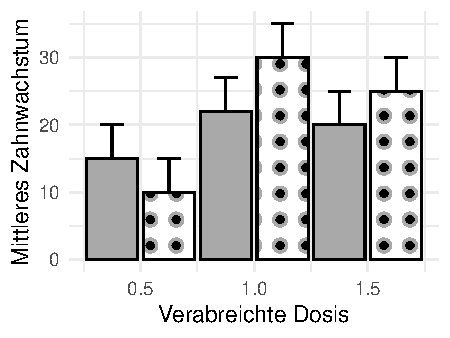
\includegraphics[width=\maxwidth]{img/mc-anova-02-a-1} 

}







\begin{enumerate}
\item [\textbf{A} \msquare] Die Koeffizienten sind positiv $(\beta_0 > 0; \beta_1 > 0)$.
\item [\textbf{B} \msquare] Keine Interaktion liegt vor $(p \leq 0.05)$.
\item [\textbf{C} \msquare] Das Bestimmtheitsmaß $R^2$ ist klein.
\item [\textbf{D} \msquare] Eine mittlere bis starke Interaktion liegt vor $(p \leq 0.05)$
\item [\textbf{E} \msquare] Die Koeffizienten sind negativ $(\beta_0 < 0; \beta_1 < 0)$.
\end{enumerate} 
\section*{Deskriptive Statistik \& Explorative Datenanalyse}

\section{Aufgabe \hfill (2 Punkte)}




Gegeben ist $y$ mit 14, 13, 5, 7 und 9. Berechnen Sie den Mittelwert und Standardabweichung.



\begin{enumerate}
\item [\textbf{A} \msquare] Sie erhalten 9.6 +/- 3.85
\item [\textbf{B} \msquare] Es ergibt sich 8.6 +/- 7.4
\item [\textbf{C} \msquare] Es berechnet sich 9.6 +/- 14.8
\item [\textbf{D} \msquare] Es berechnet sich 10.6 +/- 14.8
\item [\textbf{E} \msquare] Sie erhalten 9.6 +/- 1.925
\end{enumerate} 

\section{Aufgabe \hfill (2 Punkte)}




Berechnen Sie den Median, das $1^{st}$ Quartile sowie das $3^{rd}$ Quartile von $y$ mit 21, 18, 27, 13, 27, 26 und 42.




\begin{enumerate}
\item [\textbf{A} \msquare] Es berechnet sich 27 [19; 26]
\item [\textbf{B} \msquare] Sie erhalten 26 +/- 27
\item [\textbf{C} \msquare] Es ergibt sich 26 [18; 27]
\item [\textbf{D} \msquare] Sie erhalten 26 [16; 25]
\item [\textbf{E} \msquare] Es ergibt sich 26 +/- 18
\end{enumerate} 

\section{Aufgabe \hfill (2 Punkte)}



Mit einem Dotplot  können Sie sehr gut die Verteilung von Daten visualisieren. Die empfohlene Mindestanzahl an Beobachtungen ist dabei?



\begin{enumerate}
\item [\textbf{A} \msquare] 10 Beobachtungen.
\item [\textbf{B} \msquare] Damit wir hier sauber eine Abbilung von einem 
\item [\textbf{C} \msquare] Die opimale Anzahl ist größer als hundert Beobachtungen, wobei es gerne sehr viel mehr sein können.
\item [\textbf{D} \msquare] 2-5 Beobachtungen.
\item [\textbf{E} \msquare] Wir sollten eine Beobachtung mindestens pro Gruppe vorliegen haben.
\end{enumerate}

\section{Aufgabe \hfill (2 Punkte)}



Die Standardabweichung ist eine bedeutende deskriptive Statistik für die Analyse von Daten. Wie müssen Sie vorgehen um die Standardabweichung zu berechnen?



\begin{enumerate}
\item [\textbf{A} \msquare] Wir berechnen erst den Mittelwert und dann die absoluten Abstände zu dem Mittelwert. Diese quadratischen Abstände summieren wir auf und teilen am Ende durch die Fallzahl.
\item [\textbf{B} \msquare] Den Mittelwert berechen, dann die quadratischen Abstände zum Mittelwert aufsummieren und durch die Fallzahl teilen, dann die Wurzel ziehen.
\item [\textbf{C} \msquare] Wir berechnen erst den Mittelwert und dann die quadratischen Abstände zu dem Mittelwert. Diese quadratischen Abstände summieren wir auf und teilen am Ende durch die Fallzahl.
\item [\textbf{D} \msquare] Den Mittelwert berechnen und die Abstände quadrieren. Die Summe mit der Fallzahl multiplizieren.
\item [\textbf{E} \msquare] Den Mittelwert berechen, dann die absoluten Abstände zum Mittelwert aufsummieren
\end{enumerate} 

\section{Aufgabe \hfill (2 Punkte)}



Nachdem Sie eine ANOVA und die paarweisen t-Tests über das \Rlogo Paket \{emmeans\} durchgeführt haben, müssen Sie Ihre Daten nochmal zur Überprüfung visualisieren. Sie entscheiden sich für den Boxplot. Welche statistischen Maßzahlen stellt der Boxplot dar?

 



\begin{enumerate}
\item [\textbf{A} \msquare] Durch die Abbildung des Boxplot erhalten wir die Informationen über den Median und die Quartile.
\item [\textbf{B} \msquare] Der Boxplot stellt die Mittelwerte und die Standardabweichung dar.
\item [\textbf{C} \msquare] Der Boxplot stellt die Mittelwerte und die Varianz dar.
\item [\textbf{D} \msquare] Den Median und die Standardabweichung.
\item [\textbf{E} \msquare] Den Mittelwert und die Varianz.
\end{enumerate}

\section{Aufgabe \hfill (2 Punkte)}



In Ihrer Abschlussarbeit zuErbsen finden Sie aufeinmal seltsame Daten. Jedenfalls kommt Ihnen das so vor. Daher berechnen Sie den Mittelwert und den Median. Der Mittelwert $\bar{y}$ und der Median $\tilde{y}$ unterscheiden sich. Welche Aussage ist richtig?



\begin{enumerate}
\item [\textbf{A} \msquare] Wenn sich der Mittelwert und der Median unterscheiden, liegen vermutlich keine Outlier in den Daten vor.
\item [\textbf{B} \msquare] Der Mittelwert und der Median sollten gleich sein, wenn Outlier in den Daten vorliegen. 
\item [\textbf{C} \msquare] Da sich der Mittelwert und der Median unterscheiden, liegen vermutlich keine Outlier in den Daten vor. Wir verweden den Datensatz so wie er ist.
\item [\textbf{D} \msquare] Der Mittelwert und der Median sollten sich unterscheiden sein, wenn Outlier in den Daten vorliegen. 
\item [\textbf{E} \msquare] Da sich der Mittelwert und der Median unterscheiden, liegen vermutlich Outlier in den Daten vor. Wir untersuchen den Datensatz nach auffälligen Beobachtungen.
\end{enumerate}

\section{Aufgabe \hfill (2 Punkte)}



Sie wollen eine ANOVA im Anschluss an Ihr Feldexperiment rechnen. Dafür muss Ihr gemessener Endpunkt die Annahme einer Varianzhomogenität genügen. Zur Überprüfung können Sie folgende Visualisierung nutzen. Welche entsprechende Regel zur Abschätzung der Annahme einer Varianzhomogenität kommt zur Anwendung?



\begin{enumerate}
\item [\textbf{A} \msquare] Einen Barplot. Die Mittelwerte müssen alle auf einer Höhe liegen. Die Fehlerbalken haben hier keine Informationen.
\item [\textbf{B} \msquare] Einen Dotplot. Die Punkte müssen sich wie an einer Perlenschnurr audreihen. Eine Abweichung führt zur Ablehnung der Annahme einer Varianzhomogenität.
\item [\textbf{C} \msquare] Nach dem Einlesen der Daten nutzen wir einen Boxplot um zu schauen, ob alle Boxen über alle Behandlungen in etwa gleich groß sind. Damit ist dann auch das IQR in allen Behandlungen in etwa gleich.
\item [\textbf{D} \msquare] Einen Violinplot. Der Bauch der Violine muss hierbei einen höhren Wert annehmen als der Steg der Violine. Dann kann die Annahme einer Varianzhomogenität angenommen werden.
\item [\textbf{E} \msquare] In einer explorativen Datanalyse nutzen wir den Boxplot. Dabei sollte der Median als dicke Linie in der Mitte der Box liegen. Dann können wir von einer Varianzhomogenität ausgehen.
\end{enumerate}

\section{Aufgabe \hfill (2 Punkte)}




Sie wollen in Ihrer Abschlussarbeit über eine explorative Datenanalyse überprüfen, ob Ihr gemessener Endpunkt einer Normalverteilung folgt. Welche drei Abbildungen eignen sich insbesondere für die Überprüfung?





\begin{enumerate}
\item [\textbf{A} \msquare] Scatterplot, Mosaicplot, Boxplot
\item [\textbf{B} \msquare] Scatterplot, Densityplot, Barplot
\item [\textbf{C} \msquare] Violinplot, Boxplot, Densityplot
\item [\textbf{D} \msquare] Boxplot, Violinplot, Mosaicplot
\item [\textbf{E} \msquare] Histogramm, Scatterplot, Boxplot
\end{enumerate} 

\section{Aufgabe \hfill (2 Punkte)}



In dem folgenden Histogramm von $n = 218$ Pflanzen ist welche Verteilung abgebildet?



{\centering 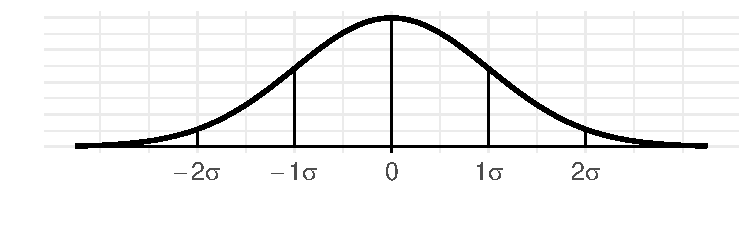
\includegraphics[width=\maxwidth]{img/mc-distribution-02-a-1} 

}







\begin{enumerate}
\item [\textbf{A} \msquare] Eine Standardnormalverteilung.
\item [\textbf{B} \msquare] Dem Histogramm entnehmen wir eine Possion-Verteilung.
\item [\textbf{C} \msquare] Es handelt sich um eine Binomial-Verteilung.
\item [\textbf{D} \msquare] In dem Histogramm ist eine Ordinalverteilung dargestellt.
\item [\textbf{E} \msquare] In dem Histogramm ist eine Normalverteilung dargestellt.
\end{enumerate} 
\section*{Lineare Regression \& Korrelation}

\section{Aufgabe \hfill (2 Punkte)}



Im Allgemeinen gibt es zwei mögliche Ziele für ein Regressionsmodell. Wir können eine Vorhersagemodell oder ein kausales Modell rechnen. Welche Aussage ist für ein prädiktives Modell richtig?



\begin{enumerate}
\item [\textbf{A} \msquare] Wenn ein prädiktives Modell gerechnet werden soll dann kann dies auf dem gesamten Datensatz geschehen. Das Ziel ist es einen Zusammenhang von $X$ auf $Y$ zu modellieren. Wie wirken sich die Einflussvariablen $Y$ auf die gemessenen Endpunkte $X = x_1, ..., x_p$ aus?
\item [\textbf{B} \msquare] Ein prädiktives Modell basiert auf einem Traingsdatensatz und einem Testdatensatz. Auf dem Trainingsdatensatz wird das Modell trainiert und auf dem Testdatensatz validiert.
\item [\textbf{C} \msquare] Ein prädiktives Modell möchte die Zusammenhänge von X auf Y modellieren. Hierbei geht es um die Effekte von $X$ auf $Y$. Man sagt, wenn $x_1$ um 1 ansteigt ändert sich $Y$ um einen Betrag $\beta_1$.
\item [\textbf{D} \msquare] Es wird ein Trainingsdatensatz zum Modellieren des Trainingsmodells benötigt. Der Testdatensatz dient rein zur Visualisierung. Dies gilt vor allem für ein prädiktives Modell.
\item [\textbf{E} \msquare] Ein prädiktives Modell benötigt mindestens eine Fallzahl von über 100 Beobachtungen und darf keine fehlenden Werte beinhalten. Die Varianzkomponenten müssen homogen sein.
\end{enumerate}

\section{Aufgabe \hfill (2 Punkte)}



Nach der Modellierung einer Regression stellt sich die Frage, ob die Residuen approximativ einer Normalverteilung folgen. Sie können einen QQ-Plot für die visuelle Überprüfung der Annahme an die Residuen nutzen. Welche Aussage ist richtig?



{\centering 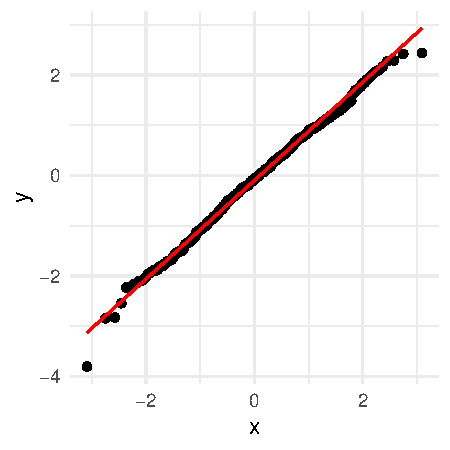
\includegraphics[width=\maxwidth]{img/mc-regression-05-a-1} 

}







\begin{enumerate}
\item [\textbf{A} \msquare] Wir betrachten die Punkte. Wenn die Punkte einigermaßen gleichmäßig verteilt liegen, dann gehen wir von normalen Residuen aus.
\item [\textbf{B} \msquare] Wir betrachten die Gerade. Wenn die Punkte einigermaßen gleichmäßig um die Gerade verteilt liegen, dann gehen wir von normalverteilten Residuen aus. Dies ist hier nicht der Fall. Wir haben keine normalverteilten Residuen vorliegen.
\item [\textbf{C} \msquare] Wir betrachten die Gerade und dabei insbesondere die beiden Enden der Gerade. Hier sollten die Punkte auf der Geraden liegen, dann ist die Annahme an die Normalverteilung der Residuen erfüllt.
\item [\textbf{D} \msquare] Die Annahme der normalverteilten Residuen ist erfüllt. Die Punkte liegen zum überwiegenden Teil nicht auf der Geraden.
\item [\textbf{E} \msquare] Die Annahme der normalverteilten Residuen ist nicht erfüllt. Die Punkte liegen zum überwiegenden Teil auf der Geraden.
\end{enumerate}

\section{Aufgabe \hfill (2 Punkte)}



Nach einer Regressions sollten die Residuen (\texttt{.resid}) gleichmäßig um die Gerade verortet sein. Was bei einer simplen Regression noch relativ einfach visuell in einem Scatterplot zu überprüfen ist. Für komplexere Modell liefert der Residual Plot die notwendigen Informationen. Welche Aussage ist richtig?



{\centering 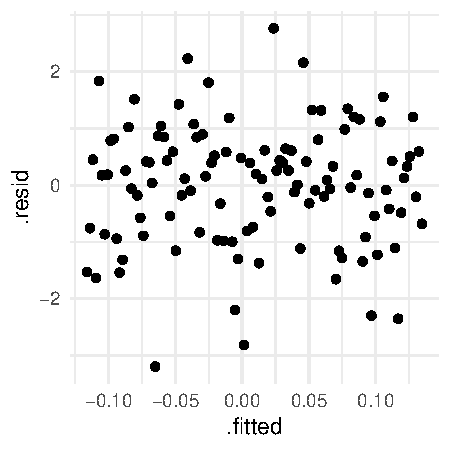
\includegraphics[width=\maxwidth]{img/mc-regression-06-a-1} 

}







\begin{enumerate}
\item [\textbf{A} \msquare] Wenn die Punkte gleichmäßig in dem positiven wie auch negativen Bereich ohne ein klares Muster liegen, dann hat unsere Modellierung geklappt. Wir können mit dem Modell weitermachen.
\item [\textbf{B} \msquare] Die Annahme der normalverteilten Residuen ist erfüllt. Die Punkte liegen zum überwiegenden Teil auf der Diagonalen. Damit ist das Modell erfolgreich geschätzt worden.
\item [\textbf{C} \msquare] Die Annahme der normalverteilten Residuen ist nicht erfüllt. Es ist kein Muster zu erkennen.
\item [\textbf{D} \msquare] Wenn wir die Nulllinie betrachten so müssen die Punkte gleichmäßig unter der Nulllinie liegen. Unser Modell erfüllt somit nicht die Annahme von normalverteilten Residuen mit einem Mittelwert von $>0$ und einer Streuung von $s$.
\item [\textbf{E} \msquare] Die Annahme der normalverteilten Residuen ist nicht erfüllt. Ein klares Muster ist zu erkennen und/oder einige Outlier sind zu beobachten.
\end{enumerate}

\section{Aufgabe \hfill (2 Punkte)}




Sie berechnen in Ihgrer Abschlussarbeit den Korrelationskoeffizienten $\rho$. Welche Aussage über den Korrelationskoeffizienten $\rho$ ist richtig?




\begin{enumerate}
\item [\textbf{A} \msquare] Korrelationskoeffizienten $\rho$ liegt zwischen 0 und 1. Darüber hinaus ist der Korrelationskoeffizienten $\rho$ einheitslos und kann als Standardisierung verstanden werden.
\item [\textbf{B} \msquare] Der Korrelationskoeffizienten $\rho$ liegt zwischen -1 und 1. Darüber hinaus ist der Korrelationskoeffizienten $\rho$ einheitslos und kann als standardisierte Steigung verstanden werden.
\item [\textbf{C} \msquare] Der Korrelationskoeffizienten $\rho$ liegt zwischen -1 und 1. Darüber hinaus ist der Korrelationskoeffizienten $\rho$ als standardisierte Steigung zu verstehen, wenn eine Standardisierung durchgeführt wurde. Diese Adjustierung nach Fischer muss am Anschluß der Berechnung der Korrelation durchgeführt werden.
\item [\textbf{D} \msquare] Der Korrelationskoeffizienten $\rho$ wird wie das $\eta^2$ aus der ANOVA interpretiert. Der Korrelationskoeffizienten $\rho$ beschreibt den Anteil an erklärter Varianz durch die Regression. Dabei gibt er jedoch eine Richtung an und kann auch negativ werden.
\item [\textbf{E} \msquare] Der Korrelationskoeffizienten $\rho$ ist eine standardisierte, statistische Maßzahl, die zwischen 0 und 1 liegt. Dabei ist Korrelationskoeffizienten $\rho$ einheitslos. Eine Signifikanz kann nicht nachgewiesen werden.
\end{enumerate}

\section{Aufgabe \hfill (2 Punkte)}



Nach einer simplen linearen Regression zur Untersuchung vom Einfluss der $NO_3$-Konzentration in [$\mu g$] im Wasser auf das Trockengewicht von Wasserlinsen in [$kg$] erhalten Sie einen $\beta_{NO_3}$ Koeffizienten von $6.9\times 10^{-7}$ und einen hoch signifikanten $p$-Wert mit $0.00051$. Warum sehen Sie so einen kleinen Effekt bei einer so deutlichen Signifikanz?




\begin{enumerate}
\item [\textbf{A} \msquare] Die Fallzahl ist zu hoch angesetzt. Je höher die Fallzahl ist, desto kleiner ist die Teststatistik und damit ist dann auch der $p$-Wert sehr klein. Es sollte über eine Reduzierung der Fallzahl nachgedacht werden. Dann sollte der Effekt zum p-Wert passen.
\item [\textbf{B} \msquare] Die Einheit der $NO_3$-Konzentration ist zu klein gewählt. Dadurch sehen wir den sehr kleinen $p$-Wert. Der $p$-Wert und die Einheit von der $NO_3$-Konzentration hängen antiproportional zusammen.
\item [\textbf{C} \msquare] Manchmal ist die Einheit der Einflussvariable $X$ zu klein gewählt, so dass der Ansteig von 1 Einheit in $X$ zu einer zu kleinen Änderung in $y$ führt. Daher kann der Effekt $\beta_{NO_3}$ sehr klein wirken, aber auf einer anderen Einheit sehr viel größer sein. Der p-Wert wird auf einer einheitslosen Teststatistik bestimmt.
\item [\textbf{D} \msquare] Wenn der Effekt $\beta_{NO_3}$ winzig ist, dann kann es an einer falsch gewählten Einheit liegen. Der Anstieg von einer Einheit in $X$ führt ja zu einer Änderung von $\beta_{NO_3}$ in $x$. Wir müssen daher die Einheit von $y$ entsprechend anpassen.
\item [\textbf{E} \msquare] Die Fallzahl ist zu klein angesetzt. Je kleiner die Fallzahl ist, desto höher ist die Teststatsitik und damit auch der $p$-Wert kleiner. Wir brauchen also mehr Fallzahl um den geringen Effekt noch signifikant zu krigen.
\end{enumerate}

\section{Aufgabe \hfill (2 Punkte)}



Nachdem Sie Ihr Experiment abgeschlossen haben, stehen Sie vor der Frage wie Sie Ihre Daten modellieren sollen. In der Beispielauswertung von Ihrem Betreuenden finden Sie die Funktion \texttt{lm()} in \Rlogo. Welche Aussage ist richtig?





\begin{enumerate}
\item [\textbf{A} \msquare] Ist die Einflussvariable $X$ numerisch so werden die Gruppenmittelwerte geschätzt und eine anschließende ANOVA sowie multipler Gruppenvergleich mit \{emmeans\} ist möglich.
\item [\textbf{B} \msquare] Die Funktion \texttt{lm()} in \Rlogo ist der letzte Schritt für einen Gruppenvergleich. Vorher kann eine ANOVA oder aber ein multipler Vergleich in \{emmeans\} gerechnet werden. In der Funktion  \texttt{lm()} werden die Gruppenvarianzen bestimmt.
\item [\textbf{C} \msquare] Die Funktion \texttt{lm()} in \Rlogo wird klassischerweise für die nicht-lineare Regression genutzt. Ist die Einflussvariable $X$ numerisch so werden die Gruppenmittelwerte geschätzt.
\item [\textbf{D} \msquare] Die Funktion \texttt{lm()} in \Rlogo wird klassischerweise für die lineare Regression genutzt. Ist die Einflussvariable $X$ ein Faktor so werden die Gruppenmittelwerte geschätzt und eine anschließende ANOVA sowie multipler Gruppenvergleich mit \{emmeans\} ist möglich.
\item [\textbf{E} \msquare] Neben der klassichen Verwendung der Funktion \texttt{lm()} in der linearen Regression kann auch ein Gruppenvergleich gerechnet werden. Dafür müssen aber alle Faktoren aus den Daten entfernt und numerishc umgewandelt werden. Dann kann das R Paket \{emmeans\} genutzt werden um die Korrelation zu berechnen. Eine Adjustierung ist dann nicht mehr notwendig.
\end{enumerate}

\section{Aufgabe \hfill (2 Punkte)}



Wenn Ihr gemessener Endpunkt nicht einer Normalverteilung folgt, so können Sie dennoch Ihre Daten modellieren. Hierzu nutzen Sie dann das \textit{generalisierte lineare Modell (GLM)}. Welche Aussage ist richtig?




\begin{enumerate}
\item [\textbf{A} \msquare] Das \textit{generalisierte lineare Modell (GLM)} erlaubt auch weitere Verteilungsgruppen für das $X$ bzw. die Einflussvariablen in einer linearen Regression zu wählen.
\item [\textbf{B} \msquare] Dank dem \textit{generalisierten linearen Modell (GLM)} können auch andere Verteilungsfamilien als die Normalverteilung mit einer linearen Regression modelliert werden.
\item [\textbf{C} \msquare] In \Rlogo ist mit dem \textit{generalisierten linearen Modell (GLM)} eine Modellierung implementiert, die die Poissonverteilung für Zähldaten oder die Binomialverteilung für 0/1-Daten modellieren kann. Weitere Modellierungen sind in \Rlogo auch mit zusätzlich geladenen Paketen nicht möglich.
\item [\textbf{D} \msquare] Das GLM ist ein faktisch maschineller Lernalgorithmus, der selstständig die Verteilungsfamilie für Y wählt.
\item [\textbf{E} \msquare] Das GLM ist eine Vereinfachung des LM in R. Mit dem GLM lassen sich polygonale Regressionen rechnen. Somit stehen neben der Normalverteilung noch weitere Verteilungen zu Verfügung.
\end{enumerate}
\section*{Vermischte Themen}  

\section{Aufgabe \hfill (2 Punkte)}

Die Randomisierung von Beobachtungen zu den Versuchseinheiten
ist bedeutend in der Versuchsplanung. Welche der folgenden Aussagen ist richtig?



\begin{enumerate}
\item [\textbf{A} \msquare] Randomisierung ist die direkte Folge von Strukturgleichheit. Die Strukturgleichheit erlaubt es erst von der Stichprobe auf die Grundgesamtheit zurückzuschliessen.
\item [\textbf{B} \msquare] Durch eine Randomisierung können wir nicht von Strukturgleichheit zwischen der Stichprobe und der Grundgesamtheit ausgehen.
\item [\textbf{C} \msquare] Strukturgleichheit ist durch Randomisierung gegeben. Leider hilft die Randomisierung noch nicht um von der Stichprobe auf die Grundgesamtheit zu schließen. Deshalb wurde das Falsifikationsprinzip entwickelt.
\item [\textbf{D} \msquare] Randomisierung sorgt für Strukturgleichheit und erlaubt erst von der Stichprobe auf die Grundgesamtheit zurückzuschliessen.
\item [\textbf{E} \msquare] Randomisierung bringt starke Unstrukturiertheit in das Experiment und erlaubt erst von der Stichprobe auf die Grundgesamtheit zurückzuschliessen.
\end{enumerate}

\section{Aufgabe \hfill (2 Punkte)}



Wenn Sie einen Datensatz erstellen, dann ist es ratsam die Spalten und die Einträge in englischer Sprache zu verfassen, wenn Sie später die Daten in \Rlogo auswerten wollen. Welcher Aussage ist richtig?



\begin{enumerate}
\item [\textbf{A} \msquare] Alle Funktionen und auch Anwendungen sind in \Rlogo in englischer Sprache. Die Nutzung von deutschen Wörtern ist nicht schick und das ist zu vermeiden.
\item [\textbf{B} \msquare] Es gibt keinen Grund nicht auch deutsche Wörter zu verwenden. Es ist ein Stilmittel.
\item [\textbf{C} \msquare] Programmiersprachen haben Probleme mit Umlauten und Sonderzeichen der deutschen Sprache. Daher ist die Nutzung in Deutsch in den AGBs von \Rlogo untersagt.
\item [\textbf{D} \msquare] Die Spracherkennung von \Rlogo ist nicht in der Lage Deutsch zu verstehen.
\item [\textbf{E} \msquare] Im Allgemeinen haben Programmiersprachen Probleme mit Umlauten und Sonderzeichen, die in der deutschen Sprache vorkommen. Eine Nutzung der englischen Sprache umgeht dieses Problem auf einfache Art.
\end{enumerate}

\section{Aufgabe \hfill (2 Punkte)}



Bei der explorativen Datenanalyse (EDA) in \Rlogo gibt es eine richtige Abfolge von Prozessschritten, auch 	extit{Circle of life} genannt. Wie lautet die richtige Reihenfolge für die Erstellung einer EDA?



\begin{enumerate}
\item [\textbf{A} \msquare] Wir lesen die Daten über eine generische Funktion \texttt{read()} ein und müssen dann die Funktion \texttt{ggplot()} nur noch installieren. Dann haben wir die Abbildungen als \texttt{*.png} vorliegen.
\item [\textbf{B} \msquare] Wir transformieren die Spalten über \texttt{mutate()} in ein \texttt{tibble} und können dann über \text{ggplot()} uns die Abbildungen erstellen lassen. Dabei beachten wir das wir keine Faktoren in den Daten haben.
\item [\textbf{C} \msquare] Wir lesen die Daten ein und mutieren die Daten. Dabei ist wichtig, dass wir nicht das Paket \texttt{tidyverse} nutzen, da dieses Paket veraltet ist. über die Funktion \texttt{library(tidyverse)} entfernen wir das Paket von der Analyse.
\item [\textbf{D} \msquare] Die Funktionsreihenfolge ist wie folgt: \texttt{read\_excel()} ->  \texttt{mutate()} -> \text{ggplot()}. Dabei ist bei der Transformation der Daten darauf zu achten, dass die Faktoren richtig erstellt werden.
\item [\textbf{E} \msquare] Für eine explorativen Datenanalyse (EDA) in \Rlogo müssen wir als erstes die Daten über \texttt{read\_excel()} einlesen. Danach müssen wir schauen, dass wir die Zeilen richtig über \texttt{mutate()} transformiert haben. Insbesondere müssen Variablen mit kontinuierlichen Werten in einen Faktor umgewandelt werden. Am Ende nutzen wir die Funktion \text{ggplot()} für die eigentlich EDA.
\end{enumerate}

\section{Aufgabe \hfill (2 Punkte)}



Sie haben das abstrakte Modell $Y \sim X$ mit $X$ als Faktor mit zwei Leveln vorliegen. Welche Aussage über $n_1 < n_2$ ist richtig?



\begin{enumerate}
\item [\textbf{A} \msquare] Es handelt sich um ein balanciertes Design.
\item [\textbf{B} \msquare] Es liegt Varianzhomogenität vor.
\item [\textbf{C} \msquare] Es liegt Varianzhetrogenität vor.
\item [\textbf{D} \msquare] Es handelt sich um ein unbalanciertes Design.
\item [\textbf{E} \msquare] Es handelt sich um abhängige Beobachtungen.
\end{enumerate}

\section{Aufgabe \hfill (2 Punkte)}



Die Leistung von Sauen soll auf einem Zuchtbetrieb gesteigert werden. Dafür werden die Ferkel verschiedener Sauen gemessen. Die Ferkel einer Muttersaue sind daher...



\begin{enumerate}
\item [\textbf{A} \msquare] Die Ferkel stammen von der gleichen Sau und sind somit untereinander abhängig.
\item [\textbf{B} \msquare] Untereinander stark korreliert. Die Ferkel sind von einer Mutter und sommit miteinander korreliert. Dies wird in der Statistik jedoch meist nicht modelliert.
\item [\textbf{C} \msquare] Je nach Stallanlage kommt eine andere Analyse in Betracht. Eine allgemeine Aussage über Ferkel und Sauen lässt sich statistisch nicht treffen.
\item [\textbf{D} \msquare] Untereinander unabhängig. Sollten die Mütter verwandt sein, so ist die Varianzstruktur ähnlich und muss modelliert werden.
\item [\textbf{E} \msquare] Abhängig von der Stallanlage und des Experiments können die Ferkel abhängig oder unabhängig sein. Allgmein gilt, dass Ferkel von unterschiedlichen Sauen näher miteinander verwandt sind als Ferkel von gleichen Sauen. Das Fisher-Axiom.
\end{enumerate}

\section{Aufgabe \hfill (2 Punkte)}



In einer Studie wollen Sie den Effektschätzer Risk ratio berechnen. Sie finden in Ihrem Experiment zur Behandlung von Klaueninfektionen bei Rinder in 6 Tieren Erkrankung der Klauen vor. 12 Tiere sind gesund. Welche Aussage ist richtig?



\begin{enumerate}
\item [\textbf{A} \msquare] Es ergibt sich ein Risk ratio von 0.5, da es sich um ein Anteil handelt.
\item [\textbf{B} \msquare] Der Anteil der Kranken wird berechnet. Da es sich um ein Anteil handelt ergibt sich ein Risk ratio von 0.33.
\item [\textbf{C} \msquare] Es ergibt sich ein Risk ratio von 0.33, da es sich um eine Chancenverhältnis handelt.
\item [\textbf{D} \msquare] Da es sich um ein Chancenverhältnis handelt ergibt sich ein Risk ratio von 3.
\item [\textbf{E} \msquare] Da es sich um ein Chancenverhältnis handelt ergibt sich ein Risk ratio von 0.5.
\end{enumerate}

\section{Aufgabe \hfill (2 Punkte)}



Sie werten in Ihrer Abschlussarbeit einen sehr großen Datensatz aus einer öffentlichen Datenbank aus. Nun stellen Sie fest, dass Sie ein Problem mit der Bewertung Ihrer Ergbnisse anhand der Signifikanz bekommen. Wie Sie herausfinden, scheint dies ein häufiges Problem in der Bio Data Science zu sein. Welche Aussage ist richtig?




\begin{enumerate}
\item [\textbf{A} \msquare] Eine erhöhte Fallzahl führt automatisch zu mehr signifikanten Ergebnissen auch wenn der Effekt klein ist und damit nicht relevant. Dadurch sind die Informationen zur Signifikanz in riesigen Datensätzen schwer zu verwerten, da fast alle Vergleiche signifikant sind.
\item [\textbf{B} \msquare] Big Data ist ein Problem der parametrischen Statistik. Parameter lassen sich nur auf kleinen Datensätzen berechnen, da es sich sonst nicht mehr um eine Stichprobe im engen Sinne der Statistik handelt.
\item [\textbf{C} \msquare] Aktuell werden immer größere Datensätze erhoben. Dadurch wird auch die Varianz immer höher was automatisch zu mehr signifikanten Ergebnissen führt.
\item [\textbf{D} \msquare] Riesige Datensätz haben mehr Fallzahl was zur $\alpha$-Inflation führt. Durch eine Adjustoerung kann dem Problem entgegengewirkt werden.
\item [\textbf{E} \msquare] Mehr Fallzahl in Datensätzen bedeutet mehr signifikante Ergebnisse, da in mehr Daten auch mehr Informationen beinhaltet sind. Deshalb lohnen sich riesige Datensätze, die durch die vielen signifikanten Ergebnisse auch eine Menge an relevanten Erkenntnissen liefern.
\end{enumerate}
\section*{Multiple Gruppenvergleiche}    

\section{Aufgabe \hfill (2 Punkte)}



Sie haben folgende unadjustierten p-Werte gegeben: 0.02, 0.34, 0.42, 0.01, 0.21 und 0.001. Sie adjustieren die p-Werte nach
Bonferroni. Welche Aussage ist richtig?



\begin{enumerate}
\item [\textbf{A} \msquare] Nach der Bonferroni-Adjustierung ergeben sich die adjustierten p-Werte von 0.12, 2.04, 2.52, 0.06, 1.26 und 0.006. Die adjustierten p-Werte werden zu einem $\alpha$-Niveau von 5\% verglichen.
\item [\textbf{B} \msquare] Nach der Bonferroni-Adjustierung ergeben sich die adjustierten p-Werte von 0.0033, 0.0567, 0.07, 0.0017, 0.035 und 2e-04. Die adjustierten p-Werte werden zu einem $\alpha$-Niveau von 0.83\% verglichen.
\item [\textbf{C} \msquare] Nach der Bonferroni-Adjustierung ergeben sich die adjustierten p-Werte von 0.12, 1, 1, 0.06, 1 und 0.006. Die adjustierten p-Werte werden zu einem $\alpha$-Niveau von 0.83\% verglichen.
\item [\textbf{D} \msquare] Nach der Bonferroni-Adjustierung ergeben sich die adjustierten p-Werte von 0.0033, 0.0567, 0.07, 0.0017, 0.035 und 2e-04. Die adjustierten p-Werte werden zu einem $\alpha$-Niveau von 5\% verglichen.
\item [\textbf{E} \msquare] Nach der Bonferroni-Adjustierung ergeben sich die adjustierten p-Werte von 0.12, 1, 1, 0.06, 1 und 0.006. Die adjustierten p-Werte werden zu einem $\alpha$-Niveau von 5\% verglichen.
\end{enumerate}

\section{Aufgabe \hfill (2 Punkte)}



Sie rechnen einen PostHoc-Test. Nun sollen Sie ein \textit{CLD} erstellen. Was bedeutet dieser Fachbegriff und welche folgende Beschreibung der Interpretation ist korrekt?



\begin{enumerate}
\item [\textbf{A} \msquare] Compound letter display. Gleichheit in dem Outcomes wird durch den gleichen Buchstaben oder Symbol dargestellt. Teilweise ist die Interpretation des Verbunds (eng. compound) herausfordernd, da wir ja nach dem Unterschied suchen.
\item [\textbf{B} \msquare] Compact letter display. Das CLD ist umstritten, da es die Gleichheit der Behandlungen durch gleiche Buchstaben darstellt. Dadurch ist das CLD nicht mehr sauber auf einer Linie mit dem statistischen Testen. Wir lehnen die Nullhypothese ab und zeigen keine Gleichheit im statistischen Testen.
\item [\textbf{C} \msquare] Compact line display. Gleichheit in den Behandlungen wird durch den gleichen Buchstaben oder Symbol dargestellt. Früher wurden keine Buchstaben sondern eine durchgezogene Linie verwendet. Bei mehr als drei Gruppen funktioniert die Linie aber graphisch nicht mehr.
\item [\textbf{D} \msquare] Compact letter display. Gleiche Buchstaben zeigen Gleichheit in den Behandlungen. Die Interpretation ist deshalb sehr intuitiv und einfach. Darüber hinaus ist damit das CLD auch auf einer Linie mit der Testtheorie, da wir ja auch dort die Gültigkeit der Nullhypothese nachweisen. Wir suchen ja Gleichheit.
\item [\textbf{E} \msquare] Contrast letter display. Unterschiede in den Behandlungen werden durch den gleichen Buchstaben oder Symbol dargestellt. Die Interpretation des CLD führt häufig in die Irre.
\end{enumerate}

\section{Aufgabe \hfill (2 Punkte)}




Der multiple Vergleich als Posthoc-Test nach einer ANOVA ist in den Agrarwissenschaften heutzutage Standard. Welches R Paket wird häufig für den multiplen Vergleich genutzt? Welche Beschreibung der Eigenschaften ist korrekt?



\begin{enumerate}
\item [\textbf{A} \msquare] Das R Paket \{emmeans\} erlaubt die Durchführung eines multiplen Gruppenvergleichs. Aus einem emmeans Objekt lässt sich leider kein CLD erstellen. Dennoch ist das Paket einfach zu bedienen und wird deshalb genutzt. Die Interpretation der statistischen Auswertung wird über einen Barplot abgebildet.
\item [\textbf{B} \msquare] Das R Paket \{lm\}. Das Paket \{lm\} erstellt selbstständig Konfidenzintervalle und entsprechende p-Werte. Da wir in dem Paket nicht adjustieren müssen, ist es bei Anwendern sehr beliebt.
\item [\textbf{C} \msquare] Das R Paket \{emmeans\} erlaubt die Durchführung eines multiplen Gruppenvergleichs. Aus einem \{emmeans\} Objekt lässt sich recht einfach das CLD erstellen und so über Barplots eine schnelle Interpration der statistischen Auswertung durchführen.
\item [\textbf{D} \msquare] Das R Paket \{hmisc\} erlaubt die Durchführung eines multiplen Gruppenvergleichs aus verschiedenen Modellen heraus. Aus einem hmisc Objekt lässt sich recht einfach das CLD erstellen und so über Barplots eine schnelle Interpration der statistischen Auswertung durchführen.
\item [\textbf{E} \msquare] Das R Paket \{ggplot\}. Wir erhalten hier sofort eine Visualisierung der Daten. Anhand der Visualisierung lässt sich eine explorative Datenanalyse durchführen, die gleichwertig zu einem Posthoc-Test ist.
\end{enumerate}

\section{Aufgabe \hfill (2 Punkte)}



In den Humanwissenschaften werden multiple Vergleiche häufig anders behandelt als in den Agrarwissenschaften. In beiden Bereichen tritt jedoch das gleiche Phänomen bei multiplen Testen auf. Wie muss mit dem Phänomen umgegangen werden und wie ist es benannt?



\begin{enumerate}
\item [\textbf{A} \msquare] Die Adjustierung der p-Werte nach Bonferroni erlaubt es gegen die $\beta$-Inflation vorzugehen, die häufig beim multiplen Testen auftritt. Das globale Powerniveau liegt nicht mehr bei $80\%$ sondern sehr viel niedriger.
\item [\textbf{B} \msquare] Beim multiplen Testen kann es zu einer $\alpha$-Inflation kommen. Das globale Signifikanzniveau liegt nicht mehr bei $5\%$ sondern sehr viel höher. Daher müssen die p-Werte entsprechend adjustiert werden. Hierfür gibt es verschiedene Verfahren, wobei das Verfahren zur Adjustierung der p-Werte nach Bonferroni das bekanneste Verfahren ist.
\item [\textbf{C} \msquare] Beim multiplen Testen kann es zu einer $\alpha$-Inflation kommen. Das globale Signifikanzniveau liegt nicht mehr bei $5\%$ sondern weit darunter. Daher müssen die p-Werte entsprechend adjustiert werden. Hierfür gibt es verschiedene Verfahren, wobei das Verfahren zur Adjustierung der p-Werte nach Welch das bekanneste Verfahren ist.
\item [\textbf{D} \msquare] Das globale Signifikanzniveau explodiert und erreicht Werte größer als Eins. Es kommt zu einer $\alpha$-Inflation. Dagegen kann mit der Adjustierung der $\alpha$-Werte nach Bonferroni vorgegangen werden.
\item [\textbf{E} \msquare] Das globale Signifikanzniveau liegt nicht mehr bei $5\%$ sondern sehr viel niedriger, bei ca. $1\%$. Es kommt zu einer $\alpha$-Hyperinflation. Dagegen kann mit der Adjustierung der p-Werte nach Bonferroni vorgegangen werden.
\end{enumerate}

\section{Aufgabe \hfill (2 Punkte)}




In einem Feldversuch haben Sie einen Behandlungsfaktor mit mehreren Leveln vorliegen. Sie rechnen einen multiplen Vergleich. Vorher hatten Sie eine einfaktorielle ANOVA mit einem signifikanten Ergebnis vorliegen. Welche Aussage ist richtig?



\begin{enumerate}
\item [\textbf{A} \msquare] Wenn ein multipler Test gerechnet wird, dann muss der Effekt $\Delta$ nicht adjustiert werden. Bei einem Effekt im multiplen Testen handelt es sich um eine Wahrscheinlichkeit für das Auftreten der Nullhypothese.
\item [\textbf{B} \msquare] Wenn ein multipler Test gerechnet wird, dann muss der Effekt $\Delta$ adjustiert werden im Gegensatz zu den p-Werten.
\item [\textbf{C} \msquare] Wenn ein multipler Test gerechnet wird, dann muss der Effekt $\Delta$ nicht adjustiert werden im Gegensatz zu den p-Werten.
\item [\textbf{D} \msquare] Beim multiplen Testen kann es zu einer Effektüberschätzung ($\Delta$-Inflation) kommen. Daher müssen die Effekte angepasst werden. Dies geschieht nicht händisch sondern intern in den angewendeten Algorithmen.
\item [\textbf{E} \msquare] Beim multiplen Testen werden die Effekte der paarweisen Vergleiche ignoriert. Der Nachteil des multiplen Testens ist ja auch, dass wir am Ende keine Effekte mehr vorliegen haben. Eine ANOVA liefert hier bessere Informationen.
\end{enumerate}
\section*{Statistische Testtheorie}  

\section{Aufgabe \hfill (2 Punkte)}




Sie haben den mathematischen Ausdruck $Pr(D|H_0)$ vorliegen, welche Aussage ist richtig?



\begin{enumerate}
\item [\textbf{A} \msquare] $Pr(D|H_0)$ ist die Wahrscheinlichkeit nicht die Daten $D$ zu beobachten sondern die Nullhypothese, wenn diese wahr ist.
\item [\textbf{B} \msquare] $Pr(D|H_0)$ stellt die Wahrscheinlichkeit die Teststatistik $T$ zu beobachten dar, wenn die Nullhypothese falsch ist.
\item [\textbf{C} \msquare] Die Wahrscheinlichkeit für die Nullhypothese, wenn die Daten wahr sind.
\item [\textbf{D} \msquare] $Pr(D|H_0)$ ist die Wahrscheinlichkeit der Alternativehypothese und somit $1 - Pr(H_A)$
\item [\textbf{E} \msquare] $Pr(D|H_0)$ stellt die Wahrscheinlichkeit die Daten $D$ und somit die Teststatistik $T_D$ zu beobachten dar, wenn die Nullhypothese wahr ist.
\end{enumerate}

\section{Aufgabe \hfill (2 Punkte)}



Die Testtheorie hat einen philosophischen Unterbau. Eins der Prinzipien ist das Falsifikationsprinzip. Das Falsifikationsprinzip besagt,



\begin{enumerate}
\item [\textbf{A} \msquare] ... dass Modelle meist falsch sind und selten richtig.
\item [\textbf{B} \msquare] ... dass in der Wissenschaft immer etwas falsch sein muss. Sonst gebe es keinen Fortschritt.
\item [\textbf{C} \msquare] ... dass ein schlechtes Modell durch ein schlechteres Modell ersetzt wird. Die Wissenschaft lehnt ab und verifiziert nicht.
\item [\textbf{D} \msquare] ... dass ein minderwertes Modell durch ein minderwertiges Modell ersetzt wird. Es gilt das Verifikationsprinzip nach Karl Popper.
\item [\textbf{E} \msquare] ... dass ein schlechtes Modell durch ein weniger schlechtes Modell ersetzt wird. Die Wissenschaft lehnt ab und verifiziert nicht.
\end{enumerate}

\section{Aufgabe \hfill (2 Punkte)}



In fast allen wissenschaftlichen Disziplinen liegt der Grenzwert für das Signifikanzniveau $\alpha$ bei 5\%. Wieso wurde dieser Konsens über die Signifikanzschwelle in dieser Form getroffen?



\begin{enumerate}
\item [\textbf{A} \msquare] Die Festlegung von $\alpha = 5\%$ ist eine Kulturkonstante. Wissenschaftler benötigt eine Schwelle für eine statistische Testentscheidung, der Wert von $\alpha$ wurde aber historisch mehr zufällig gewählt.
\item [\textbf{B} \msquare] Da Wissenschaftler eine Schwelle für die statistische Testentscheidung benötigen wurde $\alpha$ in einer großen Konferenz 1945 gewählt. Damit ist $\alpha = 5\%$ eine Kulturkonstante mit einem Rank einer Naturkonstante.
\item [\textbf{C} \msquare] Als Kulturkonstante hat $\alpha = 5\%$ den Rang einer Naturkonstante und wurde nach langer Diskussion in der UN im Jahre 1983 festgesetzt. Damals auch schon mit der Zustimmung der UdSSR.
\item [\textbf{D} \msquare] Der Begründer der modernen Statistik, R. Fischer, hat die Grenze simuliert und berechnet. Dadurch ergibt sich dieser optimale Cut-Off.
\item [\textbf{E} \msquare] Der Wert ergab sich aus einer Auswertung von 1042 wissenschaftlichen Veröffentlichungen zwischen 1914 und 1948. Der Wert $5\%$ wurde in $28\%$ der Veröffentlichungen genutzt. Daher legte man sich auf diese Zahl fest.
\end{enumerate}

\section{Aufgabe \hfill (2 Punkte)}

Betrachten wir die Teststatistik aus einem abstrakteren Blickwinkel. Beim
statistischen Testen wird das \textit{"`signal"'} mit dem
\textit{"`noise"'} aus den Daten $D$ zu einer Teststatistik $T_D$ verrechnet. Welche der Formel
berechnet korrekt die Teststatistik $T_D$?



\begin{enumerate}
\item [\textbf{A} \msquare] Es gilt $T_D = \cfrac{signal}{noise}$
\item [\textbf{B} \msquare] Es gilt $T_D = signal \cdot noise$
\item [\textbf{C} \msquare] Es gilt $T_D = \cfrac{noise}{signal}$
\item [\textbf{D} \msquare] Es gilt $T_D = (signal \cdot noise)^2$
\item [\textbf{E} \msquare] Es gilt $T_D = \cfrac{signal}{noise^2}$
\end{enumerate}

%% ------------------------------------------------------------

\section{Aufgabe \hfill (2 Punkte)}



Eine Analogie kann helfen einen Sachverhalt besser zu verstehen. Wie kann folgende Aussage richtig in die Analogie der statistischen Testtheorie gesetzt werden?

\begin{center}
\textit{$H_0$ beibehalten obwohl die $H_0$ falsch ist}
\end{center}



\begin{enumerate}
\item [\textbf{A} \msquare] Dem $\alpha$-Fehler in der Analogie eines Rauchmelder: \textit{Alarm without fire}.
\item [\textbf{B} \msquare] Dem $\beta$-Fehler mit der Analogie eines brennenden Hauses: \textit{Fire without alarm}.
\item [\textbf{C} \msquare] In die Analogie eines Rauchmelders: \textit{Fire without alarm}, dem $\beta$-Fehler.
\item [\textbf{D} \msquare] \textit{Alarm with fire}, dem $\alpha$-Fehler in der Analogie von Feuer.
\item [\textbf{E} \msquare] In die Analogie eines Feuerwehrautos: \textit{Car without noise}.
\end{enumerate}

\section{Aufgabe \hfill (2 Punkte)}



Sie lesen eine wissenschaftliche Arbeit, die damit wirbt, dass Effekte und Signifikanz nicht separat dargestellt sind, sondern in einer statistischen Maßzahl zusammen. Welche Aussage ist richtig?



\begin{enumerate}
\item [\textbf{A} \msquare] Das $\Delta$. Durch die Effektstärke haben wir einen Wert für die Relevanz, die vom Anwender bewertet werden muss. Da $\Delta$ antiproportional zum p-Wert ist, bedeutet auch ein hohes $\Delta$ ein sehr kleinen p-Wert.
\item [\textbf{B} \msquare] Über das Konfidenzintervall. Das Konfidenzinterval inkludiert eine Entscheidung über die Relevanz und zusätzlich kann über die Visualizierung des Konfidenzintervals eine Signifikanzschwelle vom Forschenden definiert werden.
\item [\textbf{C} \msquare] Das OR. Als Chancenverhältnis gibt es das Verhältnis von Relevanz und Signifikanz wieder.
\item [\textbf{D} \msquare] Das Konfidenzintervall. Durch die Visualizierung des Konfidenzintervals kann eine Relevanzschwelle vom Anwender definiert werden. Zusätzlich erlaubt das Konfidenzinterval auch eine Entscheidung über die Signifikanz.
\item [\textbf{E} \msquare] Die Teststatistik. Durch den Vergleich von $T_c$ zu $T_k$ ist es m{"o}glich die $H_0$ abzulehnen. Die Relevanz ergibt sich aus der Fläche rechts vom dem $T_c$-Wert.
\end{enumerate}

\section{Aufgabe \hfill (2 Punkte)}



Sie haben ein Signifikanzniveau $\alpha$ gleich 5\% vorliegen. Welche Aussage zusammen mit dem $p$-Wert ist richtig?



\begin{enumerate}
\item [\textbf{A} \msquare] Wir schauen, ob der $p$-Wert größer ist als das Signifikanzniveau $\alpha$ und vergleichen somit Wahrscheinlichkeiten. Die Wahrscheinlichkeiten werden als Flächen unter der Kurve der Teststaistik dargestellt, wenn die $H_A$ gilt.
\item [\textbf{B} \msquare] Wir machen ein Aussage über die Flächen und der Kurve der Teststatistik, wenn die $H_0$ gilt. Dabei werden Wahrscheinlichkeiten vergleichen, die durch die Flächen unter der Kurve repräsentiert werden.
\item [\textbf{C} \msquare] Wir vergleichen die Effekte des $p$-Wertes mit den Effekten der Signifikanzschwelle unter der Annahme der Nullhypothese. Dabei gilt, dass wir die Nullhypothese nur ablehnen können anhand des Falsifikationsprinzips.
\item [\textbf{D} \msquare] Wir vergleichen mit dem $p$-Wert und dem Signifikanzniveau $\alpha$ absolute Werte auf einem Zahlenstrahl und damit den Unterschied der Teststatistiken, wenn die $H_0$ gilt.
\item [\textbf{E} \msquare] Wir machen ein Aussage über die Flächen und zwischen den Kurve der Teststatistiken der Hypothesen $H_0$ und $H_A$, wenn die $H_0$ gilt. Dabei werden Wahrscheinlichkeiten vergleichen, die durch die Flächen unter der Kurve repräsentiert werden.
\end{enumerate}

\section{Aufgabe \hfill (2 Punkte)}



Um die Ergebnisse eines statistischen Tests und die damit verbundene Theorie besser zu verstehen, kann eine Analogie zur Wettervorhersage genutzt werden. Welche Analogie zu der Testtheorie trifft am meisten zu?



\begin{enumerate}
\item [\textbf{A} \msquare] In der Analogie der Sonnenscheindauer: Wie lange kann mit einem entsprechenden Effekt gerechnet werden? Die Wahrscheinlichkeit für den Effekt gibt der statistische Test wieder.
\item [\textbf{B} \msquare] In der Analogie des Niederschlags oder Regenmenge: ein statistischer Test gibt die Stärke eines Effektes wieder. Zum Beispiel, wie hoch ist der Mittelwertsunterschied.
\item [\textbf{C} \msquare] In der Analogie der Durchschnittstemperatur: Wie oft tritt ein Effekt durchschnittlich ein? Wir erhalten eine Wahrscheinlichkeit für die Effekte. Zum Beispiel, wie hoch ist die Wahrscheinlichkeit für einen Mittelwert als Durchschnitt.
\item [\textbf{D} \msquare] In der Analogie der Wahrscheinlichkeit für Regen: ein statistischer Test erlaubt die Wahrscheinlichkeit für ein Ereignis abzuschätzen. Die Stärke des Effektes können wir nicht bestimmen.
\item [\textbf{E} \msquare] In der Analogie der Regenwahrscheinlichkeit in einem bestimmten Gebiet: ein statistischer Test gibt die Wahrscheinlichkeit für ein Ereignis in einem Experiment mit den Daten $D$ wieder und lässt sich kaum verallgemeinern.
\end{enumerate}

\section{Aufgabe \hfill (2 Punkte)}



In Ihrer Forschungsarbeit wollen Sie eine Aussage über die untersuchte Population treffen. Dazu nutzen Sie eine ANOVA als statistischen Test. Erhalten Sie eine valide Aussage aus einem statistischen Test?



\begin{enumerate}
\item [\textbf{A} \msquare] Ja, wir können die untersuchte Population nicht mit einer ANOVA auswerten. Wir erhalten keine Aussage zur Population. Wir können aber den Test adjustieren und so die Auswertung ermöglichen.
\item [\textbf{B} \msquare] Nein, wir können die untersuchte Population nicht mit einem t-Test auswerten. Wir erhalten keine Aussage zur Population. Wir können aber den Effekt als Quelle der Relevanz nutzen.
\item [\textbf{C} \msquare] Nein, es ist nicht möglich die untersuchte Population mit einem t-Test auszuwerten. Wir erhalten dann leider keine Aussage zur Population.
\item [\textbf{D} \msquare] Ja, es ist möglich die untersuchte Population mit einem t-Test auszuwerten. Wir erhalten dann eine Aussage zur Population.
\item [\textbf{E} \msquare] Weder eine Ausssage über die Population noch über das Individuum ist mit einem statistischen Test möglich. Wir erhalten eine Aussage über ein Experiment.
\end{enumerate}

\section{Aufgabe \hfill (2 Punkte)}



Sie haben die \textit{Power} berechnet. Was sagt Ihnen dieser statistische Begriff aus?



\begin{enumerate}
\item [\textbf{A} \msquare] Alle statistischen Tests sind so konstruiert, dass die $H_A$ mit 20\% \textit{bewiesen wird}. Die Power ist $1-\beta$ mit $\beta$ gleich 80\% gesetzt.
\item [\textbf{B} \msquare] Die Power $1-\beta$ wird auf 80\% gesetzt. Damit liegt die Wahrscheinlichkeit für die $H_0$ bei 20\%.
\item [\textbf{C} \msquare] Die Power wird nicht berechnet sondern ist eine Eigenschaft des Tests. Die Power wird auf $80\%$ gesetzt und beschreibt mit welcher Wahrscheinlichkeit $H_A$ \textit{bewiesen wird}
\item [\textbf{D} \msquare] Die Power ist nicht in der aktuellen Testthorie mehr vertreten. Wir rechnen nur noch mit dem Fehler 1. Art.
\item [\textbf{E} \msquare] Die Power beschreibt die Wahrscheinlichkeit die $H_A$ abzulehnen. Wir testen die Power jedoch nicht.
\end{enumerate}

\section{Aufgabe \hfill (2 Punkte)}



Sie rechnen einen statistischen Test und erhalten neben dem p-Wert noch einen Effekt wiedergegeben. Welche Aussage zum Effekt ist richtig?



\begin{enumerate}
\item [\textbf{A} \msquare] Der Effekt eines statistischen Tests beschreibt die mathematisch interpretierbare Ausgabe eines Tests. Damit ist der Effekt direkt mit dem Begriff der Signifikanz verbunden. Die Entscheidung über die Signifikanz trifft der Forschende unabhängig von der Relevanz eines statistsichen Tests.
\item [\textbf{B} \msquare] Der Forschende muss am Ende wissen, ob das Eregbnis eines Experiments relevant für seine Forschung ist. Dafür kann der Effekt eines statistischen Tests genutzt werden. Damit beschreibt der Effekt den biologischen interpretierbaren Teil einer Ausgabe eines Tests. Zum Beispiel der Unterschied zwischen zwei Anteilen.
\item [\textbf{C} \msquare] Der Effekt eines statistischen Tests beschreibt die biologisch interpretierbare Ausgabe eines Tests. Damit ist der Effekt direkt mit dem Begriff der Signifikanz verbunden. Die Entscheidung über die Signifikanz trifft der Forschende unabhängig von der Relevanz eines statistsichen Tests.
\item [\textbf{D} \msquare] Der Forschende muss am Anfang wissen, ob das Eregbnis eines Experiments relevant für seine Forschung ist. Dafür kann der Effekt eines statistischen Tests genutzt werden oder auch der Prähoc-Test. Damit beschreibt der Effekt den biologischen interpretierbaren Teil eines Experimnts vor der Durchführung. Zum Beispiel der Unterschied zwischen zwei Mittelwerten.
\item [\textbf{E} \msquare] Der Effekt eines statistischen Tests beschreibt die biologisch interpretierbare Ausgabe eines Tests. Moderen Algorithmen liefern keine Effekte mehr sondern nur noch bedingte Wahrscheinlichkeiten. Der Effekt spielt in der modernen Statistik keine Rollen mehr.
\end{enumerate}

\section{Aufgabe \hfill (2 Punkte)}



Welche Aussage über die Entscheidung anhand des p-Wertes gegen die
Nullhypothese ist richtig?



\begin{enumerate}
\item [\textbf{A} \msquare] Anhand des p-Wertes lässt sich wie folgt eine Entscheidung treffen. Liegt der Wert in dem Signifikanzniveauintervall $\alpha$ dann kann die Nullhypothese abgelehnt werden.
\item [\textbf{B} \msquare] Ist $T_{D}$ h{"o}her als der kritische Wert $T_{\alpha = 5\%}$ dann wird die Nullhypothese $H_0$ abgelehnt.
\item [\textbf{C} \msquare] Ist $Pr(D|H_0)$ kleiner als das Signifikanzniveau $\alpha$ gleich $5\%$ dann wird die Nullhypothese $H_0$ abgelehnt.
\item [\textbf{D} \msquare] Anhand des p-Wertes lässt sich wie folgt eine Entscheidung treffen. Liegt der Wert über oder gleich dem Signifikanzniveau $\alpha$ dann kann die Nullhypothese abgelehnt werden.
\item [\textbf{E} \msquare] Ist in dem 95\%-Konfidenzintervall nicht die Null enthalten dann wird die Nullhypothese $H_0$ abgelehnt.
\end{enumerate}

\section{Aufgabe \hfill (2 Punkte)}



In Ihrer Abschlussarbeit müssen Sie für die statistischen Tests im Anhang Ihrer Arbeit die Hypothesen $H$ formulieren. Welche Aussage über Hypothesen $H$ ist richtig



\begin{enumerate}
\item [\textbf{A} \msquare] Es gibt ein Hypothesenset bestehend aus $k$ Hypothesen. Meistens wird die Nullhypothese $H_0$ und die Alternativhypothese $H_A$ verwendet. Wegen des Falsifikationsprinzips ist es wichtig, die bekannte falsche und unbekannte richtige Hypothese mit in das Set zu nehmen.
\item [\textbf{B} \msquare] Ein statistisches Hypothesenpaare gibt es. Zum einen die Nullhypothese $H_0$ und zum anderen die Alternativehypothese $H_A$ oder $H_1$
\item [\textbf{C} \msquare] Es gibt ein statistisches Hypothesenpaar mit der Hypothese für und gegen die wissenschaftliche Fragestellung. Die Hypothesen werden $H_{pro}$ und $H_{contra}$ bezeichnet.
\item [\textbf{D} \msquare] Ein statistisches Hypothesenpaare gibt es. Zum einen die Nullhypothese und zum anderen die Alternativehypothese. Es ist aber nur notwendig die Alternative anzugeben, da die Nullhypothese nicht beim Testen benötigt wird.
\item [\textbf{E} \msquare] Mit der Nullhypothese $H_A$ und der Alternativehypothese $H_0$ gibt es zwei Hypothesen, die aber selten genutzt werden.
\end{enumerate}
\section*{Statistische Tests für Gruppenvergleiche} 

\section{Aufgabe \hfill (2 Punkte)}



Nach einem Feldexperiment wollen Sie zwei Gruppen mit einem Welch t-Test vergleichen. Welche Aussage ist auch für den Student t-Test richtig?



\begin{enumerate}
\item [\textbf{A} \msquare] Der t-Test ist ein Vortest der ANOVA und basiert daher auf dem Vergleich von Streuungsparametern
\item [\textbf{B} \msquare] Der t-Test berechnet die Differenz von zwei Mittelwerten als Effekt und gibt eine Entscheidung, ob sich die beiden Mittelwerte \textit{jeweils} von Null unterscheiden.
\item [\textbf{C} \msquare] Der t-Test vergleicht zwei oder mehr Gruppen indem die Mittelwerte miteinander verglichen werden.
\item [\textbf{D} \msquare] Der t-Test vergleicht die Mittelwerte von zwei Gruppen unter der strikten Annahme von Varianzhomogenität. Sollte keine Varianzhomogenität vorliegen, so gibt es keine Möglichkeit den t-Test in einer Variante anzuwenden.
\item [\textbf{E} \msquare] Der t-Test vergleicht die Mittelwerte von zwei Gruppen.
\end{enumerate}

\section{Aufgabe \hfill (2 Punkte)}



Ein Versuch wurde in 10 Parzellen pro Gruppe durchgeführt. Die folgende Abbildung enthält die Daten aus diesem Versuch zur Bewertung der Wirkung des Mikronährstoff Nitrat auf den Ertrag in t/ha von Weizen im Vergleich zu einer Kontrolle.  Welche Aussage ist richtig, wenn Sie einen t-Test rechnen?



{\centering 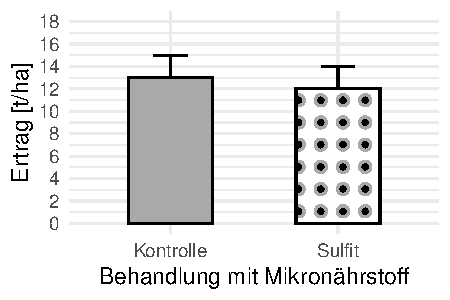
\includegraphics[width=\maxwidth]{img/mc-testing-ttest-02-1} 

}







\begin{enumerate}
\item [\textbf{A} \msquare] Der Effekt und die Signifikanz lassen sich nicht aus Barplots abschätzen. Höchtens der Effekt als relativer Unterschied zwischen der Höhe der Barplots. Standard ist der mediane Unterschied aus Boxplots.
\item [\textbf{B} \msquare] Es liegt kein signifikanter Unterschied vor. Der Effekt liegt bei 10.
\item [\textbf{C} \msquare] Der Test deutet auf einen signifikanten Unterschied hin. Der Effekt liegt vermutlich bei 10.
\item [\textbf{D} \msquare] Es liegt ein signifikanter Unterschied vor. Der Effekt liegt bei 1.
\item [\textbf{E} \msquare] Die Barplots deuten auf einen signifikanten Unterschied. Der Effekt liegt vermutlich bei 10 unter einer groben Abschätzung. Wir müssen aber eine ANOVA rechnen um den Effekt wirklich bestimmen zu können.
\end{enumerate}

\section{Aufgabe \hfill (2 Punkte)}




Welche Aussage über den gepaarten t-Test für verbundene Stichproben ist richtig?



\begin{enumerate}
\item [\textbf{A} \msquare] Der gepaarte t-Test wird gerechnet, wenn die Beobachtungen nicht unabhängig voneinander sind. Wir messen wiederholt an dem gleichen Probanden oder Tier oder Pflanze. Wir bilden die Differenzen um den gepaarten t-Test rechnen zu können.
\item [\textbf{B} \msquare] Der gepaarte t-Test wird gerechnet, wenn die Beobachtungen abhängig voneinander sind. Wir messen jede Beobachtung nur einmal und berechnen dann die Differenz zu dem Mittel der anderen Beobachtungen.
\item [\textbf{C} \msquare] Der gepaarte t-Test wird genutzt, wenn die Differenzen der Beobachtungen verbunden sind und wir dadurch die Unabhäängigkeit nicht mehr vorliegen haben.
\item [\textbf{D} \msquare] Der gepaarte t-Test nutzt die Varianz der Beobachtungen jeweils paarweise und bildet dafür eine verbundene Stichprobe. Dieser Datensatz $d$ dient dann zur Differenzbildung.
\item [\textbf{E} \msquare] Beim gepaarten t-Test kombinieren wir die Vorteile des Student t-Test für Varianzhomogenität mit den Vorteilen des Welch t-Test für Varianzheterogenität. Wir bilden dafür die Differenz der Einzelbeobachtungen.
\end{enumerate}

\section{Aufgabe \hfill (2 Punkte)}



In Ihrer Abschlussarbeit passen die Ergebnisse einer ANOVA und eines multiplen Vergleiches nicht zusammen. Nach einem Experiment mit vier Maissorten ergibt eine ANOVA ($p = 0.048$). Sie führen anschließend die paarweisen t-Tests für alle Vergleiche durch. Nach der Adjustierung für multiples Testen ist kein p-Wert unter der $\alpha$-Schwelle. Sie schauen sich auch die rohen, unadjustierten p-Werte an und finden hier als niedrigsten p-Wert $p_{3-2} = 0.052$. Welche Aussage ist richtig?




\begin{enumerate}
\item [\textbf{A} \msquare] Hier kommt der Effekt der stiegenden Fallzahl auf die Anzahl an signifikante Ergebnisse zu tragen. Da die ANOVA auf weniger Fallzahl testet als die paarweisen t-Tests, kann die ANOVA schwerer einen signifikanten Unterscheid nachweisen.
\item [\textbf{B} \msquare] Das ist kein Wunder. Die ANOVA testet auf der gesamten Fallzahl und die paarweisen t-Tests verlieren immer eine oder mehr Gruppen als Fallzahl. Mit steigender Fallzahl sind mehr signifikante Unterschiede zu erwarten. Die p-Werte unterscheiden sich numerisch auch kaum.
\item [\textbf{C} \msquare] Das Beispiel kann so nicht auftreten, da die ANOVA und die t-Tests algorithmisch miteinander verschränkt sind.
\item [\textbf{D} \msquare] Es gibt einen Fehler in der Varianzstruktur. Daher kann die ANOVA nicht richtig sein und paarweise t-Tests liefern das richtige Ergebnis.
\item [\textbf{E} \msquare] Die ANOVA testet auf der gesamten Fallzahl. Es wäre besser die ANOVA auf der gleichen Fallzahl wie die einzelnen t-Tests zu rechnen.
\end{enumerate}
    
% -----------------------------------------------------------------------
\clearpage
% -----------------------------------------------------------------------
\part{Deskriptive Statistik \& Explorative Datenanalyse}
% -----------------------------------------------------------------------

\section{Aufgabe \hfill (8 Punkte)}

\textit{Geben Sie grundsätzlich Formeln und Rechenweg zur Lösung der Teilaufgaben mit an!} \\[1Ex]
 

 
%% --------------------------------------------------------------------
\begin{minipage}[t]{0.5\textwidth}

\includegraphics[width = 1.3cm]{/Users/kruppajo/work/GitHub/exam/avatare/Alex.png}
\end{minipage}
\begin{minipage}[t]{0.5\textwidth}
\hfill
\href{https://youtu.be/t0WYa_LVc5o}{
\includegraphics[width = 2cm]{img/youtube}}
\end{minipage}
\vspace{-3ex}
%% --------------------------------------------------------------------



\paragraph{Zerforschen des Barplots}

Barplots sind bedeutend in der Darstellung von wissenschaftlichen Ergebnissen. Leider hat sich Alex nicht gemerkt, welche statistischen Maßzahlen für einen Barplot erhoben werden müssen. Besser wäre was anderes gewesen. Starcraft. Ein wunderbares Hobby um sich drin zu verlieren und Abstand zu bekommen. Alex denkt gerne über Starcraft nach. Das ist in soweit doof, da nach seiner Betreuer erstmal ein Barplot nachgebaut werden soll, bevor es mit seiner Hausarbeit losgeht. Dann hat er schonmal den \Rlogo Code vorliegen und nachher geht dann alles schneller. Na dann mal los. Alex schafft sich die nötige Stimmung. Alex streichelt liebevoll die Katze. Der Kopf ist in seinem Schloß vergraben um den Klang von Abba zu dämpfen. In der Behandlung für Maiss werden verschiedene Düngestufen ($ctrl$, $low$ und $high$) sein. Erfasst wird als Messwert ($Y$) \textit{Frischegewicht}. Alex soll dann \textit{freshmatter} in seiner Exceldatei eintragen.



{\centering 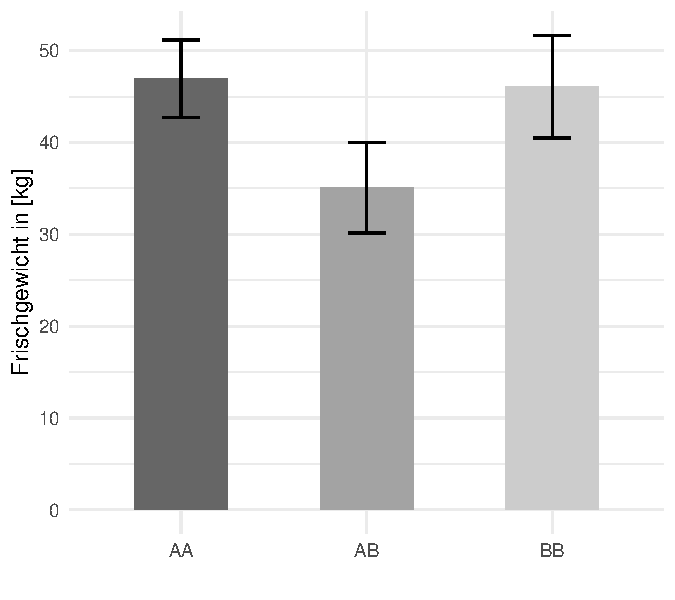
\includegraphics[width=\maxwidth]{img/barplot-02-1} 

}




Leider kennt sich Alex mit der Erstellung von Barplots in \Rlogo nicht aus. Deshalb braucht er bei der Visualisierung Ihre Hilfe!

\begin{enumerate}
\item Formulieren Sie die wissenschaftliche Fragestellung! \textbf{(1 Punkt)}
\item Erstellen Sie eine Tabelle mit den statistischen Maßzahlen der drei Barplots! \textit{Beachten Sie die korrekte Darstellungsform der statistischen Maßzahlen!} \textbf{(3 Punkte)}
\item Erstellen Sie einen beispielhaften Datensatz im \Rlogo üblichen Format, aus dem die drei Barplots \textit{möglicherweise} erstellt wurden! \textbf{(2 Punkte)}
\item Kann Alex einen Unterschied zwischen den Behandlungen erwarten? Begründen Sie Ihre Antwort! \textbf{(2 Punkte)}
\end{enumerate} 
\clearpage
% -----------------------------------------------------------------------

\section{Aufgabe \hfill (8 Punkte)}

\textit{Geben Sie grundsätzlich Formeln und Rechenweg zur Lösung der Teilaufgaben mit an!} \\[1Ex]
 

 
%% --------------------------------------------------------------------
\begin{minipage}[t]{0.5\textwidth}

\includegraphics[width = 1.3cm]{/Users/kruppajo/work/GitHub/exam/avatare/Jonas.png}
\end{minipage}
\begin{minipage}[t]{0.5\textwidth}
\hfill
\href{https://youtu.be/vXnLttRL_VI}{
\includegraphics[width = 2cm]{img/youtube}}
\end{minipage}
\vspace{-3ex}
%% --------------------------------------------------------------------



\paragraph{Visualisierung des Barplots}


Barplots sind bedeutend in der Darstellung von wissenschaftlichen Ergebnissen. Leider hat sich Jonas nicht gemerkt, welche statistischen Maßzahlen für einen Barplot erhoben werden müssen. Besser wäre was anderes gewesen. Jonas liebt Stricken. Darin kann er sich wirklich verlieren und immer wieder neu begeistern. Das ist in soweit doof, da nach seinem Betreuer nun Barplots aus seinen Daten gebaut werden sollen, bevor es mit dem statistischen Testen weitergeht. Na dann mal los. Jonas schafft sich die nötige Stimmung. Jonas nickt im Takt von Iron Maiden und bemerkt dabei gar nicht was das Meerschweinchen schon wieder anstellt. Die Behandlung für Brokoli waren verschiedene Bewässerungstypen ($low$, $mid$ und $high$). Erfasst wurde von Jonas als Messwert ($Y$) \textit{Trockengewicht}. Jonas hat dann \textit{drymatter} in seiner Exceldatei eintragen. Aber auch irgendwie egal. Jonas will später nochmal raus um zu Schwimmen. Druck ablassen, dass muss er auch.

\begin{table}[!h]
\centering
\begin{tabular}{cc}
\toprule
treatment & drymatter\\
\midrule
mid & 21.5\\
mid & 32.4\\
high & 28.6\\
high & 31.6\\
mid & 25.5\\
\addlinespace
low & 33.8\\
mid & 29.8\\
low & 26.6\\
high & 23.2\\
low & 27.3\\
\addlinespace
mid & 27.4\\
\bottomrule
\end{tabular}
\end{table}



Leider kennt sich Jonas mit der Erstellung von Barplots nicht aus. Deshalb braucht er bei der Visualisierung Ihre Hilfe!

\begin{enumerate}
\item Formulieren Sie die wissenschaftliche Fragestellung! \textbf{(1 Punkt)}
\item Zeichnen Sie in \textit{einer} Abbildung die Barplots für die Behandlung von Brokoli! Beschriften Sie die Achsen entsprechend!\textbf{(4 Punkte)}
\item Beschriften Sie \textit{einen} Barplot mit den gängigen statistischen Maßzahlen! \textbf{(2 Punkte)}
\item Wenn Jonas \textit{keinen Effekt} zwischen den Behandlungen von Brokoli erwarten würde, wie sehen dann die Barplots aus? \textit{Antworten Sie mit einer Skizze der Barplots!}
  \textbf{(1 Punkt)}
\end{enumerate} 
\clearpage
% -----------------------------------------------------------------------

\section{Aufgabe \hfill (9 Punkte)}

\textit{Geben Sie grundsätzlich Formeln und Rechenweg zur Lösung der Teilaufgaben mit an!} \\[1Ex]
 

 
%% --------------------------------------------------------------------
\begin{minipage}[t]{0.5\textwidth}

\includegraphics[width = 1.3cm]{/Users/kruppajo/work/GitHub/exam/avatare/Nilufar.png}
\end{minipage}
\begin{minipage}[t]{0.5\textwidth}
\hfill
\href{https://youtu.be/Xf0yE-o7bEU}{
\includegraphics[width = 2cm]{img/youtube}}
\end{minipage}
\vspace{-3ex}
%% --------------------------------------------------------------------



\paragraph{Zerforschen des Boxplots}

Wenn die Erwartung nicht wäre, ja dann wäre wohl vieles möglich für Nilufar! Aber so.. Deshalb gilt anschauen, was andere vor einem gemacht haben. Für Nilufar ist es eine Möglichkeit schneller ans Ziel zu gelangen. Nilufar soll in ihrer Hausarbeit Lauch untersuchen. Die Behandlung in ihrer Hausarbeit werden verschiedene Lichtstufen ($none$, $200lm$ und $600lm$) sein. Erheben wird Nilufar als Messwert ($Y$) \textit{Trockengewicht} benannt als \textit{drymatter} in ihrer Exceldatei. Von ihrer Betreuerin erhält sie nun folgende Abbildung von Boxplots, die sie erstmal zur Übung nachbauen soll, bevor sie mit dem eigentlichen Versuch beginnt. Aber nur in passender Atmospäre! Auf seinem Second Screen läuft Star Trek und Nilufar schaufelt Takis Blue Heat. Nicht effizient, aber gut.



{\centering 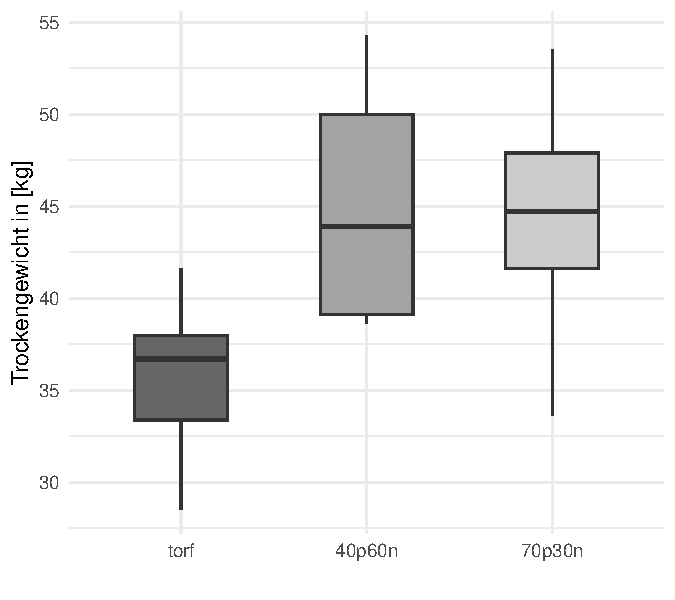
\includegraphics[width=\maxwidth]{img/boxplot-02-zer-1} 

}




Leider kennt sich Nilufar mit der Erstellung von Boxplots in \Rlogo nicht aus. Deshalb braucht sie bei der Visualisierung Ihre Hilfe!

\begin{enumerate}
\item Erstellen Sie eine Tabelle mit den statistischen Maßzahlen aus der obigen Abbildung der drei Boxplots! \textit{Beachten Sie die korrekte Darstellungsform der statistischen Maßzahlen!} \textbf{(3 Punkte)}
\item Beschriften Sie \textit{einen} der Boxplots mit den gängigen statistischen Maßzahlen! \textbf{(2 Punkte)}
\item Erstellen Sie einen beispielhaften Datensatz, aus dem die drei Boxplots \textit{möglicherweise} erstellt wurden, im \Rlogo üblichen Format! \textbf{(2 Punkte)}
\item Kann Nilufar einen Unterschied zwischen den Behandlungen erwarten? Begründen Sie Ihre Antwort! \textbf{(2 Punkte)}
\end{enumerate} 
\clearpage
% -----------------------------------------------------------------------

\section{Aufgabe \hfill (9 Punkte)}

\textit{Geben Sie grundsätzlich Formeln und Rechenweg zur Lösung der Teilaufgaben mit an!} \\[1Ex]
 

 
%% --------------------------------------------------------------------
\begin{minipage}[t]{0.5\textwidth}

\includegraphics[width = 1.3cm]{/Users/kruppajo/work/GitHub/exam/avatare/Paula.png}
\end{minipage}
\begin{minipage}[t]{0.5\textwidth}
\hfill
\href{https://youtu.be/0xc0jIPeiyw}{
\includegraphics[width = 2cm]{img/youtube}}
\end{minipage}
\vspace{-3ex}
%% --------------------------------------------------------------------



\paragraph{Visualisierung des Boxplots}

Eine echte Herausforderung für sie war schon immer der Perfektionismus gewesen. Ein leidiges Lied. Deshalb gilt anschauen, was andere vor einem gemacht haben. Für Paula ist es eine Möglichkeit schneller ans Ziel zu gelangen. Deshalb hat sich Paula viele Poster in der Fakultät angeschaut und ist zum Schluß gekommen, dass Boxplots eine häufig genutzte Abbildung sind. Paula soll nun in ihrer Hausarbeit Kartoffeln untersuchen. Die Behandlung in ihrer Hausarbeit sind verschiedene Bewässerungstypen ($low$ und $high$). Erhoben wurden von Paula als Messwert ($Y$) \textit{Frischegewicht} benannt als \textit{freshmatter} in ihrer Exceldatei. Erwartungsgemäß erhält sie von ihrer Betreuerin den Auftrag die erhobenen Daten als Boxplots darzustellen. Dann kann Paula auch schonmal abschätzen, was bei einem statistischen Test rauskommen könnte. Darüber hinaus kann Paula anhand Boxplots eine Aussage über die Varianzhomogenität über die Behandlungsgruppen treffen. Na dann mal los. Paula schafft sich die nötige Stimmung. Paula nickt im Takt von White Lies und bemerkt dabei gar nicht was die Ratte schon wieder anstellt.

\begin{table}[!h]
\centering
\begin{tabular}{cc}
\toprule
treatment & drymatter\\
\midrule
low & 40.0\\
high & 24.7\\
low & 41.7\\
low & 41.0\\
low & 43.1\\
\addlinespace
low & 41.0\\
high & 20.0\\
low & 44.7\\
low & 39.3\\
high & 31.8\\
\addlinespace
high & 20.4\\
high & 25.2\\
low & 35.6\\
low & 39.1\\
high & 25.9\\
\addlinespace
low & 39.3\\
high & 23.4\\
high & 13.0\\
high & 24.2\\
\bottomrule
\end{tabular}
\end{table}



Leider kennt sich Paula mit der Erstellung von Boxplots nicht aus. Deshalb braucht sie bei der Visualisierung Ihre Hilfe!

\begin{enumerate}
\item Zeichnen Sie in \textit{einer} Abbildung die beiden Boxplots für die zwei Behandlungen von Kartoffeln! Beschriften Sie die Achsen entsprechend! \textbf{(5 Punkte)} 
\item Wie ist Ihr Vorgehen, wenn Sie eine \textit{gerade} Anzahl an
  Beobachtungen pro Gruppe haben? \textbf{(1 Punkt)}
\item Beschriften Sie \textit{einen} der beiden Boxplots mit den gängigen
  statistischen Maßzahlen! \textbf{(2 Punkte)}
\item Wenn Sie \textit{keinen Effekt} zwischen den Behandlungen von
  Kartoffeln erwarten würden, wie sehen dann die beiden Boxplots aus?
  \textit{Antworten Sie mit einer Skizze der Boxplots!}
  \textbf{(1 Punkt)}
\end{enumerate} 
\clearpage
% -----------------------------------------------------------------------

\section{Aufgabe \hfill (8 Punkte)}

\textit{Geben Sie grundsätzlich Formeln und Rechenweg zur Lösung der Teilaufgaben mit an!} \\[1Ex]
 

 
%% --------------------------------------------------------------------
\begin{minipage}[t]{0.5\textwidth}

\includegraphics[width = 1.3cm]{/Users/kruppajo/work/GitHub/exam/avatare/Mark.png}
\end{minipage}
\begin{minipage}[t]{0.5\textwidth}
\hfill
\href{https://youtu.be/aXvxGC4YLqk}{
\includegraphics[width = 2cm]{img/youtube}}
\end{minipage}
\vspace{-3ex}
%% --------------------------------------------------------------------



\paragraph{Visualisierung des Histogramm für kategoriale Daten}

Mark schmeißt noch eine Handvoll Marzipankugeln in seinen Rachen. Im Hintergrund klirrt leise der Spiegel zum Sound von Andrea Berg. Mark betrachtet die folgenden Daten nach einem Gewächshausexperiment mit Erdbeeren. In dem Experiment wurden die seltsamen Verdickungen gezählt. Nach der Meinung seinem Betreuer muss als erstes geschaut werden, wie diese verteilt sind. Also welcher statistischen Verteilung die seltsamen Verdickungen folgen. Dazu soll Mark ein Histogramm verwenden. Dann hätte man auch einen guten Überblick über den Endpunkt ($Y$). Es wäre einfacher, wenn da nicht noch was wäre. Eine echte Herausforderung für ihn war schon immer die Unsicherheit gewesen. Ein leidiges Lied. Wenn Andrea Berg ertönt, dann sucht der Hamster schleunigst Schutz unter dem Sofa. Mark schüttelt den Kopf.

\begin{center}
Die seltsamen Verdickungen: 5, 5, 3, 4, 5, 4, 3, 3, 5, 5, 4, 5, 3, 4, 3, 3, 4, 3, 8, 5, 2, 4, 4, 2, 4, 6, 1, 5, 3, 8
\end{center}

Leider kennt sich Mark mit der Erstellung von Histogrammen überhaupt nicht aus. Deshalb braucht er bei der Erstellung Ihre Hilfe!

\begin{enumerate}
\item Zeichen Sie ein Histogramm um die Verteilung der Daten zu visualisieren! (\textbf{3 Punkte})
\item Beschriften Sie die Achsen der Abbildung! (\textbf{2 Punkte})
\item Ergänzen Sie die absoluten und relativen Häufigkeiten in der
  Abbildung! \textbf{(1 Punkt)}
\item Berechnen Sie aus den Daten die \textit{Wahrscheinlichkeit}
  mehr als die Anzahl 5 zu beobachten! \textbf{(1
    Punkt)}
\item Berechnen Sie aus den Daten die \textit{Chance} mehr
  als die Anzahl 5 zu beobachten! \textbf{(1 Punkt)}
\end{enumerate}

 
\clearpage
% -----------------------------------------------------------------------

\section{Aufgabe \hfill (8 Punkte)}

\textit{Geben Sie grundsätzlich Formeln und Rechenweg zur Lösung der Teilaufgaben mit an!} \\[1Ex]
 

 
%% --------------------------------------------------------------------
\begin{minipage}[t]{0.5\textwidth}

\includegraphics[width = 1.3cm]{/Users/kruppajo/work/GitHub/exam/avatare/Mark.png}
\end{minipage}
\begin{minipage}[t]{0.5\textwidth}
\hfill
\href{https://youtu.be/ORHSPTCdfeY}{
\includegraphics[width = 2cm]{img/youtube}}
\end{minipage}
\vspace{-3ex}
%% --------------------------------------------------------------------



\paragraph{Visualisierung des Histogramm für kontinuierliche Daten}

In seiner Projektbericht möchte Mark gerne die Daten aus einem Stallexperiment mit Lamas in einem Histogramm darstellen. Das Histogramm erlaubt ihm dabei Rückschlüsse auf die Verteilung über den Endpunkt ($Y$) zu treffen Mark schmeißt noch eine Handvoll Marzipankugeln in seinen Rachen. Im Hintergrund klirrt leise der Spiegel zum Sound von Andrea Berg. In seinem Experiment hat Mark die mittlere Anzahl an gedrehten Haaren pro $cm^2$ gezählt. Es wäre einfacher, wenn da nicht noch was wäre. Eine echte Herausforderung für ihn war schon immer die Unsicherheit gewesen. Ein leidiges Lied. Mark streichelt liebevoll der Hamster. Der Kopf ist in seinem Schloß vergraben um den Klang von Andrea Berg zu dämpfen.

\begin{center}
Die mittlere Anzahl an gedrehten Haaren pro $cm^2$: 10.3, 10.3, 8.2, 8.2, 10.2, 11.9, 13, 9.3, 10.4, 9.2, 11.4, 12.5, 9.2, 11.7, 5.9, 9.3, 10.6, 11.1, 7.5, 10.7, 8.6, 9.7
\end{center}

Leider kennt sich Mark mit der Erstellung von Histogrammen überhaupt nicht aus. Deshalb braucht er bei der Erstellung Ihre Hilfe!

\begin{enumerate}
\item Zeichen Sie ein Histogramm um die Verteilung der Daten zu visualisieren! (\textbf{3 Punkte})
 \item Erläutern Sie Ihr Vorgehen um ein Histogramm für kontinuierliche Daten zu zeichnen!  (\textbf{2 Punkte})
\item Beschriften Sie die Achsen der Abbildung! (\textbf{2 Punkte})
\item Ergänzen Sie die relativen Häufigkeiten in der Abbildung! \textbf{(1 Punkt)}  
\end{enumerate}

 
\clearpage
% -----------------------------------------------------------------------

\section{Aufgabe \hfill (10 Punkte)}

\textit{Geben Sie grundsätzlich Formeln und Rechenweg zur Lösung der Teilaufgaben mit an!} \\[1Ex]
 

 
%% --------------------------------------------------------------------
\begin{minipage}[t]{0.5\textwidth}

\includegraphics[width = 1.3cm]{/Users/kruppajo/work/GitHub/exam/avatare/Paula.png}
\end{minipage}
\begin{minipage}[t]{0.5\textwidth}
\hfill
\href{https://youtu.be/VAqiUdV4WQ0}{
\includegraphics[width = 2cm]{img/youtube}}
\end{minipage}
\vspace{-3ex}
%% --------------------------------------------------------------------




\paragraph{Visualisierung des Scatterplots}

Wenn es nach Paula ginge, wäre sie schon längst fertig mit ihrer Hausarbeit. Geht es aber nicht. Aus den Boxen wummert White Lies und ihr Mund ist verklebt von Smarties. 'Herrlich', denkt Paula. In ihrer Hausarbeit hatte sie ein Freilandversuch im Teuteburgerwald durchgeführt. Nach der Meinung ihrer Betreuerin sieht das jedoch etwas anders aus. Jetzt soll sie doch noch eine explorative Datenanalyse für den Zusammenhang zwischen durchschnittlicher Regenwurmdichte [Anzahl/l] und Frischegewicht [kg/ha] in Lauch durchführen. Wie nervig! Eine echte Herausforderung für sie war schon immer der Perfektionismus gewesen. Ein leidiges Lied. Da zwei kontinuierliche Variablen vorliegen, geht die explorative Datenanalyse leider nicht mit Boxplots oder Barplots. Dann was anderes. Das Verrückte ist, dass die Ratte Jagd auf roter Oktober wirklich liebt. Das ist Paula sehr recht, denn sie braucht Entspannung.

\begin{table}[!h]
\centering
\begin{tabular}{cc}
\toprule
Durchschnittlicher Regenwurmdichte [Anzahl/l] & Frischegewicht [kg/ha]\\
\midrule
21.1 & 21.8\\
20.8 & 24.5\\
21.3 & 25.3\\
19.1 & 21.3\\
21.5 & 26.4\\
\addlinespace
23.2 & 26.1\\
17.4 & 18.3\\
19.3 & 19.5\\
21.0 & 23.3\\
17.2 & 19.5\\
\addlinespace
22.8 & 25.4\\
16.8 & 21.7\\
\bottomrule
\end{tabular}
\end{table}



Leider kennt sich Paula mit der Erstellung einer explorativen Datenanalyse für kontinuierliche Daten überhaupt nicht aus. Deshalb braucht sie bei der Erstellung Ihre Hilfe!

\begin{enumerate}
\item Erstellen Sie eine Visualisierung für die Datentabelle. Beschriften Sie
  die Achsen entsprechend! \textbf{(4 Punkte)}
\item Schätzen Sie eine Gerade durch die Punkte! \textbf{(1 Punkt)}
\item Beschriften Sie die Gerade mit den gängigen statistischen Maßzahlen! Geben Sie die numerischen Zahlenwerte mit an! \textbf{(3 Punkte)}
\item Wenn \textit{kein} Effekt von $x$ auf $y$ vorhanden wäre, wie würde die Gerade verlaufen und welche Werte würden die statistischen Maßzahlen annehmen? \textbf{(2 Punkt)}
\end{enumerate} 
\clearpage
% -----------------------------------------------------------------------

\section{Aufgabe \hfill (10 Punkte)}

\textit{Geben Sie grundsätzlich Formeln und Rechenweg zur Lösung der Teilaufgaben mit an!} \\[1Ex]
 

 
%% --------------------------------------------------------------------
\begin{minipage}[t]{0.5\textwidth}

\includegraphics[width = 1.3cm]{/Users/kruppajo/work/GitHub/exam/avatare/Jonas.png}
\end{minipage}
\begin{minipage}[t]{0.5\textwidth}
\hfill
\href{https://youtu.be/t_1KL77mfmg}{
\includegraphics[width = 2cm]{img/youtube}}
\end{minipage}
\vspace{-3ex}
%% --------------------------------------------------------------------



\paragraph{Visualisierung des Mosaicplots}

Irgendwie komisch, wenn er Mission Impossible anmacht, dann ist das Meerschweinchen eigentlich sofort vor dem Bildschirm und starrt hinein. Aber Ablenkung hilft nur begrenzt. 'Uff!', denkt sich Jonas. Jetzt hat er doch tatsächlich zwei kategoriale Variablen in seiner Abschlussarbeit gemessen. Zum einen die Behandlung Außenklimakontakt [ja/nein] und zum anderen die Messung Protein/Fettrate im Zielbereich [ja/nein] im Kontext von Milchvieh. Hierfür hat er ein Stallexperiment im Emsland durchgeführt. Jetzt möchte Jonas die Daten einmal in einer explorativen Datenanalyse darstellen. Danach kann er dann über den passenden statistischen Test nachdenken. Dabei unterstützt sein Betreuer diesen Ansatz bevor es in der Datenanalyse weiter geht. So schön wie so gut. Jonas und die Erschöpfung, eine unendliche Geschichte mit kniffeligen Wendungen.



\vspace{1Ex}

\begin{center}
\begin{minipage}[t]{0.45\textwidth}
%\small
\begin{center}

\begin{tabular}{p{2.5cm}p{2.5cm}p{2.5cm}p{2.5cm}}
\toprule
Protein/Fettrate im Zielbereich & Außenklimakontakt\\
\midrule
ja & nein\\
ja & nein\\
ja & nein\\
nein & ja\\
nein & ja\\
\addlinespace
nein & ja\\
ja & nein\\
nein & ja\\
nein & nein\\
nein & nein\\
\addlinespace
nein & ja\\
ja & ja\\
nein & ja\\
ja & nein\\
nein & ja\\
\addlinespace
nein & ja\\
nein & ja\\
nein & ja\\
\bottomrule
\end{tabular}


\end{center}
\end{minipage}
\begin{minipage}[t]{0.45\textwidth}
%\small
\begin{center}

\begin{tabular}{p{2.5cm}p{2.5cm}p{2.5cm}p{2.5cm}}
\toprule
Protein/Fettrate im Zielbereich & Außenklimakontakt\\
\midrule
nein & ja\\
ja & nein\\
nein & ja\\
nein & ja\\
ja & nein\\
\addlinespace
ja & ja\\
nein & nein\\
ja & nein\\
ja & nein\\
ja & ja\\
\addlinespace
ja & nein\\
nein & ja\\
nein & ja\\
ja & ja\\
ja & ja\\
\addlinespace
ja & nein\\
ja & nein\\
ja & nein\\
\bottomrule
\end{tabular}


\end{center}
\end{minipage}
\end{center}

\vspace{2Ex}

Leider kennt sich Jonas mit der Erstellung einer explorativen Datenanalyse für kategoriale Daten überhaupt nicht aus. Deshalb braucht er bei der Erstellung Ihre Hilfe!

\begin{enumerate}
\item Stellen Sie den Zusammenhang zwischen den beiden kategorialen Variablen in einer zusammenfassenden Tabelle dar! \textbf{(3 Punkte)}
\item Visualisieren Sie den Zusammenhang zwischen den beiden kategorialen Variablen! \textbf{(3 Punkte)}
\item Berechnen Sie die Verhältnisse in der Visualisierung! Welche Annahme haben Sie getroffen? \textbf{(2 Punkte)}
\item Wenn \textit{ein} Effekt von der Behandlung vorliegen würde, wie würde die Tabelle und die Visualisierung aussehen? \textbf{(2 Punkt)}
\end{enumerate} 
\clearpage
% -----------------------------------------------------------------------

\section{Aufgabe \hfill (10 Punkte)}

\textit{Geben Sie grundsätzlich Formeln und Rechenweg zur Lösung der Teilaufgaben mit an!} \\[1Ex]
 

 
%% --------------------------------------------------------------------
\begin{minipage}[t]{0.5\textwidth}

\includegraphics[width = 1.3cm]{/Users/kruppajo/work/GitHub/exam/avatare/Alex.png}\hspace{-4mm}
\includegraphics[width = 1.3cm]{/Users/kruppajo/work/GitHub/exam/avatare/Tina.png}
\end{minipage}
\begin{minipage}[t]{0.5\textwidth}
\hfill
\href{https://youtu.be/Op-gjzASH9I}{
\includegraphics[width = 2cm]{img/youtube}}
\end{minipage}
%% --------------------------------------------------------------------



\paragraph{Visualisierung von Verteilungen}

'Ich glaube, dass es sich hier wieder um so ein kryptisches Lernziel handelt, was nicht so gleich klar ist.', meint Tina und streichelt sanft die Spinne. Das Tier versucht dem strammen Griff zu entkommen, gibt aber auf. Alex sieht sich sehr genau die drei liegenden Boxplots an. 'Du weißt doch wie es heißt, \textit{Frei ist, wer missfallen kann.}\footnote{Oschmann, A. (2024) Mädchen stärken: Stärken fördern, Selbstwert erhöhen und liebevoll durch Krisen begleiten. Goldegg Verlag}', merkt Tina nickend an. Das Ziel ist es zu verstehen, wie eine Verteilung anhand eines Boxplots bewertet werden kann. Tina und die Wut machen die Sache nicht einfacher.



{\centering 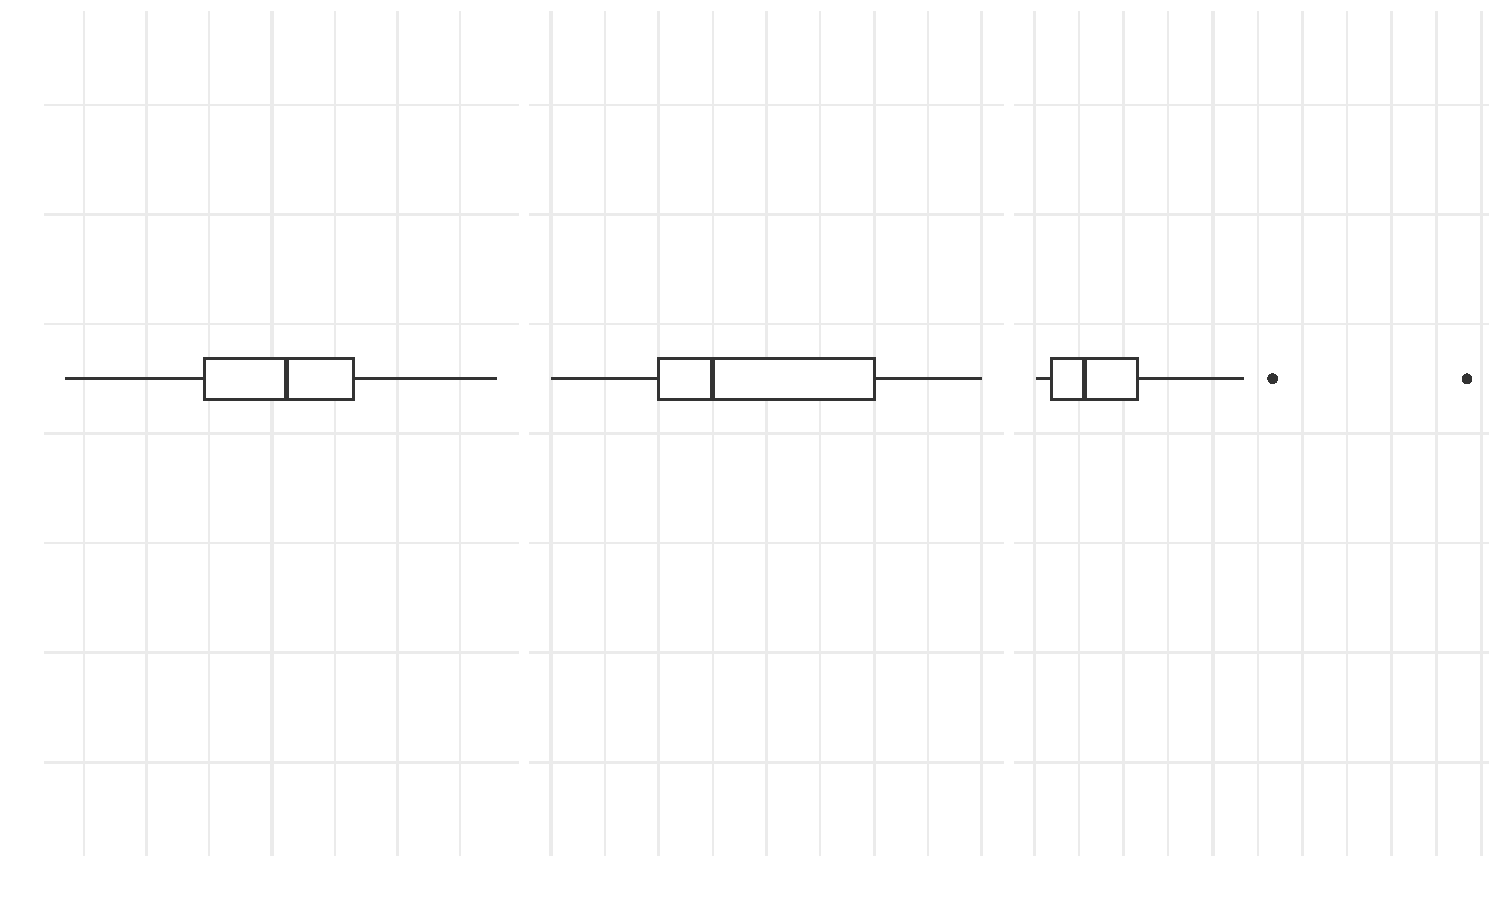
\includegraphics[width=\maxwidth]{img/desc-stat-11-1} 

}




Jetzt brauchen Tina und Alex Ihre Hilfe bei der Abschätzung einer Verteilung anhand von Boxplots um ihre Arbeit dann in diesem Semester noch abschließen zu können.

\begin{enumerate}
\item Zeichnen Sie über die Boxplots die entsprechende zugehörige Verteilung! \textbf{(3 Punkte)} 
\item Zeichnen Sie unter die Boxplots die entsprechende zugehörige Beobachtungen als Stiche! \textbf{(3 Punkte)}
\item Wie viel Prozent der Beobachtungen fallen in das IQR? Ergänzen Sie die Abbildung entsprechend um den Bereich! \textbf{(2 Punkte)}
\item Wie viel Prozent der Beobachtungen fallen in $\bar{y} \pm 1s$ und $\bar{y} \pm 2s$  unter der Annahme einer Normalverteilung? \textbf{(2 Punkte)}
\end{enumerate} 
\clearpage
% -----------------------------------------------------------------------

\section{Aufgabe \hfill (10 Punkte)}

\textit{Geben Sie grundsätzlich Formeln und Rechenweg zur Lösung der Teilaufgaben mit an!} \\[1Ex]
 

 
%% --------------------------------------------------------------------
\begin{minipage}[t]{0.5\textwidth}

\includegraphics[width = 1.3cm]{/Users/kruppajo/work/GitHub/exam/avatare/Jessica.png}\hspace{-4mm}
\includegraphics[width = 1.3cm]{/Users/kruppajo/work/GitHub/exam/avatare/Yuki.png}
\end{minipage}
\begin{minipage}[t]{0.5\textwidth}
\hfill
\href{https://youtu.be/ZrJhn2wPbq4}{
\includegraphics[width = 2cm]{img/youtube}}
\end{minipage}
%% --------------------------------------------------------------------



\paragraph{Visualisierung der Normalverteilung}

'Jetzt haben wir schon überall geschaut und ich finde die verdammte das Minischwein nicht. Wo ist die den normalerweise? Und wenn du jetzt einen blöden Witz über die Aufgabe und normal machst, dann gehe ich.', faucht Yuki Jessica an. 'Ui, alles gut. Vielleicht ein paar Schokobons zur Entspannung?', entgegnet Jessica. Manchmal macht die Faulheit Yuki zu einem anderen Menschen, der er nicht sein will. Da rennt dann auch das Minischwein vor ihm weg. Jetzt sollen die beiden diese Aufgabe zur Normalverteilung lösen. Es geht um verschiedene Normalverteilungen udn zu verstehen, wie die Parameter der Normalverteilung funktionieren. Anscheinend hängen Normalverteilungen vom Mittelwert $\bar{y}$ und der Standardabweichung $s$ ab.\\



Jetzt brauchen Yuki und Jessica Ihre Hilfe bei der Abschätzung einer Verteilung um ihre Arbeit dann in diesem Semester noch abschließen zu können.

\begin{enumerate}
\item Skizzieren Sie vier Normalverteilungen mit $\bar{y}_1 \neq \bar{y}_2 \neq \bar{y}_3 \neq \bar{y}_4$ und $s_1 \neq s_2 \neq s_3 \neq s_4$! \textbf{(3 Punkte)}
\item Beschriften Sie die Normalverteilungen mit den statistischen Maßzahlen! \textbf{(2 Punkte)}
\item Liegt Varianzhomogenität oder Varianzheterogenität vor? Begründen Sie Ihre Antwort! \textbf{(2 Punkte)}
\item In welchen Bereich fallen 68\% bzw. 95\% der Beobachtungen in einer Normalverteilung? Ergänzen Sie die Bereiche in \underline{einer} Normalverteilung! \textbf{(2 Punkte)}
\item Ergänzen Sie unter \underline{einer} der Normalverteilungen den entsprechenden Boxplot! \textbf{(1 Punkt)}
\end{enumerate}

 
\clearpage
% -----------------------------------------------------------------------

\section{Aufgabe \hfill (10 Punkte)}

\textit{Geben Sie grundsätzlich Formeln und Rechenweg zur Lösung der Teilaufgaben mit an!} \\[1Ex]
 

 
%% --------------------------------------------------------------------
\begin{minipage}[t]{0.5\textwidth}

\includegraphics[width = 1.3cm]{/Users/kruppajo/work/GitHub/exam/avatare/Mark.png}\hspace{-4mm}\includegraphics[width = 1.3cm]{/Users/kruppajo/work/GitHub/exam/avatare/Nilufar.png}
\end{minipage}
\begin{minipage}[t]{0.5\textwidth}
\hfill
\href{https://youtu.be/MiD42k4l5Ag}{\includegraphics[width = 2cm]{img/youtube}}
\end{minipage}
%% --------------------------------------------------------------------



\paragraph{Visualisierung der Normalverteilung und der Poissonverteilung}

'Was zum Geier?!', entfährt es Mark und schaut dabei Nilufar an. Dabei nimmt sogar der Hamster reißaus und versteckt sich unter dem Bett. 'Wir sollen eine Normalverteilung mit einem Mittelwert von $\bar{y}_1 = 0$ und einer Standardabweichung von $s_1 = 0.25$ zeichnen. Sowie eine weitere Normalverteilung mit einem Mittelwert von $\bar{y}_2 = 3$ und einer Standardabweichung von $s_2 = 0.25$. Keine Ahnung wie das geht. Darunter sollen dann noch eine Poissonverteilung mit einem Mittelwert von $\lambda_1 = 20$ sowie einer weiteren Poissonverteilung mit einem Mittelwert von $\lambda_2 = 3$ gezeichnet werden.', meint Nilufar sichtlich genervt und mampft noch ein paar Takis Blue Heat. Nilufar und die Erwartung machen die Suche nach der Lösung nicht einfacher. Im Hintergrund spielt viel zu leise Deichkind, die diesmal Nilufar ausgewählt hat.\\




{\centering \includegraphics[width=\maxwidth]{img/histogram-01-1} 

}




Jetzt brauchen Mark und Nilufar Ihre Hilfe bei der Abschätzung einer Verteilung um ihre Arbeit dann in diesem Semester noch abschließen zu können.


\begin{enumerate}
\item Skizzieren Sie die zwei Normalverteilungen und zwei Poissonverteilungen! \textbf{(4 Punkte)}
\item Achten Sie auf die entsprechende Skalierung in den jeweiligen Abbildungen! \textbf{(2 Punkte)}
\item Ergänzen Sie unter \underline{einer} Normalverteilung den entsprechenden Boxplot! \textbf{(1 Punkt)}
\item Ergänzen Sie unter \underline{einer} Poissonverteilung den entsprechenden Boxplot! \textbf{(1 Punkt)}
\item Geben Sie ein Beispiel für ein Outcome $y$, welches einer Normalverteilung folgt! \textbf{(1 Punkt)}
\item Geben Sie ein Beispiel für ein Outcome $y$, welches einer Poissonverteilung folgt! \textbf{(1 Punkt)}
\end{enumerate} 
\clearpage
% -----------------------------------------------------------------------
\part{Statistisches Testen \& statistische Testtheorie}
% -----------------------------------------------------------------------  

\section{Aufgabe \hfill (9 Punkte)}


 
%% --------------------------------------------------------------------
\begin{minipage}[t]{0.5\textwidth}
\includegraphics[width = 1.3cm]{/Users/kruppajo/work/GitHub/exam/avatare/Alex.png}\hspace{-4mm}\includegraphics[width = 1.3cm]{/Users/kruppajo/work/GitHub/exam/avatare/Nilufar.png}
\end{minipage}
\begin{minipage}[t]{0.5\textwidth}
\hfill
\href{https://youtu.be/aHVYuFKTqZs}{\includegraphics[width = 2cm]{img/youtube}}
\end{minipage}
%% --------------------------------------------------------------------



\paragraph{Grundgesamtheit und experimentelle Stichprobe}

'Grundlage des statistischen Testen ist das Verständnis von der Grundgesamtheit (eng. \textit{population} oder \textit{ground truth}) und der experimentellen Stichprobe (eng. \textit{sample}). ', liest Nilufar laut aus dem Skript vor. Alex war kurz eingenickt und wird mit einem Stoß geweckt. 'Reiz dich zusammen und iss noch ein paar Takis Blue Heat das hilft mir immer. Alleine komme ich hier nicht weiter.', tadelt Nilufar Alex etwas zu forsch. 'War ne lange Nacht', mault Alex. Beide sollen in ihrer Abschlussarbeit einen statistischen Test interpretieren und versuchen die Grundlagen zu wiederholen. Alex war auf einem Konzert von Abba.

\vspace{1ex}

Leider kennen sich Nilufar und Alex mit der Grundgesamtheit und der Stuchprobe überhaupt nicht aus. Daher sind Sie gefragt!

\begin{enumerate}
\item Nennen Sie das statistische Verfahren und zwei konkrete Beispiele zur Durchführung um von einer Grundgesamtheit auf eine Stichprobe zu gelangen! \textbf{(3 Punkte)}
\item Erklären Sie den Zusammenhang zwischen Stichprobe und Grundgesamtheit an einem Schaubild! Beschriften Sie das Schaubild entsprechend!
  \textit{Nutzen Sie hierfür als Veranschaulichung die Körpergröße von Männern oder Frauen aus den Gummibärchendaten!}  \textbf{(3 Punkte)}
\item Erweitern Sie das Schaubild um die Entstehung von $Pr(D|H_0)$! \textit{Nutzen Sie hierfür als Veranschaulichung zusätzlich die Gruppierungsvariable "`Modul"' aus den Gummibärchendaten!}  \textbf{(3 Punkte)}
\end{enumerate} 
\clearpage
% -----------------------------------------------------------------------

\section{Aufgabe \hfill (9 Punkte)}


 
%% --------------------------------------------------------------------
\begin{minipage}[t]{0.5\textwidth}
\includegraphics[width = 1.3cm]{/Users/kruppajo/work/GitHub/exam/avatare/Jonas.png}\hspace{-4mm}\includegraphics[width = 1.3cm]{/Users/kruppajo/work/GitHub/exam/avatare/Yuki.png}
\end{minipage}
\begin{minipage}[t]{0.5\textwidth}
\hfill
\href{https://youtu.be/Ric8ne39DtI}{\includegraphics[width = 2cm]{img/youtube}}
\end{minipage}
%% --------------------------------------------------------------------



\paragraph{Das Nullritual - Die statistische Testtheorie}

'Boldern ist der beste Sport, den es gibt.', meint Yuki. Jonas entgegnet, ' Ich empfehle ja immer allen Schwimmen.' Die beiden sind im Zoo und diskutieren, ob Pinguine Knie haben. Eigentlich wollten beide nochmal die statistische Testheorie durchgehen, sind dann aber auf abenteuerlichen Wege im Zoo gelandet. Yuki starrt wie hypnotisiert auf einen strullenden Elefanten und stopt die Zeit.\footnote{Yang, P. J., et al. (2014). Duration of urination does not change with body size. Proceedings of the National Academy of Sciences, 111(33), 11932-11937.} 'Du bist so peinlich.', entfährt es Jonas.

\vspace{1ex}

Leider kennen sich Yuki und Jonas mit statistischen Testtheorie, auch Null-Ritual genannt, überhaupt nicht aus. Geschweige denn mit der Visualisierung als Kreuztabelle.  

\begin{enumerate}
\item Tragen Sie folgende statistische Fachbegriffe zur statistischen Testtheorie korrekt eine selbst erstellte Kreuztabelle ein! \textbf{(3 Punkte)}
  \begin{center}
  \begin{tabular}{cccc}
  (Unbekannte) Wahrheit & Testentscheidung & H$_0$ wahr & H$_0$ beibehalten \\
  \end{tabular}
  \end{center}
\item Ergänzen Sie Ihre erstellte Kreuztabelle um vier weitere, passende Fachbegriffe zur statistischen Testtheorie! \textbf{(2 Punkte)}
\end{enumerate}

Die Entscheidungsfindung durch einen statistischen Test kann auch durch die Analogie zu einem Feuermelder abgebildet werden. Dabei symbolisiert der Feuermelder den statistischen Test und es soll getestet werden, ob ein Feuer ausgebrochen ist.

\begin{enumerate}
  \setcounter{enumi}{2}    
\item In der Analogie des Feuermelders, wie lautet der $\alpha$-Fehler? \textbf{(1 Punkt)}
\item In der Analogie des Feuermelders, wie lautet der $\beta$-Fehler? \textbf{(1 Punkt)}
\item Wenn der Feuermelder einmal pro Tag messen würde, wie oft würde der Feuermelder mit einem $\alpha$ von 5\% in einem Monat Alarm schlagen? Begründen Sie Ihre Antwort! \textbf{(2 Punkte)}
\end{enumerate}



 
\clearpage
% -----------------------------------------------------------------------

\section{Aufgabe \hfill (9 Punkte)}

\textit{Geben Sie grundsätzlich Formeln und Rechenweg zur Lösung der Teilaufgaben mit an!} \\[1Ex]


 
%% --------------------------------------------------------------------
\begin{minipage}[t]{0.5\textwidth}
\includegraphics[width = 1.3cm]{/Users/kruppajo/work/GitHub/exam/avatare/Mark.png}\hspace{-4mm}\includegraphics[width = 1.3cm]{/Users/kruppajo/work/GitHub/exam/avatare/Tina.png}
\end{minipage}
\begin{minipage}[t]{0.5\textwidth}
\hfill
\href{https://youtu.be/32JjH1eyuTU}{\includegraphics[width = 2cm]{img/youtube}}
\end{minipage}
%% --------------------------------------------------------------------



\paragraph{Visualisierung der Teststatistik $\boldsymbol{T_D}$ und dem p-Wert}

Tina und Mark wollten eigentlich einen Flug nach Mallorca buchen, sind jetzt aber dann doch dazu übergegangen nochmal die Aufgaben für die Statistikklausur durchzugehen. 'Kannst du mir nochmal an einer Visualisierung erklären, wie der Zusammenhang zwischen der Teststatistik aus den Daten $T_D$ und dem p-Wert ist? Ich habe hier zig Fachbegriffe, kriege die abr nicht zusammen...', fragt Tina. Mark zuckt mit den Schultern. So genau hatte Mark jetzt auch nicht aufgepasst. Da hilft dann eventuell das YouTube Video weiter. Tina mapmft Katjes und fragt sich, was das alles soll.

\vspace{1ex}

Leider kennen sich Tina und Mark mit der Visualisierung der Teststatistik $T_D$ und dem p-Wert überhaupt nicht aus und brauchen dahr Ihre Hilfe!

\vspace{1ex}

\textit{Beachten Sie, dass im Folgenden \underline{keine numerisch korrekte Darstellung} verlangt wird! Es gilt Erkennbarkeit vor Genauigkeit!}

\begin{enumerate}
\item Ergänzen Sie eine beschriftete $x$-Achse! \textbf{(1 Punkt)}
\item Ergänzen Sie "`$\bar{y}_1 = \bar{y}_2$"'! \textbf{(1 Punkt)} 
\item Ergänzen Sie "`$A = 95\%$"'! \textbf{(1 Punkt)}
\item Zeichnen Sie $T_{\alpha=5\%}$ in die Abbildung! \textbf{(1 Punkt)} 
\item Zeichnen Sie das Signifikanzniveau $\alpha$ in die Abbildung! Begründen Sie Ihre Antwort! \textbf{(2 Punkte)} 
\item Zeichnen Sie $-T_{D}$ in die Abbildung! \textbf{(1 Punkt)}
\item Zeichnen Sie einen signifikant p-Wert in die Abbildung! Begründen Sie Ihre Antwort! \textbf{(2 Punkte)}   
\end{enumerate}



{\centering \includegraphics[width=\maxwidth]{img/statistisches-testen-3-1} 

}


 
\clearpage
% -----------------------------------------------------------------------

\section{Aufgabe \hfill (10 Punkte)}


 
%% --------------------------------------------------------------------
\begin{minipage}[t]{0.5\textwidth}
\includegraphics[width = 1.3cm]{/Users/kruppajo/work/GitHub/exam/avatare/Alex.png}\hspace{-4mm}\includegraphics[width = 1.3cm]{/Users/kruppajo/work/GitHub/exam/avatare/Jessica.png}
\end{minipage}
\begin{minipage}[t]{0.5\textwidth}
\hfill
\href{https://youtu.be/CN_O4fYPbhs}{\includegraphics[width = 2cm]{img/youtube}}
\end{minipage}
%% --------------------------------------------------------------------



\paragraph{Visualisierung des 95\% Konfidenzintervalls}

'Okay, für was war jetzt nochmal das 95\% Konfidenzintervall gut?', fragt Jessica und schaut in das leere Gesicht von Alex. 'Keine Ahnung. Irgendwas mit Relevanz und Effekt oder Signifikanz. Da kannst du irgendwie was verbinden. Keine Ahnung warum', entgegnet Alex. 'Wir haben doch als Messwert \textit{Frischegewicht nach Bewässerung} erhoben.', stellt Jessica fest. Jetzt haben beide das Problem, die möglichen 95\% Konfidenzintervalle zu interpretieren.

\vspace{1ex}

Leider kennen sich Jessica und Alex mit der Visualisierung des 95\% Konfidenzintervall überhaupt nicht aus. 

\begin{enumerate}
\item Beschriften Sie die untenstehende Abbildung mit der Signifikanzschwelle! Begründen Sie Ihre Antwort! \textbf{(2 Punkte)}
\item Ergänzen Sie eine \textit{in den Kontext passende} Relevanzschwelle! Begründen Sie Ihre Antwort! \textbf{(2 Punkte)} 
\item Skizieren Sie in die untenstehende Abbildung sechs einzelne Konfidenzintervalle (a-f) mit den
  jeweiligen Eigenschaften! \textbf{(6 Punkte)}
  \begin{itemize}
  \item[(a)] Ein 95\% Konfidenzintervall mit h{"o}herer Varianz $s_p$ in der Stichprobe als der Rest der 95\% Konfidenzintervalle 	
  \item[(b)] Ein signifikantes, relevantes 90\% Konfidenzintervall. 	
  \item[(c)] Ein signifikantes, relevantes 95\% Konfidenzintervall 	
  \item[(d)] Ein nicht signifikantes, nicht relevantes 95\% Konfidenzintervall 
  \item[(e)] Ein signifikantes, nicht relevantes 95\% Konfidenzintervall
  \item[(f)] Ein 95\% Konfidenzintervall mit niedriger Varianz $s_p$ in der Stichprobe als der Rest 95\% der Konfidenzintervalle
  \end{itemize}
\end{enumerate}

\begin{center}
  \includegraphics[height = 10cm]{/Users/kruppajo/work/GitHub/exam/question/img/statistisches-testen-04}
\end{center}


 
\clearpage
% -----------------------------------------------------------------------

\section{Aufgabe \hfill (10 Punkte)}

\textit{Geben Sie grundsätzlich Formeln und Rechenweg zur Lösung der Teilaufgaben mit an!} \\[1Ex]


 
%% --------------------------------------------------------------------
\begin{minipage}[t]{0.5\textwidth}
\includegraphics[width = 1.3cm]{/Users/kruppajo/work/GitHub/exam/avatare/Alex.png}\hspace{-4mm}\includegraphics[width = 1.3cm]{/Users/kruppajo/work/GitHub/exam/avatare/Yuki.png}
\end{minipage}
\begin{minipage}[t]{0.5\textwidth}
\hfill
\href{https://youtu.be/FgZmpnEWDag}{\includegraphics[width = 2cm]{img/youtube}}
\end{minipage}
%% --------------------------------------------------------------------



\paragraph{Zusammenhang zwischen dem Effekt, der Streuung sowie der Fallzahl}

An einem kalten Dezembermorgen haben sich Alex und Yuki zum Lernen verabredet. Eine große Kanne Tee und Berge von Gummibärchen warten darauf gegessen zu werden. Alex liest laut vor:\begin{quote}
                 \textit{
                 Beim statistischen Testen gibt es einen Zusammenhang zwischen dem Effekt, der Streuung sowie der Fallzahl. Gegeben sei die Formel für den Student t-Test auf den die folgenden Überlegungen basieren sollen. Welche Auswirkung hat die Änderungen der jeweiligen statistischen Maßzahl des Effekts $\Delta$, der Streuung $s$ und der Fallzahl $n$ auf die Teststistik $T_{D}$, den p-Wert $Pr(D|H_0)$ sowie dem Konfidenzintervall $KI_{1-\alpha}$?
                 }
                 \end{quote}Yuki hebt die Augenbraue. 'Irgendwie sagt mir die Aufgabe jetzt mal so gar nichts. Was soll da gemacht werden?', merkt Yuki an und ergänzt: 'Schauen wir doch erstmal zur Entspannung Matrix, den Film habe ich extra nochmal mitgebracht.' Alex ist der Idee nicht abgeneigt und auch die Katze kommt unter dem Sofa hervor um mitzuschauen. 

\vspace{1ex}

Leider kennen sich Alex und Yuki mit dem Zusammenhang zwischen dem Effekt, der Streuung sowie der Fallzahl überhaupt nicht aus. 


\begin{enumerate}
\item Visualisieren Sie den Zusammenhang zwischen der Teststatiatik $T_{D}$ und dem p-Wert $Pr(D|H_0)$ für sich verändernde $T_{D}$-Werte!\textit{Geben Sie dafür ein numerisches Beispiel in dem Sie drei $T_{D}$-Werte und deren Einfluss auf den p-Wert vergleichen!} \textbf{(3 Punkte)}  
\item  Füllen Sie die untenstehende Tabelle aus in dem Sie die Änderung der statistischen Maßzahlen auf die Teststatistik, den p-Wert sowie das Konfidenzintervall in \textit{einem} Wort oder Symbol beschreiben! \textbf{(4 Punkte)}
\begin{center}
  \large
  \begin{tabular}[c]{l|c|c|c|l|c|c|c}
    & $T_{D}$ & $Pr(D|H_0)$ & $KI_{1-\alpha}$ & & $T_{D}$ & $Pr(D|H_0)$ & $KI_{1-\alpha}$\strut\\ 
    \hline
    \textbf{$\Delta\; \uparrow$} & \hspace{1.8cm} & \hspace{1.8cm}  & \hspace{1.8cm} & \textbf{
                                                          $\Delta\; \downarrow$} &
                                                                          \hspace{1.8cm} & \hspace{1.8cm}  & \hspace{1.8cm}\strut\\
    \hline
        \textbf{$s\; \uparrow$} & \hspace{1.8cm} & \hspace{1.8cm}  & \hspace{1.8cm} & \textbf{
                                                          $s\; \downarrow$} &
                                                                          \hspace{1.8cm}
                                                & \hspace{1.8cm}  & \hspace{1.8cm}\strut\\
    \hline
        \textbf{$n\; \uparrow$} & \hspace{1.8cm} & \hspace{1.8cm}  & \hspace{1.8cm} & \textbf{
                                                          $n\; \downarrow$} &
                                                                          \hspace{1.8cm}
                                                & \hspace{1.8cm}  & \hspace{1.8cm}\strut\\
    \hline
  \end{tabular}
\end{center}
\item Visualisieren Sie ein 95\%-iges Konfidenzintervall im Vergleich zu einem 99\%-igen Konfidenzintervall! Begründen Sie Ihre Visualisierung anhand der Formel des Konfidenzintervalls des t-Tests mathematisch! \textbf{(3 Punkte)} 
\end{enumerate} 
\clearpage
% -----------------------------------------------------------------------
\part{Der Student t-Test, Welch t-Test \& gepaarter t-Test}
% -----------------------------------------------------------------------

\section{Aufgabe \hfill (9 Punkte)}

\textit{Geben Sie grundsätzlich Formeln und Rechenweg zur Lösung der Teilaufgaben mit an!} \\[1Ex]
 

 
%% --------------------------------------------------------------------
\begin{minipage}[t]{0.5\textwidth}
\includegraphics[width = 1.3cm]{/Users/kruppajo/work/GitHub/exam/avatare/Steffen.png}
\end{minipage}
\begin{minipage}[t]{0.5\textwidth}
\hfill
\href{https://youtu.be/eejS2uG4o-M}{\includegraphics[width = 2cm]{img/youtube}}
\end{minipage}
\vspace{-3ex}
%% --------------------------------------------------------------------



\paragraph{Berechnung des Student t-Test \underline{oder} Welch t-Test}

'Der t-Test testet einen normalverteilten Endpunkt ($Y$).', liest Steffen laut. Das hilft jetzt auch nur bedingt weiter. Eine echte Herausforderung für ihn war schon immer die Romantik gewesen. Ein leidiges Lied. Laut seinem Betreuer ist zwar ihm Messwert Protein/Fettrate [\%/kg] normalverteilt, aber wie rechnet er jetzt einen t-Test? Für seine Abschlussarbeit zum Testen einer neuen technischen Anlage musste er ein Stallexperiment mit Milchvieh im Wendland durchführen. Als wäre das nicht schon anstrengend genug gewesen bei dem anspruchsvollen Pilotprojekt mit sehr geringer Fallzahl $(n_1 = n_2 = 3)$. Jetzt soll er auch noch testen, ob die Behandlung Ernährungszusatz ($ctrl$ und $fedX$) ein signifikantes Ergebnis liefert. Auf seinem Second Screen läuft Harry Potter und Steffen schaufelt Oreos. Nicht effizient, aber gut.

\begin{table}[!h]
\centering
\begin{tabular}{cc}
\toprule
treatment & weight\\
\midrule
dose & 27.9\\
dose & 17.8\\
ctrl & 20.9\\
ctrl & 23.9\\
dose & 25.3\\
\addlinespace
ctrl & 20.2\\
\bottomrule
\end{tabular}
\end{table}



Leider kennt sich Steffen mit der Berechnung eines t-Tests überhaupt nicht aus. Deshalb braucht er bei der Berechnung Ihre Hilfe!

\begin{enumerate}
  \item Formulieren Sie die wissenschaftliche Fragestellung! \textbf{(1 Punkt)}
  \item Bestimmen Sie die Teststatistik $T_{D}$ eines Welch t-Tests! \textbf{(3 Punkte)}
  \item Treffen Sie mit $T_{\alpha = 5\%} = 2.04$ eine Aussage zur Nullhypothese! Begründen Sie Ihre Antwort! \textbf{(2 Punkte)}
  \item Berechnen Sie den Effekt des Welch t-Tests! \textbf{(1 Punkt)}
  \item Formulieren Sie eine Antwort an Steffen über das Ergebnis Ihrer statistischen Analyse! \textbf{(2 Punkte)}
\end{enumerate} 
\clearpage
% -----------------------------------------------------------------------

\section{Aufgabe \hfill (12 Punkte)}

\textit{Geben Sie grundsätzlich Formeln und Rechenweg zur Lösung der Teilaufgaben mit an!} \\[1Ex]
 

 
%% --------------------------------------------------------------------
\begin{minipage}[t]{0.5\textwidth}
\includegraphics[width = 1.3cm]{/Users/kruppajo/work/GitHub/exam/avatare/Steffen.png}
\end{minipage}
\begin{minipage}[t]{0.5\textwidth}
\hfill
\href{https://youtu.be/Cq_rF_z4xOk}{\includegraphics[width = 2cm]{img/youtube}}
\end{minipage}
\vspace{-3ex}
%% --------------------------------------------------------------------



\paragraph{Berechnung des Student t-Test}

Die Uckermark, unendliche Weiten. Wir schreiben das Jahr 2024. Dies sind die Abenteuer von Steffen, der mit seiner 1 Mann starken Besatzung 12 Wochen lang unterwegs ist, um neue Welten zu erforschen, neues Leben und neue Zivilisationen. 'Oder nennen wir es Ödnis und Verzweiflung', denkt Steffen. Für seiner Hausarbeit ist Steffen ins Nichts gezogen. Eine echte Herausforderung für ihn war schon immer die Romantik gewesen. Ein leidiges Lied. Was macht er nun? Steffen hat einen Leistungssteigerungsversuch mit Zandern durchgeführt. Die Behandlung Flüssignahrung ($ctrl$ und $flOw$) wurde an Zandern getestet. Gemessen hat er dann als ein normalverteiltes Outcome ($Y$) Schlachtgewicht [kg]. Jetzt soll er seinem Betreuer nach testen, ob die Behandlung Flüssignahrung ($ctrl$ und $flOw$) ein signifikantes Ergebnis liefert. Hm..., was entspannendes wäre gut. Aus den Boxen wummert Taylor Swift und sein Mund ist verklebt von Oreos. 'Herrlich', denkt Steffen.

\begin{table}[!h]
\centering
\begin{tabular}{cc}
\toprule
Flüssignahrung & Schlachtgewicht\\
\midrule
flOw & 33.8\\
flOw & 33.6\\
ctrl & 33.5\\
flOw & 28.8\\
ctrl & 11.3\\
\addlinespace
ctrl & 9.8\\
flOw & 33.9\\
ctrl & 24.5\\
flOw & 33.7\\
ctrl & 29.1\\
\addlinespace
flOw & 39.5\\
ctrl & 36.3\\
flOw & 31.8\\
flOw & 40.1\\
ctrl & 17.8\\
\addlinespace
flOw & 33.7\\
ctrl & 25.6\\
\bottomrule
\end{tabular}
\end{table}



Leider kennt sich Steffen mit der Berechnung eines t-Tests überhaupt nicht aus. Deshalb braucht er bei der Berechnung Ihre Hilfe!

\begin{enumerate}
  \item Formulieren Sie die wissenschaftliche Fragestellung! \textbf{(1 Punkt)}
  \item Formulieren Sie das statistische Hypothesenpaar! \textbf{(1 Punkt)}
  \item Bestimmen Sie die Teststatistik $T_{D}$ eines Student t-Tests! \textbf{(3 Punkte)}
\item Treffen Sie mit $T_{\alpha = 5\%} = 1.96$ eine Aussage zur Nullhypothese! Begründen Sie Ihre Antwort! \textbf{(2 Punkte)}
\item Berechnen Sie den Effekt des Student t-Tests! \textbf{(1 Punkt)}
\item Wenn Sie \textit{keinen} Unterschied zwischen den Behandlungsgruppen erwarten würden, wie groß wäre dann die Teststatistik $T_{D}$? Begründen Sie Ihre Antwort! \textbf{(2 Punkte)}
\item Formulieren Sie eine Antwort an Steffen über das Ergebnis Ihrer statistischen Analyse! \textbf{(2 Punkte)}
\end{enumerate} 
\clearpage
% -----------------------------------------------------------------------

\section{Aufgabe \hfill (12 Punkte)}

\textit{Geben Sie grundsätzlich Formeln und Rechenweg zur Lösung der Teilaufgaben mit an!} \\[1Ex]
 

 
%% --------------------------------------------------------------------
\begin{minipage}[t]{0.5\textwidth}
\includegraphics[width = 1.3cm]{/Users/kruppajo/work/GitHub/exam/avatare/Mark.png}
\end{minipage}
\begin{minipage}[t]{0.5\textwidth}
\hfill
\href{https://youtu.be/TbSEOMCQYl4}{\includegraphics[width = 2cm]{img/youtube}}
\end{minipage}
\vspace{-3ex}
%% --------------------------------------------------------------------



\paragraph{Berechnung des Welch t-Test}


Mark ist im Teuteburgerwald für einen Versuch mit Brokkoli. Allein diese Tatsache ist für ihn eine Erzählung wert. Eine echte Herausforderung für ihn war schon immer die Unsicherheit gewesen. Ein leidiges Lied. Für seinen Projektbericht musste er einen Versuch in einer Klimakammer mit Brokkoli durchführen und das sollte laut seiner Betreuerin an diesem Nichtort besonders gut gelingen. Ablenkung gibt es jedenfalls keine. Gar keine. Alleine sein hilft jetzt aber nur bedingt, denn seine Behandlung Lichtstufen ($none$ und $600lm$) und der Messwert Proteingehalt [g/kg] sollen mit einem t-Test ausgewertet werden. Immerhin weiß er, dass sein Messwert einer Normalverteilung folgt. Hm..., was entspannendes wäre gut. Um zu Reiten geht Mark dann später nochmal raus. Echte Entspannung.

\begin{table}[!h]
\centering
\begin{tabular}{cc}
\toprule
Lichtstufen & Proteingehalt\\
\midrule
none & 39.5\\
600lm & 37.5\\
none & 28.3\\
none & 49.3\\
600lm & 27.1\\
\addlinespace
600lm & 19.1\\
none & 51.0\\
none & 33.0\\
600lm & 20.4\\
600lm & 22.7\\
\addlinespace
600lm & 17.1\\
none & 40.8\\
600lm & 29.0\\
600lm & 19.1\\
none & 28.0\\
\addlinespace
600lm & 21.4\\
600lm & 24.6\\
\bottomrule
\end{tabular}
\end{table}



Leider kennt sich Mark mit der Berechnung eines t-Tests überhaupt nicht aus. Deshalb braucht er bei der Berechnung Ihre Hilfe!

\begin{enumerate}
  \item Formulieren Sie die wissenschaftliche Fragestellung! \textbf{(1 Punkt)}
  \item Formulieren Sie das statistische Hypothesenpaar! \textbf{(1 Punkt)}
  \item Bestimmen Sie die Teststatistik $T_{D}$ eines  Welch t-Tests! \textbf{(3 Punkte)}
  \item Treffen Sie mit $T_{\alpha = 5\%} = 1.96$ eine Aussage zur Nullhypothese! Begründen Sie Ihre Antwort! \textbf{(2 Punkte)}
\item Berechnen Sie das 95\% Konfidenzintervall. Welche Annahmen haben Sie getroffen? \textbf{(2 Punkte)}
\item Nennen Sie den statistischen Grund, warum Sie sich zwischen einem Student t-Test und einem Welch t-Test entscheiden müssen! \textbf{(1 Punkt)}
\item Formulieren Sie eine Antwort an Mark über das Ergebnis Ihrer statistischen Analyse! \textbf{(2 Punkte)}
\end{enumerate} 
\clearpage
% -----------------------------------------------------------------------

\section{Aufgabe \hfill (11 Punkte)}

\textit{Geben Sie grundsätzlich Formeln und Rechenweg zur Lösung der Teilaufgaben mit an!} \\[1Ex]
 

 
%% --------------------------------------------------------------------
\begin{minipage}[t]{0.5\textwidth}
\includegraphics[width = 1.3cm]{/Users/kruppajo/work/GitHub/exam/avatare/Steffen.png}\hspace{-4mm}\includegraphics[width = 1.3cm]{/Users/kruppajo/work/GitHub/exam/avatare/Tina.png}
\end{minipage}
\begin{minipage}[t]{0.5\textwidth}
\hfill
\href{https://youtu.be/QR90zyn0Iz8}{\includegraphics[width = 2cm]{img/youtube}}
\end{minipage}
%% --------------------------------------------------------------------



\paragraph{Berechnung des gepaarten t-Test}

Steffen und Tina haben sich dazu entschieden zusammenzuarbeiten. Das sollte alles etwas einfacher machen. Jeder hat zwar ein getrenntes Themenfeld aber den Hauptversuch machen beide gemeinsam. Das hat sich schonmal als gut Idee soweit herausgestellt. In einem Projektbericht sollen beide herausfinden, ob es einen Zusammenhang zwischen Beschattung ($7d$ und $14d$) und Frischegewicht [kg/ha] gibt. Die Besonderheit ist hierbei, dass die Messungen an der gleichen Beobachtung stattfinden. Beide messen also zweimal an den gleichen Spargel. Hier muss dann wohl auf einen normalverteilten Messwert ($Y$) ein gepaarter t-Test gerechnet werden. Steffen schaut etwas flehentlich zu Tina. Eine echte Herausforderung für ihn war schon immer die Romantik gewesen. Ein leidiges Lied.. Steffen denkt derweil angestrengt an Tocotronic und wippt leicht mit dem Fuß.

\begin{table}[!h]
\centering
\begin{tabular}{ccc}
\toprule
ID & treatment & freshmatter\\
\midrule
3 & 7d & 35.8\\
7 & 7d & 21.6\\
8 & 14d & 6.3\\
10 & 14d & 22.1\\
6 & 14d & 44.9\\
\addlinespace
2 & 7d & 39.2\\
2 & 14d & 19.9\\
1 & 7d & 27.5\\
9 & 14d & 29.1\\
7 & 14d & 17.6\\
\addlinespace
4 & 14d & 33.6\\
11 & 14d & 27.0\\
5 & 7d & 29.2\\
4 & 7d & 24.2\\
5 & 14d & 24.8\\
\addlinespace
8 & 7d & 37.1\\
10 & 7d & 23.4\\
9 & 7d & 25.0\\
1 & 14d & 28.1\\
6 & 7d & 34.5\\
\addlinespace
3 & 14d & 17.3\\
\bottomrule
\end{tabular}
\end{table}



Leider kennen sich Steffen und Tina mit der Berechnung eines gepaarten t-Tests überhaupt nicht aus. Deshalb brauchen sie beide bei der Berechnung Ihre Hilfe!

\begin{enumerate}
  \item Formulieren Sie die wissenschaftliche Fragestellung! \textbf{(1 Punkt)}
  \item Formulieren Sie das statistische Hypothesenpaar! \textbf{(1 Punkt)}
  \item Bestimmen Sie die Teststatistik $T_{D}$ eines gepaarten t-Tests! \textbf{(3 Punkte)}
  \item Treffen Sie mit $T_{\alpha = 5\%} = 2.04$ eine Aussage zur Nullhypothese! Begründen Sie Ihre Antwort! \textbf{(2 Punkte)}
\item Schätzen Sie den $p$-Wert des gepaarten t-Tests ab! Begründen Sie Ihre Antwort mit einer Skizze! \textbf{(2 Punkte)}
\item Formulieren Sie eine Antwort an Steffen über das Ergebnis Ihrer statistischen Analyse! \textbf{(2 Punkte)}
\end{enumerate}


 
\clearpage
% -----------------------------------------------------------------------

\section{Aufgabe \hfill (10 Punkte)}

\textit{Geben Sie grundsätzlich Formeln und Rechenweg zur Lösung der Teilaufgaben mit an!} \\[1Ex]
 

 
%% --------------------------------------------------------------------
\begin{minipage}[t]{0.5\textwidth}
\includegraphics[width = 1.3cm]{/Users/kruppajo/work/GitHub/exam/avatare/Jonas.png}\hspace{-4mm}\includegraphics[width = 1.3cm]{/Users/kruppajo/work/GitHub/exam/avatare/Mark.png}\hspace{-4mm}\includegraphics[width = 1.3cm]{/Users/kruppajo/work/GitHub/exam/avatare/Tina.png}
\end{minipage}
\begin{minipage}[t]{0.5\textwidth}
\hfill
\href{https://youtu.be/exDo7AyHl4Q}{\includegraphics[width = 2cm]{img/youtube}}
\end{minipage}
%% --------------------------------------------------------------------



\paragraph{Interpretation des t-Tests in \Rlogo - die Teststatistik und der p-Wert}


'Wir waren in der Uckermark um Hühnern in einem Stallexperiment zu messen.', Mark legt das Dokument auf den Tisch und schaut Tina und Jonas fragend an. Beide schauen fragend zurück. Gäbe es die Erschöpfung nicht, dann wäre es für Jonas irgendwie einfacher hier zu helfen. Echt unangenehm. Die beiden sind zu Mark gekommen, da sie sich nicht mit \Rlogo auskennen und daher Hilfe bei der Interpretation des t-Tests brauchen. Im Hintergrund wummert Andrea Berg und leere Marzipankugeln Packungen stappeln sich auf dem Boden. 'Kein Problem', sagt Mark und streichelt langsam der Hamster. 'Aber worum es in dem Versuch geht, lässt sich nur aus dem Text in seiner Hand erahnen.' merkt er an. Vielleicht hilft da ja die Ausgabe des t-Tests in R weiter. Draußen geht blutrot die Sonne unter.

\begin{knitrout}
\definecolor{shadecolor}{rgb}{0.969, 0.969, 0.969}\color{fgcolor}\begin{kframe}
\begin{verbatim}
## 
## 	Two Sample t-test
## 
## data:  Protein/Fettrate by Elterlinie
## t = -7.338, df = 16, p-value = 1.669e-06
## alternative hypothesis: true  is not equal to [condensed]
## 95 percent confidence interval:
##  -23.69628 -13.07372
## sample estimates:
## mean in group Standard     mean in group Xray 
##                 25.440                 43.825
\end{verbatim}
\end{kframe}
\end{knitrout}

Helfen Sie Mark bei der Interpretation des t-Tests! Sonst geht es auch für Tina und Jonas nicht weiter.
  
\begin{enumerate}
  \item Formulieren Sie die wissenschaftliche Fragestellung! \textbf{(1 Punkt)}
  \item Formulieren Sie das statistische Hypothesenpaar! \textbf{(1 Punkt)}
\item Liegt ein signifikanter Unterschied zwischen den Gruppen vor? Begründen Sie Ihre Antwort! \textbf{(2 Punkte)}
\item Skizzieren Sie eine Abbildung in der Sie $T_{D}$, $Pr(D|H_0)$, $A=0.95$, sowie $T_{\alpha=5\%} = |2.12|$ einzeichnen! \textbf{(4 Punkte)}
\item Beschriften Sie die Abbildung! \textbf{(1 Punkt)}  
\item Berechnen Sie den Effekt des t-Tests! \textbf{(1 Punkt)}
\end{enumerate} 
\clearpage
% -----------------------------------------------------------------------

\section{Aufgabe \hfill (10 Punkte)}

\textit{Geben Sie grundsätzlich Formeln und Rechenweg zur Lösung der Teilaufgaben mit an!} \\[1Ex]
 

 
%% --------------------------------------------------------------------
\begin{minipage}[t]{0.5\textwidth}
\includegraphics[width = 1.3cm]{/Users/kruppajo/work/GitHub/exam/avatare/Mark.png}\hspace{-4mm}\includegraphics[width = 1.3cm]{/Users/kruppajo/work/GitHub/exam/avatare/Paula.png}\hspace{-4mm}\includegraphics[width = 1.3cm]{/Users/kruppajo/work/GitHub/exam/avatare/Tina.png}
\end{minipage}
\begin{minipage}[t]{0.5\textwidth}
\hfill
\href{https://youtu.be/wJqsNV1hOW8}{\includegraphics[width = 2cm]{img/youtube}}
\end{minipage}
%% --------------------------------------------------------------------



\paragraph{Interpretation des t-Tests in \Rlogo - das 95\% Konifidenzintervall}


'Wir waren im Emsland um Erdbeeren in einem Feldexperiment zu messen.', Tina legt das Dokument auf den Tisch und schaut Mark und Paula fragend an. Beide schauen fragend zurück. Gäbe es der Perfektionismus nicht, dann wäre es für Paula irgendwie einfacher hier zu helfen. Echt unangenehm. Die beiden sind zu Tina gekommen, da sie sich nicht mit \Rlogo auskennen und daher Hilfe bei der Interpretation des t-Tests brauchen. Im Hintergrund wummert Tocotronic und leere Katjes Packungen stappeln sich auf dem Boden. 'Kein Problem', sagt Tina und streichelt langsam die Spinne. 'Aber worum es in dem Versuch geht, lässt sich nur aus dem Text in seiner Hand erahnen.' merkt sie an. Vielleicht hilft da ja die Ausgabe des t-Tests in R weiter. Draußen geht blutrot die Sonne unter.

\begin{knitrout}
\definecolor{shadecolor}{rgb}{0.969, 0.969, 0.969}\color{fgcolor}\begin{kframe}
\begin{verbatim}
## 
## 	Two Sample t-test
## 
## data:  Proteingehalt by Genotypen
## t = -2.7068, df = 14, p-value = 0.01703
## alternative hypothesis: true  is not equal to [condensed]
## 95 percent confidence interval:
##  -13.4200  -1.5546
## sample estimates:
## mean in group AA mean in group BB 
##         21.95556         29.44286
\end{verbatim}
\end{kframe}
\end{knitrout}

Helfen Sie Tina bei der Interpretation des t-Tests! Sonst geht es auch für Mark und Paula nicht weiter.

\begin{enumerate}
  \item Formulieren Sie die wissenschaftliche Fragestellung! \textbf{(1 Punkt)}
  \item Formulieren Sie das statistische Hypothesenpaar! \textbf{(1 Punkt)}
\item Liegt ein signifikanter Unterschied zwischen den Gruppen vor? Begründen Sie Ihre Antwort! \textbf{(2 Punkte)}
\item Skizieren Sie das sich ergebende 95\% Konifidenzintervall! \textbf{(2 Punkte)}
\item Beschriften Sie die Abbildung und das 95\% Konfidenzintervall entsprechend! \textbf{(2 Punkte)}  
\item Interpretieren Sie den Effekt des 95\% Konifidenzintervalls! \textbf{(2 Punkte)}
\end{enumerate} 
\clearpage
% -----------------------------------------------------------------------

\section{Aufgabe \hfill (9 Punkte)}

\textit{Geben Sie grundsätzlich Formeln und Rechenweg zur Lösung der Teilaufgaben mit an!} \\[1Ex]
 

 
%% --------------------------------------------------------------------
\begin{minipage}[t]{0.5\textwidth}
\includegraphics[width = 1.3cm]{/Users/kruppajo/work/GitHub/exam/avatare/Alex.png}\hspace{-4mm}\includegraphics[width = 1.3cm]{/Users/kruppajo/work/GitHub/exam/avatare/Mark.png}\hspace{-4mm}\includegraphics[width = 1.3cm]{/Users/kruppajo/work/GitHub/exam/avatare/Steffen.png}
\end{minipage}
\begin{minipage}[t]{0.5\textwidth}
\hfill
\href{https://youtu.be/w62HJlbN28U}{\includegraphics[width = 2cm]{img/youtube}}
\end{minipage}
%% --------------------------------------------------------------------



\paragraph{Interpretation des t-Tests in \Rlogo - die Visualisierung}

'Wir sind uns relativ sicher, dass unser Messwert Schlachtgewicht [kg] ist!', ruft Mark wild gestikulierend. Mark wäre mehr präsent, wenn es die Unsicherheit nicht gäbe. Als würde sowas die Ausgabe von \Rlogo interessieren. Mark und Alex sind in einem Cafè mit Steffen um sich Hilfe von ihm in \Rlogo zu holen. Während Steffen Kirschstreuselkuchen und Oreos mampft, versuchen die Mark und Alex ihren Versuch in der Uckermark mit Zandern in einem Leistungssteigerungsversuch zu erklären. Steffen hofft insgeheim, dass die \Rlogo Ausgabe des t-Tests ihm mehr Informationen liefert. Eigentlich würde er dann doch lieber raus um zu Ringen vielleicht mit Alex?

\begin{knitrout}
\definecolor{shadecolor}{rgb}{0.969, 0.969, 0.969}\color{fgcolor}\begin{kframe}
\begin{verbatim}
## 
## 	Two Sample t-test
## 
## data:  Schlachtgewicht by Lüftungssystem
## t = 0.24886, df = 13, p-value = 0.8074
## alternative hypothesis: true  is not equal to [condensed]
## 95 percent confidence interval:
##  -8.407997 10.597283
## sample estimates:
##     mean in group keins mean in group vorhanden 
##                25.55714                24.46250
\end{verbatim}
\end{kframe}
\end{knitrout}

Helfen Sie Steffen bei der Interpretation des t-Tests! Sonst geht es auch für Mark und Alex nicht weiter.
  
\begin{enumerate}
  \item Formulieren Sie die wissenschaftliche Fragestellung! \textbf{(1 Punkt)}
  \item Formulieren Sie das statistische Hypothesenpaar! \textbf{(1 Punkt)}
\item Liegt ein signifikanter Unterschied zwischen den Gruppen vor? Begründen Sie Ihre Antwort! \textbf{(2 Punkte)}
\item Skizieren Sie die sich ergebenden Boxplot! Welche Annahmen an die Daten haben Sie getroffen? Begründen Sie Ihre
  Antwort! \textbf{(2 Punkte)} 
\item Skizieren Sie die sich ergebenden Barplots! \textbf{(2 Punkte)}
\item Berechnen Sie den Effekt des t-Tests! \textbf{(1 Punkt)}
\end{enumerate}
 
\clearpage
% -----------------------------------------------------------------------

\section{Aufgabe \hfill (10 Punkte)}

\textit{Geben Sie grundsätzlich Formeln und Rechenweg zur Lösung der Teilaufgaben mit an!} \\[1Ex]
 

 
%% --------------------------------------------------------------------
\begin{minipage}[t]{0.5\textwidth}
\includegraphics[width = 1.3cm]{/Users/kruppajo/work/GitHub/exam/avatare/Paula.png}\hspace{-4mm}\includegraphics[width = 1.3cm]{/Users/kruppajo/work/GitHub/exam/avatare/Steffen.png}
\end{minipage}
\begin{minipage}[t]{0.5\textwidth}
\hfill
\href{https://youtu.be/kHmfEmU6lrk}{\includegraphics[width = 2cm]{img/youtube}}
\end{minipage}
%% --------------------------------------------------------------------



\paragraph{Interpretation des gepaarten t-Tests in \Rlogo}

Alles voll mit Puten. Aber das haben Paula und Steffen eben gemeinsam in einer Hausarbeit gemacht! Worum ging es aber konkret? Beide haben als einen normalverteilten Endpunkt ($Y$) Gewichtszuwachs in der 1LW von Puten bestimmt. Die Daten haben beide zusammen in einem Kreuzungsexperiment erhoben. In dem Experiment ging es um eine vorher/nachher Untersuchung an den gleichen Puten. Als Behandlung wurde Ernährungszusatz ($ohne$ und $14d$) eingesetzt. Nach der Meinung des Betreuers muss hier ein gepaarter t-Test gerechnet werden. Leider kennen sich beide nicht sehr gut in \Rlogo aus. Paula hat einiges an Smarties geholt, so dass beide die Zeit gut durchbringen werden. Dann geht Paula nochmal zum Sport. Paula will später nochmal raus um zu Fechten. Druck ablassen, dass muss sie auch.

\begin{knitrout}
\definecolor{shadecolor}{rgb}{0.969, 0.969, 0.969}\color{fgcolor}\begin{kframe}
\begin{verbatim}
## 
## 	Paired t-test
## 
## data:  Gewichtszuwachs by Ernährungszusatz
## t = -0.76287, df = 8, p-value = 0.4674
## alternative hypothesis: true  is not equal to [condensed]
## 95 percent confidence interval:
##  -9.565315  4.809759
## sample estimates:
## mean difference 
##       -2.377778
\end{verbatim}
\end{kframe}
\end{knitrout}

Jetzt brauchen Paula und Steffen Ihre Hilfe bei der Berechnung eines gepaarten t-Tests in \Rlogo um ihre Arbeit dann in diesem Semester noch abschließen zu können.

\begin{enumerate}
  \item Formulieren Sie die wissenschaftliche Fragestellung! \textbf{(1 Punkt)}
  \item Formulieren Sie das statistische Hypothesenpaar! \textbf{(1 Punkt)}
\item Liegt ein signifikanter Unterschied zwischen den Gruppen vor?
  Begründen Sie Ihre Antwort! \textbf{(2 Punkte)}
\item Skizzieren Sie das sich ergebende 95\% Konfidenzintervall! \textbf{(2 Punkte)}
\item Interpretieren Sie den Effekt des gepaarten t-Tests! \textbf{(2 Punkte)}
\item Skizzieren Sie den sich ergebenden Boxplot der Differenzen! Welche Annahmen an die Daten haben Sie getroffen? Begründen Sie Ihre Antwort! \textbf{(2 Punkte)} 
\end{enumerate}
 
\clearpage
% -----------------------------------------------------------------------
\part{Die einfaktorielle \& zweifaktorielle ANOVA}
% -----------------------------------------------------------------------

\section{Aufgabe \hfill (11 Punkte)}

\textit{Geben Sie grundsätzlich Formeln und Rechenweg zur Lösung der Teilaufgaben mit an!} \\[1Ex]
 

 
%% --------------------------------------------------------------------
\begin{minipage}[t]{0.5\textwidth}
\includegraphics[width = 1.3cm]{/Users/kruppajo/work/GitHub/exam/avatare/Nilufar.png}\hspace{-4mm}\includegraphics[width = 1.3cm]{/Users/kruppajo/work/GitHub/exam/avatare/Paula.png}
\end{minipage}
\begin{minipage}[t]{0.5\textwidth}
\hfill
\href{https://youtu.be/kHmfEmU6lrk}{\includegraphics[width = 2cm]{img/youtube}}
\end{minipage}
%% --------------------------------------------------------------------



\paragraph{Visualisierung der einfaktoriellen ANOVA}

'Uff... die einfaktorielle ANOVA. Und wir können jetzt anhand der Visualisuierung sehen, ob da schon was signifikant ist?', Paula hebt die Augenbraue. 'Ja, können wir. Dafür müssen wir aber erstmal in \texttt{\{ggplot\}} uns die Daten anschauen. Oder wir zeichnen es flott mit der Hand. Geht auch.', meint Nilufar dazu. Die beiden hatten sich auf einem Konzert von Deichkind kennengelernt. Paula hatte sich in ein Kreuzungsexperiment verschiedene Puten angeschaut. Dabei ging es herauszufinden, ob es einen Zusammenhang zwischen der Behandlung Ernährungszusatz ($ctrl$, $fedX$ und $getIt$) und dem Messwert Schlachtgewicht [kg] gibt. Später wird noch Star Trek geguckt. Nilufar befürwortet das!

\begin{knitrout}
\definecolor{shadecolor}{rgb}{0.969, 0.969, 0.969}\color{fgcolor}\begin{table}[!h]
\centering
\begin{tabular}{cc}
\toprule
Ernährungszusatz & Schlachtgewicht\\
\midrule
getIt & 30\\
ctrl & 29\\
getIt & 30\\
fedX & 44\\
ctrl & 32\\
\addlinespace
fedX & 45\\
fedX & 43\\
ctrl & 27\\
fedX & 44\\
getIt & 30\\
\addlinespace
ctrl & 31\\
fedX & 44\\
ctrl & 33\\
fedX & 44\\
fedX & 44\\
\addlinespace
getIt & 30\\
getIt & 31\\
getIt & 30\\
getIt & 30\\
\bottomrule
\end{tabular}
\end{table}

\end{knitrout}

Leider kennen sich Paula und Nilufar mit Darstellung einer einfaktoriellen ANOVA überhaupt nicht aus. 

\begin{enumerate}
\item Erstellen  Sie  eine  Visualisierung  der  Datentabelle! Beschriften  Sie  die  Abbildung! \textbf{(2 Punkte)}
\item Benennen Sie die Visualisierung mit dem korrekten, statistischen Fachbegriff! \textbf{(1 Punkt)}
\item Zeichnen Sie folgende statistischen Maßzahlen passend ein! 
  \begin{itemize}
  \item Globale Mittelwert: $\beta_0$ \textbf{(1 Punkt)}
  \item Mittelwerte der einzelnen Behandlungsstufen: $\bar{y}_{0.5}$, $\bar{y}_{1.5}$ und $\bar{y}_{2.5}$ \textbf{(1 Punkt)}
  \item Mittelwertsdifferenz der einzelnen Behandlungsstufen: $\beta_{0.5}$, $\beta_{1.5}$ und $\beta_{2.5}$ \textbf{(1 Punkt)}
  \item Residuen oder Fehler: $\epsilon$ \textbf{(1 Punkt)}
  \end{itemize}
\item Liegt ein \textit{vermutlicher} signifikanter Unterschied vor? Begründen Sie Ihre Antwort! \textbf{(2 Punkte)}
\item Schätzen Sie die Effekte der Behandlungsstufen! \textbf{(2 Punkte)}
\end{enumerate}
 
\clearpage
% -----------------------------------------------------------------------

\section{Aufgabe \hfill (9 Punkte)}

\textit{Geben Sie grundsätzlich Formeln und Rechenweg zur Lösung der Teilaufgaben mit an!} \\[1Ex]
 

 
%% --------------------------------------------------------------------
\begin{minipage}[t]{0.5\textwidth}
\includegraphics[width = 1.3cm]{/Users/kruppajo/work/GitHub/exam/avatare/Mark.png}\hspace{-4mm}\includegraphics[width = 1.3cm]{/Users/kruppajo/work/GitHub/exam/avatare/Nilufar.png}
\end{minipage}
\begin{minipage}[t]{0.5\textwidth}
\hfill
\href{https://youtu.be/IhecxMcCENY}{\includegraphics[width = 2cm]{img/youtube}}
\end{minipage}
%% --------------------------------------------------------------------



\paragraph{Ergebnistabelle der einfaktoriellen ANOVA}

'Als erstes bauen wir uns aus unsere Daten die ANOVA Tabelle dann sehen wir schon, ob unser Gruppenvergleich in der ANOVA signifikant ist.', Mark schaut Nilufar fragend an und hofft auf eine positive Regung im Gesicht. Wird aber enttäuscht. Da hilft das Huhn von Nilufar auch nur bedingt. Nilufar tut sich auch sehr schwer mit der einfaktoriellen ANOVA. Beide waren in der Uckermark um ein Kreuzungsexperiment mit Hühnern durchzuführen. Dabei ging es herauszufinden, ob es einen Zusammenhang zwischen der Behandlung Flüssignahrung ($ctrl$, $superIn$ und $flOw$) und dem Messwert Fettgehalt [\%/kg] gibt. Nachher wollen sich beide noch mit dem Hobby Hip Hop von Nilufar beschäftigen. Kennt Mark noch nicht, klingt aber interessant.



\vspace{1ex}

Leider kennen sich Mark und Nilufar mit Berechnung einer einfaktoriellen ANOVA überhaupt nicht aus. Deshalb brauchen beide bei der Erstellung Ihre Hilfe, das Huhn reicht als Hilfe nicht aus! 

\begin{enumerate}
  \item Formulieren Sie die wissenschaftliche Fragestellung! \textbf{(1 Punkt)}
  \item Formulieren Sie das statistische Hypothesenpaar! \textbf{(1 Punkt)}
\item Füllen Sie die unterstehende einfaktorielle ANOVA Ergebnistabelle aus! \textbf{(3 Punkte)}
\end{enumerate}

\vspace{1Ex}

\begin{center}
  \Large
  \begin{tabular}{lccccp{3cm}}
\toprule
     & \textbf{Df} & \textbf{Sum Sq} & \textbf{Mean Sq} & \textbf{F value} & \textbf{Pr(>F)} \strut\\
    \midrule
   \textbf{Flüssignahrung}  & 2 &  &  &  &  \strut\\
   \textbf{error}  & 14 & 872.17 &  &  &  \strut\\
   \textbf{Total}  & 16 & 2090.94 &  &  &  \strut\\
\bottomrule
  \end{tabular}
\end{center}

\vspace{1Ex}

\begin{enumerate}
  \setcounter{enumi}{3}
\item Schätzen Sie den p-Wert der Tabelle mit $F_{\alpha = 5\%} = 3.74$ ab. Begründen Sie Ihre Antwort! \textbf{(2 Punkte)}
\item Berechen Sie den Effektschätzer $\eta^2$. Was sagt Ihnen der Wert von $\eta^2$ aus? \textbf{(2 Punkte)}
\end{enumerate}



 
\clearpage
% -----------------------------------------------------------------------

\section{Aufgabe \hfill (12 Punkte)}

\textit{Geben Sie grundsätzlich Formeln und Rechenweg zur Lösung der Teilaufgaben mit an!} \\[1Ex]
 

 
%% --------------------------------------------------------------------
\begin{minipage}[t]{0.5\textwidth}
\includegraphics[width = 1.3cm]{/Users/kruppajo/work/GitHub/exam/avatare/Jessica.png}\hspace{-4mm}\includegraphics[width = 1.3cm]{/Users/kruppajo/work/GitHub/exam/avatare/Yuki.png}
\end{minipage}
\begin{minipage}[t]{0.5\textwidth}
\hfill
\href{https://youtu.be/49hvImMwVyE}{\includegraphics[width = 2cm]{img/youtube}}
\end{minipage}
%% --------------------------------------------------------------------



\paragraph{Die einfaktoriellen ANOVA und der Student t-Test}

Yuki und Jessica schauen sich etwas entnervt an. Gemeinsam schreiben die beiden ihre Abschlussarbeit und sollen nun als erstes einmal die Daten mit eine einfaktoriellen ANOVA auswerten damit abgeschätzt werden kann, ob überhaupt signifikante Ergebnisse in den multipen Gruppenvergleichen zu erwarten sind. Deshalb erstmal Schokobons mampfen, die Jessica mitgebracht hat. Nun möchte erstmal ihre Betreuung der Arbeit eine ANOVA Tabelle sehen. Was immer da auch drin zu erkennen sein mag. Yuki schaut Jessica sehen erstmla gar nichts. Die beiden waren in der Uckermark um ein Freilandversuch mit Erdbeeren durchzuführen. Dabei haben Yuki und Jessica den Messwert Proteingehalt [g/kg] unter der Behandung Substrattypen ($torf$, $40p60n$, $30p20n$ und $70p30n$) ermittelt. Später wollen die beiden dann noch raus um Rad zu fahren.



\vspace{1ex}

Leider kennen sich Yuki und Jessica mit Berechnung einer einfaktoriellen ANOVA überhaupt nicht aus. Deshalb brauchen beide bei der Erstellung Ihre Hilfe! 

\begin{enumerate}
  \item Formulieren Sie die wissenschaftliche Fragestellung! \textbf{(1 Punkt)}
  \item Formulieren Sie das statistische Hypothesenpaar! \textbf{(1 Punkt)}
\item Füllen Sie die unterstehende einfaktorielle ANOVA Ergebnistabelle aus! \textbf{(3 Punkte)}
\end{enumerate}

\vspace{1Ex}

\begin{center}
  \Large
  \begin{tabular}{lccccp{3cm}}
\toprule
     & \textbf{Df} & \textbf{Sum Sq} & \textbf{Mean Sq} & \textbf{F value} & \textbf{Pr(>F)} \strut\\
    \midrule
   \textbf{Substrattypen}  & 3 & 445.26 &  &  &  \strut\\
   \textbf{Error}  & 25 & 549.56 &  &  &  \strut\\
\bottomrule
  \end{tabular}
\end{center}

\vspace{1Ex}

\begin{enumerate}
  \setcounter{enumi}{3}
\item Schätzen Sie den p-Wert der Tabelle mit $F_{\alpha = 5\%} = 2.99$ ab. Begründen Sie Ihre Antwort! \textbf{(2 Punkte)}
\item Was bedeutet ein signifikantes Ergebnis in einer einfaktoriellen ANOVA? \textbf{(1 Punkt)}
\item Berechnen Sie \textit{einen} Student t-Test für den \textit{vermutlich} signifikantesten Gruppenvergleich anhand der untenstehenden Tabelle mit $T_{\alpha = 5\%} = 2.03$. Begründen Sie Ihre Auswahl! \textbf{(3 Punkte)}
\end{enumerate}


\begin{knitrout}
\definecolor{shadecolor}{rgb}{0.969, 0.969, 0.969}\color{fgcolor}\begin{table}[!h]
\centering\begingroup\fontsize{11}{13}\selectfont

\begin{tabular}{cccc}
\toprule
\textbf{Substrattypen} & \textbf{Fallzahl (n)} & \textbf{Mittelwert} & \textbf{Standardabweichung}\\
\midrule
torf & 8 & 14.62 & 7.39\\
40p60n & 7 & 7.00 & 2.65\\
30p20n & 5 & 4.80 & 2.59\\
70p30n & 9 & 5.89 & 3.52\\
\bottomrule
\end{tabular}
\endgroup{}
\end{table}

\end{knitrout}


\begin{enumerate}
  \setcounter{enumi}{6}
\item Gegebenen der ANOVA Tabelle war das Ergebnis des Student t-Tests zu erwarten? Begründen Sie Ihre Antwort! \textbf{(2 Punkte)}
\end{enumerate}

 
\clearpage
% -----------------------------------------------------------------------

\section{Aufgabe \hfill (9 Punkte)}

\textit{Geben Sie grundsätzlich Formeln und Rechenweg zur Lösung der Teilaufgaben mit an!} \\[1Ex]
 

 
%% --------------------------------------------------------------------
\begin{minipage}[t]{0.5\textwidth}
\includegraphics[width = 1.3cm]{/Users/kruppajo/work/GitHub/exam/avatare/Jessica.png}
\end{minipage}
\begin{minipage}[t]{0.5\textwidth}
\hfill
\href{https://youtu.be/aXvxGC4YLqk}{\includegraphics[width = 2cm]{img/youtube}}
\end{minipage}
\vspace{-3Ex}
%% --------------------------------------------------------------------



\paragraph{Die einfaktorielle ANOVA in \Rlogo}

'Uff... die einfaktorielle ANOVA und \Rlogo. Nicht so einfach... Was sagt mir jetzt die Ausgabe der ANOVA und wo sehe ich, ob da was signifikant ist?', denkt Jessica und hebt die Augenbraue. Jessica hatte sich ein Kreuzungsexperiment mit Lamas angeschaut. Als wäre das nicht alles schon schwer genug. Jessica und der Mangel, eine unendliche Geschichte mit kniffeligen Wendungen. Dabei ging es beim Experiment herauszufinden, ob es einen Zusammenhang zwischen der Behandlung Flüssignahrung ($ctrl$, $superIn$ und $flOw$) und dem Messwert Schlachtgewicht [kg] gibt. Nun möchte ihre Betreuerin ihrer Abschlussarbeit erstmal eine ANOVA sehen und die Ergebnisse präsentiert bekommen. Und eigentlich will sie ja was anderes... Hm, lecker Schokobons und dazu dann im Hintergrund Herr der Ringe laufen lassen.

\begin{knitrout}
\definecolor{shadecolor}{rgb}{0.969, 0.969, 0.969}\color{fgcolor}\begin{kframe}
\begin{verbatim}
## Analysis of Variance Table
## 
## Response: Schlachtgewicht
##                Df Sum Sq Mean Sq F value Pr(>F)
## Flüssignahrung  2  94.57  47.283  2.1415 0.1465
## Residuals      18 397.43  22.080
\end{verbatim}
\end{kframe}
\end{knitrout}

\vspace{1ex}

Leider kennen sich Jessica mit Berechnung einer einfaktoriellen ANOVA überhaupt nicht aus. Deshalb braucht sie bei der Erstellung Ihre Hilfe! 

\begin{enumerate}
  \item Formulieren Sie die wissenschaftliche Fragestellung! \textbf{(1 Punkt)}
  \item Formulieren Sie das statistische Hypothesenpaar! \textbf{(1 Punkt)}
\item Interpretieren Sie das Ergebnis der einfaktoriellen ANOVA! \textbf{(2 Punkte)} 
\item Berechnen Sie den Effektschätzer $\eta^2$. Was sagt Ihnen der Wert von $\eta^2$ aus? \textbf{(2 Punkte)}
\item Skizzieren Sie eine Abbildung, der dem obigen Ergebnis der
  einfaktoriellen ANOVA näherungsweise entspricht! \textbf{(3 Punkte)}
\end{enumerate}

 
\clearpage
% -----------------------------------------------------------------------

\section{Aufgabe \hfill (12 Punkte)}

\textit{Geben Sie grundsätzlich Formeln und Rechenweg zur Lösung der Teilaufgaben mit an!} \\[1Ex]
 

 
%% --------------------------------------------------------------------
\begin{minipage}[t]{0.5\textwidth}
\includegraphics[width = 1.3cm]{/Users/kruppajo/work/GitHub/exam/avatare/Paula.png}
\end{minipage}
\begin{minipage}[t]{0.5\textwidth}
\hfill
\href{https://youtu.be/8Pb2sKUIMyk}{\includegraphics[width = 2cm]{img/youtube}}
\end{minipage}
\vspace{-3Ex}
%% --------------------------------------------------------------------



\paragraph{Ergebnistabelle der zweifaktoriellen ANOVA}

In einen Versuch in einer Klimakammer wurden Erbsen mit dem Behandlung Düngestufen ($ctrl$, $low$, $mid$ und $high$) sowie der Behandlung Substrattypen ($torf$, $70p30n$) untersucht. Es wurde als Messwert Proteingehalt [g/kg] bestimmt. Paula ahnte schon, dass es komplexer wird, als sie mit ihrem Projektbericht angefangen hat. Das es jetzt aber so kompliziert wird, hätte sie jetzt aber auch nicht gedacht. Paula kratzt sich am Kopf. Paula mampft aus Frust noch eine Handvoll Smarties. Eventuell muss sie dann doch nochmal Hilfe in der statistischen Beratung holen. Jetzt versucht sie es aber erstmal selber. Und eigentlich wollte Paula doch noch ihrem Hobby nachgehen! Harry Potter. Ein wunderbares Hobby um sich drin zu verlieren und Abstand zu bekommen. Paula denkt gerne über Harry Potter nach.



\vspace{1ex}

Leider kennen sich Paula mit Berechnung einer zweifaktoriellen ANOVA überhaupt nicht aus. Deshalb braucht sie bei der Erstellung Ihre Hilfe! 

\begin{enumerate}
  \item Formulieren Sie die wissenschaftliche Fragestellung! \textbf{(1 Punkt)}
  \item Formulieren Sie das statistische Hypothesenpaar! \textbf{(1 Punkt)}
\item Füllen Sie die unterstehende einfaktorielle ANOVA Ergebnistabelle aus! \textbf{(3 Punkte)}
\end{enumerate}

\vspace{1Ex}

\begin{center}
  \Large
  \begin{tabular}{lccccc}
  \toprule
     & \textbf{Df} & \textbf{Sum Sq} & \textbf{Mean Sq} & \textbf{F value} & \textbf{Pr(>F)} \strut\\
    \midrule
   \textbf{Düngestufen}  & 3 & 3.04 &  &  &  \strut\\
    \textbf{Substrattypen}  & 1 & 220.16 &  &  &  \strut\\
    \textbf{Düngestufen:Substrattypen}  & 3 & 127.38 &  &  &  \strut\\
   \textbf{Error}  & 18 & 290.92 &  &  &  \strut\\
\bottomrule
  \end{tabular}
\end{center}

\vspace{1Ex}

\begin{enumerate}
  \setcounter{enumi}{3}
\item Schätzen Sie den p-Wert der Tabelle ab. Begründen Sie Ihre
  Antwort! \textbf{(3 Punkte)}
\end{enumerate}
  
\begin{center}
    \Large
\begin{tabular}{lc}
  \toprule
     & $\boldsymbol{F_{\alpha = 5\%}}$ \\
\midrule
  \textbf{Düngestufen} & $4.26$ \\
  \textbf{Substrattypen} & $3.40$ \\
  \textbf{Düngestufen:Substrattypen} & $5.23$ \\
  \bottomrule
  \end{tabular}
\end{center}

\begin{enumerate}
  \setcounter{enumi}{4}
\item Was bedeutet ein signifikantes Ergebnis in einer zweifaktoriellen ANOVA? \textbf{(2 Punkte)}
\item Was sagt der Term \textit{Düngestufen:Substrattypen} aus? Interpretieren Sie das Ergebnis! \textbf{(2 Punkte)}
\end{enumerate}
 
\clearpage
% -----------------------------------------------------------------------

\section{Aufgabe \hfill (10 Punkte)}

\textit{Geben Sie grundsätzlich Formeln und Rechenweg zur Lösung der Teilaufgaben mit an!} \\[1Ex]
 

 
%% --------------------------------------------------------------------
\begin{minipage}[t]{0.5\textwidth}
\includegraphics[width = 1.3cm]{/Users/kruppajo/work/GitHub/exam/avatare/Jessica.png}
\end{minipage}
\begin{minipage}[t]{0.5\textwidth}
\hfill
\href{https://youtu.be/rWTyHXXlYjY}{\includegraphics[width = 2cm]{img/youtube}}
\end{minipage}
\vspace{-3Ex}
%% --------------------------------------------------------------------



\paragraph{Die zweifaktorielle ANOVA in \Rlogo}

Es ist schon kurz nach fünf und Jessica wird langsam nervös. Jessica wollte heute Abend noch ihre E-Sport Qualifikation schauen. Stattdessen versucht ihre Betreuerin die Ausgabe der zweifaktoriellen ANOVA zu visualieren und zu überprüfen, ob es mit der Visualisierung der Daten als Boxplots zusammenpasst. Jessica hatte in der Uckermark ein Gewächshausexperiment mit Erbsen durchgeführt. Es gab dabei zwei Behandlungen. Einmal Lichtstufen ($none$, $200lm$, $400lm$ und $600lm$) sowie als zweite Behandlung Düngestufen ($ctrl$, und $high$). Gemessen wurde der Messwert ($Y$) Chlorophyllgehalt (SPAD-502Plus) [SPAD]. So kompliziert kann das jetzt doch nicht sein! Eigentlich wollte Jessica nachher noch zum Sport. Jessica will später nochmal raus um Rad zu fahren. Druck ablassen, dass muss sie auch.

\begin{knitrout}
\definecolor{shadecolor}{rgb}{0.969, 0.969, 0.969}\color{fgcolor}\begin{kframe}
\begin{verbatim}
## Analysis of Variance Table
## 
## Response: Chlorophyllgehalt
##                         Df Sum Sq Mean Sq F value    Pr(>F)
## Lichtstufen              2 126.15  63.073  3.9425 0.0380218
## Düngestufen              1   1.01   1.008  0.0630 0.8046877
## Lichtstufen:Düngestufen  2 457.00 228.499 14.2826 0.0001927
## Residuals               18 287.97  15.998
\end{verbatim}
\end{kframe}
\end{knitrout}

\vspace{1ex}

Leider kennt sich Jessica mit Berechnung einer zweifaktoriellen ANOVA überhaupt nicht aus. Deshalb braucht sie bei der Erstellung Ihre Hilfe! 

\begin{enumerate}
  \item Formulieren Sie die wissenschaftliche Fragestellung! \textbf{(1 Punkt)}
  \item Formulieren Sie das statistische Hypothesenpaar! \textbf{(1 Punkt)}
\item Interpretieren Sie das Ergebnis der einfaktoriellen ANOVA! \textbf{(3 Punkte)} 
\item Zeichnen Sie eine Abbildung, der dem obigen Ergebnis der
  zweifaktoriellen ANOVA näherungsweise entspricht! \textbf{(5 Punkte)}
\end{enumerate}
 
\clearpage
% -----------------------------------------------------------------------

\section{Aufgabe \hfill (12 Punkte)}

\textit{Geben Sie grundsätzlich Formeln und Rechenweg zur Lösung der Teilaufgaben mit an!} \\[1Ex]
 

 
%% --------------------------------------------------------------------
\begin{minipage}[t]{0.5\textwidth}
\includegraphics[width = 1.3cm]{/Users/kruppajo/work/GitHub/exam/avatare/Mark.png}
\end{minipage}
\begin{minipage}[t]{0.5\textwidth}
\hfill
\href{https://youtu.be/FjjJXkFJfIY}{\includegraphics[width = 2cm]{img/youtube}}
\end{minipage}
\vspace{-3Ex}
%% --------------------------------------------------------------------



\paragraph{Zusammenhang zwischen der ANOVA und dem t-Test}

In ein Gewächshausexperiment wurden Maiss mit der Behandlung Lichtstufen ($none$, $200lm$, $400lm$ und $600lm$) sowie der Behandlung Düngestufen ($ctrl$, und $high$) untersucht. Mark schaut konzentriert auf die Formeln der ANOVA und des t-Tests. In seinem Experiment wurde als Messwert Proteingehalt [g/kg] bestimmt. Wenn die Unsicherheit nicht wäre, ja dann wäre wohl vieles möglich für Mark! Aber so.. Dann wäre es nicht noch komplizierter. Was war da jetzt nochmal der Zusammenhang zwischen den beiden statistischen Verfahren? Beide Verfahren haben ja irgendwie etwas miteinander zu tun und sein Betreuer möchte das jetzt auch noch verstehen. Muss das nicht eigentlich klar sein? Immerhin ist Mark nicht die erste Betreuung einer Hausarbeit. Immerhin hat er die beiden Formeln vorliegen. Schon dutzende Male gesehen: Columbo. Aber immer noch großartig zusammen mit Marzipankugeln.

\begin{graybox}{Gegebene Formeln}
\begin{center}
  \begin{tabular}{cc}
    $F_{D} = \cfrac{MS_{treatment}}{MS_{error}}$ & $T_{D} = \cfrac{\bar{y}_1 - \bar{y}_2}{s_p \cdot \sqrt{2/n_g}}$\\
  \end{tabular}
\end{center}
\end{graybox}

Leider kennen sich Mark mit dem Zusammenhang zwischen der ANOVA und dem t-Test nicht aus. Deshalb braucht er bei der Erstellung Ihre Hilfe! 

\begin{enumerate}
\item Welche statistische Maßzahl testet der t-Test, welche die ANOVA? Begründen Sie Ihre Antwort! \textbf{(2 Punkte)}
\item Erklären Sie den Zusammenhang zwischen der $F_{D}$ Statistik und $T_{D}$ Statistik! \textbf{(2 Punkte)}
\item Visualisieren Sie in einer 2x2 Tafel den Zusammenhang von $MS_{treatment}$ und $MS_{error}$! \textbf{(2 Punkte)}
\item Beschriften Sie die erstellte 2x2 Tafel mit \underline{signifikant} und \underline{nicht signifikant}! Begründen Sie Ihre Antwort! \textbf{(2 Punkte)}
\item Nennen Sie das numerische Minimum der F-Statistik $F_D$! Begründen Sie Ihre Antwort! \textbf{(2 Punkte)}
\item Wenn die F-Statistik $F_D$ minimal ist, welche Aussage erhalten Sie über die Nullhypothese? Begründen Sie Ihre Antwort! \textbf{(2 Punkte)}
\end{enumerate}

 
\clearpage
% -----------------------------------------------------------------------

\section{Aufgabe \hfill (11 Punkte)}

\textit{Geben Sie grundsätzlich Formeln und Rechenweg zur Lösung der Teilaufgaben mit an!} \\[1Ex]
 

 
%% --------------------------------------------------------------------
\begin{minipage}[t]{0.5\textwidth}
\includegraphics[width = 1.3cm]{/Users/kruppajo/work/GitHub/exam/avatare/Nilufar.png}
\end{minipage}
\begin{minipage}[t]{0.5\textwidth}
\hfill
\href{https://youtu.be/2qG1Dws0MJo}{\includegraphics[width = 2cm]{img/youtube}}
\end{minipage}
\vspace{-3Ex}
%% --------------------------------------------------------------------



\paragraph{Interaktion in der zweifaktoriellen ANOVA}

Es ist schon kurz nach fünf und Nilufar wird langsam nervös. Nilufar wollte heute Abend noch ihre E-Sport Qualifikation schauen und dann zum Sport. Stattdessen versucht ihre Betreuerin die Ausgabe der zweifaktoriellen ANOVA zu visualieren und zu überprüfen, ob es mit der Visualisierung der Daten als Boxplots zusammenpasst. Es liegt anscheinend eine signifikante Interaktion vor? Nilufar hatte in der Uckermark einen Leistungssteigerungsversuch mit Milchvieh durchgeführt. Es gab dabei zwei Behandlungen. Einmal Genotypen ($AA$, $AB$ und $BB$) sowie als zweite Behandlung Bestandsdichte ($standard$ und $kontakt$). Gemessen wurde der Messwert ($Y$) Schlachtgewicht [kg]. So kompliziert kann das jetzt doch nicht sein! Eigentlich wollte Nilufar nachher noch zum Sport. Einfach mal raus um zu Kicken. Ohne Ziel und Uhr. Das ist was für Nilufar.

\vspace{1ex}

Leider kennen sich Nilufar und ihre Betreuerin mit der zweifaktoriellen ANOVA überhaupt nicht aus. Geschweige denn mit der Interpretation einer Interaktion. Deshalb braucht sie bei der Erstellung Ihre Hilfe, sonst wird es heute Abend mit seinem Hobby Hip Hop nichts mehr! 

\begin{enumerate}
\item Visualisieren Sie folgende mögliche Interaktionen zwischen den Behandlungen! Beschriften Sie die Abbildung! \textbf{(4 Punkte)}
\begin{enumerate}
\item \underline{Keine} Interaktion liegt vor.
\item Eine \underline{schwache} Interaktion liegt vor. 
\item Eine \underline{starke} Interaktion liegt vor. 
\end{enumerate}
\item Erklären Sie den Unterschied zwischen den verschiedenen Interaktionen! \textbf{(2 Punkte)}
\item Welche statistische Maßzahl betrachten Sie für die Bewertung der Interaktion? \textbf{(1 Punkt)}
\item Skizzieren Sie die notwendigen Funktionen in \Rlogo für eine Post-hoc Analyse! \textbf{(2 Punkte)} 
\item Wenn eine signifikante Interaktion in den Daten vorliegt, wie ist dann das weitere Vorgehen? Berücksichtigen Sie auch die Funktion \texttt{emmeans()}! \textbf{(2 Punkte)}
\end{enumerate}

 
\clearpage
% -----------------------------------------------------------------------

\section{Aufgabe \hfill (11 Punkte)}

\textit{Geben Sie grundsätzlich Formeln und Rechenweg zur Lösung der Teilaufgaben mit an!} \\[1Ex]
 

 
%% --------------------------------------------------------------------
\begin{minipage}[t]{0.5\textwidth}
\includegraphics[width = 1.3cm]{/Users/kruppajo/work/GitHub/exam/avatare/Steffen.png}
\end{minipage}
\begin{minipage}[t]{0.5\textwidth}
\hfill
\href{https://youtu.be/M9Uhm67ndxM}{\includegraphics[width = 2cm]{img/youtube}}
\end{minipage}
\vspace{-3Ex}
%% --------------------------------------------------------------------



\paragraph{Zusammenhang zwischen der ANOVA und dem Post-hoc-Test}

Es ist schon kurz nach fünf und Steffen wird langsam nervös. Steffen wollte heute Abend noch seine E-Sport Qualifikation schauen. Hoffentlich kommt er noch rechtzeitig zum Streamen. Angestrengend krault er die Schlange. Stattdessen versucht sein Betreuer die Ausgabe der einfaktoriellen ANOVA zu visualieren und zu überprüfen, ob es mit der Visualisierung der Daten als Boxplots zusammenpasst. Anscheinend gibt es ein Problem mit der Annahme der Normalverteilung und der Varianzhomogenität der ANOVA in den Daten. 'Wir haben jetzt bei der ANOVA einen p-Wert mit 0.052 raus sowie eine F-Statistik $F_D$ mit 1.61 berechnet. Nach den Boxplots müsste sich eigentlich ein Unterschied zwischen $BB$ und $AB$ ergeben. Der Unterschied ist in \texttt{\{emmeans\}} auch signifikant mit einem p-Wert von 0.045. Wie kann das sein?', grummelt sein Betreuer. Steffen hatte in der Uckermark einen Versuch in einer Klimakammer mit Maiss durchgeführt. Dabei wurden die Daten $D$ erhoben. Es gab dabei eine Behandlungen Genotypen ($AA$, $AB$ und $BB$). Gemessen wurde der Messwert ($Y$) Frischegewicht [kg/ha]. So kompliziert kann das jetzt doch nicht sein! Steffen hat schon genug Probleme. Wenn die Romantik nicht wäre, dann wäre es einfacher.

\begin{graybox}{Gegebene Formeln}
\begin{center}
  \begin{tabular}{ccc}
    $MS_{treatment} = \cfrac{SS_{treatment}}{df_{treatment}}$ &
    $MS_{error} = \cfrac{SS_{error}}{df_{error}}$ &
    $F_{D} = \cfrac{MS_{treatment}}{MS_{error}}$ \\
  \end{tabular}
\end{center}
\end{graybox}

Leider kennen sich Steffen und sein Betreuer mit der Interpretation einer ANOVA überhaupt nicht aus. Deshalb braucht er bei der Erstellung Ihre Hilfe und die Zeit wird knapp. 

\begin{enumerate}
  \item Formulieren Sie die wissenschaftliche Fragestellung! \textbf{(1 Punkt)}
  \item Formulieren Sie das statistische Hypothesenpaar! \textbf{(1 Punkt)}
\item Was bedeutet eine signifkante ANOVA für die beobachteten Daten $D$? \textbf{(1 Punkt)}
\item Visualisieren Sie den Unterschied zwischen Varianzhomogenität und Varianzheterogenität anhand der Daten $D$! Beschriften Sie die Abbildung! \textbf{(2 Punkte)} 
\item Visualisieren Sie für die Daten $D$ die Verletzung der Annahme der Varianzhomogenität der ANOVA unter zu Hilfenahme von Boxplots! Beschriften Sie die Abbildung! \textbf{(2 Punkte)}
\item Welche Auswirkung hat die Verletzung der Annahme der Varianzhomogenität für die Teststatistik $F_D$ der ANOVA? Begründen Sie Ihre Antwort! \textbf{(2 Punkte)}
\item Erklären Sie abschließend die Diskrepanz zwischen den Ergebnis der ANOVA und dem paarweisen Gruppenvergleich in \texttt{\{emmeans\}}! \textbf{(2 Punkte)}
\end{enumerate}

 
\clearpage
% -----------------------------------------------------------------------
\part{Multiple Gruppenvergleiche}
% ----------------------------------------------------------------------- 

\section{Aufgabe \hfill (12 Punkte)}

\textit{Geben Sie grundsätzlich Formeln und Rechenweg zur Lösung der Teilaufgaben mit an!} \\[1Ex]
 

 
%% --------------------------------------------------------------------
\begin{minipage}[t]{0.5\textwidth}
\includegraphics[width = 1.3cm]{/Users/kruppajo/work/GitHub/exam/avatare/Mark.png}\hspace{-4mm}\includegraphics[width = 1.3cm]{/Users/kruppajo/work/GitHub/exam/avatare/Tina.png}
\end{minipage}
\begin{minipage}[t]{0.5\textwidth}
\hfill
\href{https://youtu.be/kHmfEmU6lrk}{\includegraphics[width = 2cm]{img/youtube}}
\end{minipage}
%% --------------------------------------------------------------------



\paragraph{Adjustierung multipler Vergleiche}

In ein Kreuzungsexperiment mit Lamas wurde die Behandlung Bestandsdichte ($effizient$, $standard$, $eng$, $weit$ und $kontakt$) gegen die Ergebnisse einer früheren Studie von Totsdorf et al. (2018) verglichen. Im Rahmen des Experiments haben Tina und Mark verschiedene Student t-Tests für den Mittelwertsvergleich für den Messwert Fettgehalt [\%/kg] gerechnet. Es ergab sich dann die folgende Tabelle der rohen p-Werte für die Vergleiche zu Totsdorf et al. (2018). Jetzt sollen die beiden einmal schauen, was in den Daten so drin ist.

\begin{knitrout}
\definecolor{shadecolor}{rgb}{0.969, 0.969, 0.969}\color{fgcolor}\begin{table}[!h]
\centering\begingroup\fontsize{10}{12}\selectfont

\begin{tabular}{ccc}
\toprule
\textbf{Rohen p-Werte} & \textbf{Adjustierte p-Werte} & \textbf{Nullhypothese ablehnen?}\\
\midrule
0.0012 &  & \\
0.0700 &  & \\
0.0800 &  & \\
0.2300 &  & \\
0.0020 &  & \\
\bottomrule
\end{tabular}
\endgroup{}
\end{table}

\end{knitrout}

Leider kennen sich Tina und Mark mit der Adjustierung von $p$-Werten und dem Signifikanzniveau $\alpha$ überhaupt nicht aus. Deshalb brauchen die beiden bei der Erstellung Ihre Hilfe!

\begin{enumerate}
  \item Formulieren Sie die wissenschaftliche Fragestellung! \textbf{(1 Punkt)}
  \item Formulieren Sie die statistischen Hypothesen! \textbf{(1 Punkt)}
\item Füllen Sie die Spalte \textit{Adjustierte p-Werte} nach der Bonferoni-Methode aus! \textbf{(2 Punkte)}
\item Entscheiden Sie, ob nach der Adjustierung die Nullhypothese abgelehnt werden kann! Begründen Sie Ihre Antwort! \textbf{(2 Punkte)}
\item Wie ist Ihr Vorgehen, wenn Sie anstatt der $p$-Werte das Signifikanzniveau $\alpha$ adjustieren? \textbf{(2 Punkte)}
\item Erklären Sie warum die $p$-Werte oder das Signifikanzniveau $\alpha$ bei multiplen Vergleichen adjustiert werden müssen! \textbf{(2 Punkte)}
\item Würden Sie die Adjustierung der $p$-Werte oder die Adjustierung des Signifikanzniveaus $\alpha$ vorziehen? Begründen Sie Ihre Antwort! \textbf{(2 Punkte)}
\end{enumerate}


 
\clearpage
% ----------------------------------------------------------------------- 

\section{Aufgabe \hfill (10 Punkte)}

\textit{Geben Sie grundsätzlich Formeln und Rechenweg zur Lösung der Teilaufgaben mit an!} \\[1Ex]
 

 
%% --------------------------------------------------------------------
\begin{minipage}[t]{0.5\textwidth}
\includegraphics[width = 1.3cm]{/Users/kruppajo/work/GitHub/exam/avatare/Jessica.png}
\end{minipage}
\begin{minipage}[t]{0.5\textwidth}
\hfill
\href{https://youtu.be/xq29O8qDrg0}{\includegraphics[width = 2cm]{img/youtube}}
\end{minipage}
\vspace{-3ex}
%% --------------------------------------------------------------------



\paragraph{Visualisierung des Compact Letter Displays (CLD)}

Jessica hatte in ihrem Projektbericht ein Freilandversuch durchgeführt. Soweit so gut. Dabei hat sie sich mit Brokkoli beschäftigt. Angeblich der neueste heiße Kram... aber das ist wiederum was anderes. So richtig mitgenommen hat Jessica das Thema dann doch nicht. Hat sie sich doch mit Genotypen ($00$, $AA$, $AB$ und $BB$) und Trockengewicht [kg/ha] schon eine Menge an Daten angeschaut. Nach ihrer Betreuerin soll sie nun ein CLD bestimmen. Weder weiß sie was ein CLD ist, noch war ihr erster Gedanke mit Köln und die LGBTQ Community richtig...

\begin{knitrout}
\definecolor{shadecolor}{rgb}{0.969, 0.969, 0.969}\color{fgcolor}\begin{table}[!h]
\centering\begingroup\fontsize{10}{12}\selectfont

\begin{tabular}{cc}
\toprule
\textbf{Behandlung} & \textbf{Compact letter display}\\
\midrule
00 & a\\
AA & a\\
AB & a\\
BB & a\\
\bottomrule
\end{tabular}
\endgroup{}
\end{table}

\end{knitrout}

Leider kennen sich Jessica mit dem \textit{Compact letter display (CLD)} überhaupt nicht aus. Deshalb braucht sie bei der Erstellung Ihre Hilfe!

\begin{enumerate}
  \item Formulieren Sie die wissenschaftliche Fragestellung! \textbf{(1 Punkt)}
  \item Formulieren Sie die statistischen Hypothesen! \textbf{(1 Punkt)}
\item Zeichnen Sie die sich anhand des \textit{Compact letter display (CLD)} ergebenden Barplots! \textbf{(2 Punkte)}
\item Ergänzen Sie das \textit{Compact letter display (CLD)} zu den Barplots! \textbf{(1 Punkt)}
\item Erklären Sie \textit{einen} Vorteil und \textit{einen} Nachteil des \textit{Compact letter display (CLD)}! \textbf{(2 Punkte)}
\item Erstellen Sie eine Matrix mit den paarweisen $p$-Werten eines Student t-Tests, die sich näherungsweise aus dem \textit{Compact letter display (CLD)} ergeben würde! Begründen Sie Ihre Antwort! \textbf{(3 Punkte)}
\end{enumerate}

 
\clearpage
% ----------------------------------------------------------------------- 

\section{Aufgabe \hfill (12 Punkte)}

\textit{Geben Sie grundsätzlich Formeln und Rechenweg zur Lösung der Teilaufgaben mit an!} \\[1Ex]
 

 
%% --------------------------------------------------------------------
\begin{minipage}[t]{0.5\textwidth}
\includegraphics[width = 1.3cm]{/Users/kruppajo/work/GitHub/exam/avatare/Paula.png}
\end{minipage}
\begin{minipage}[t]{0.5\textwidth}
\hfill
\href{https://youtu.be/RagTFFKFbFg}{\includegraphics[width = 2cm]{img/caution}}
\end{minipage}
\vspace{-3ex}
%% --------------------------------------------------------------------



\paragraph{Berechnung des Compact Letter Displays (CLD) anhand von t-Tests}

Paula sitzt schon etwas länger bei ihr Betreuer. So langsam macht Paula sich Gedanken, ob sie nicht doch mal anmerken sollte, dass sie von CLD noch nie was gehört hat. Aber noch kann gelauscht werden, ein Ende ist erstmal nicht in Sicht! Paula hatte in die Projektbericht ein Freilandversuch durchgeführt. Deshalb sitzt sie hier. Also eigentlich nein, deshalb nicht. Paula will fertig werden. Hat sie sich doch mit Substrattypen ($kompost$, $torf$, $40p60n$ und $70p30n$) und Trockengewicht [kg/ha] schon eine Menge angeschaut. Paula beugt sich leicht nach vorne. Nein, doch keine Pause. Weiter warten auf eine Lücke im Fluss... 'Wir müssen als erstes die Gruppen nach absteigender Effektstärke sortieren!', hört Paula noch aus der Ferne bevor sie einnickt.

\begin{knitrout}
\definecolor{shadecolor}{rgb}{0.969, 0.969, 0.969}\color{fgcolor}\begin{table}[!h]
\centering\begingroup\fontsize{10}{12}\selectfont

\begin{tabular}{cccc}
\toprule
\textbf{Substrattypen} & \textbf{Fallzahl (n)} & \textbf{Mittelwert} & \textbf{Standardabweichung}\\
\midrule
kompost & 9 & 13.82 & 3.28\\
torf & 8 & 6.10 & 2.87\\
40p60n & 9 & 4.56 & 3.89\\
70p30n & 9 & 8.20 & 4.33\\
\bottomrule
\end{tabular}
\endgroup{}
\end{table}

\end{knitrout}

Leider kennen sich Paula mit dem \textit{Compact letter display (CLD)} überhaupt nicht aus. Deshalb braucht sie bei der Erstellung Ihre Hilfe!

\begin{enumerate}
  \item Formulieren Sie die wissenschaftliche Fragestellung! \textbf{(1 Punkt)}
  \item Formulieren Sie die statistischen Hypothesen! \textbf{(1 Punkt)}
\item Zeichnen Sie die sich ergebenden Barplots! \textbf{(1 Punkt)}
\item Berechnen Sie die Matrix der $p$-Werte anhand von Student t-Tests! \textbf{(4 Punkte)}
\item Ergänzen Sie das \textit{Compact letter display (CLD)} zu den gezeichneten Barplots! Begründen Sie Ihre Antwort! \textbf{(4 Punkte)}
\item Interpretieren Sie das \textit{Compact letter display (CLD)} für Paula und Mark! \textbf{(1 Punkt)} 
\end{enumerate}

 
\clearpage
% -----------------------------------------------------------------------

\section{Aufgabe \hfill (10 Punkte)}

\textit{Geben Sie grundsätzlich Formeln und Rechenweg zur Lösung der Teilaufgaben mit an!} \\[1Ex]
 

 
%% --------------------------------------------------------------------
\begin{minipage}[t]{0.5\textwidth}
\includegraphics[width = 1.3cm]{/Users/kruppajo/work/GitHub/exam/avatare/Jessica.png}
\end{minipage}
\begin{minipage}[t]{0.5\textwidth}
\hfill
\href{https://youtu.be/RagTFFKFbFg}{\includegraphics[width = 2cm]{img/youtube}}
\end{minipage}
\vspace{-3ex}
%% --------------------------------------------------------------------



\paragraph{Berechnung des Compact Letter Displays (CLD) anhand der Matrix der p-Werte}

'Das Problem ist, dass SPSS eben keine CLD kann. Die bräuchten wir dann schon dringend für unser Poster!', merkt ihr Betreuer mit Nachdruck an. Jessica neigt den Kopf. 'Das wussten wir nicht vorher?', entfährt es ihr leicht entnervt. Da schaut ihr Betreuer seltsam betroffen. Hilft jetzt auch so gar nicht. Jessica hatte sich zwei Variablen mit Elterlinie ($ctrl$, $Standard$, $SLOW$, und $Xray$) und Fettgehalt [\%/kg] in ein Stallexperiment mit Lamas angeschaut. Jetzt möchte sie eigentlich fertig werden und nicht nochmal alles neu in \Rlogo und \texttt\{emmeans\} machen. Dabei hatte sie schon echt ne Menge in in der Uckermark gemacht. Dann eben per Hand aus der Matrix der $p$-Wert. Jessica muss sich echt zusammenreißen.

\begin{knitrout}
\definecolor{shadecolor}{rgb}{0.969, 0.969, 0.969}\color{fgcolor}\begin{table}[!h]
\centering\begingroup\fontsize{10}{12}\selectfont

\begin{tabular}{>{}lcccc}
\toprule
\textbf{ } & \textbf{ctrl} & \textbf{Standard} & \textbf{SLOW} & \textbf{Xray}\\
\midrule
\textbf{ctrl} & 1.0000000 & 0.0170927 & 0.4112829 & 0.0017213\\
\textbf{Standard} & 0.0170927 & 1.0000000 & 0.0538746 & 0.3426240\\
\textbf{SLOW} & 0.4112829 & 0.0538746 & 1.0000000 & 0.0047060\\
\textbf{Xray} & 0.0017213 & 0.3426240 & 0.0047060 & 1.0000000\\
\bottomrule
\end{tabular}
\endgroup{}
\end{table}

\end{knitrout}

Leider kennen sich Jessica mit dem \textit{Compact letter display (CLD)} überhaupt nicht aus. Deshalb braucht sie bei der Erstellung Ihre Hilfe!

\begin{enumerate}
  \item Formulieren Sie die wissenschaftliche Fragestellung! \textbf{(1 Punkt)}
  \item Formulieren Sie die statistischen Hypothesen! \textbf{(1 Punkt)}
\item Zeichnen Sie die sich anhand der Matrix der $p$-Werte ergebenden Barplots! \textbf{(2 Punkte)}
\item Ergänzen Sie das \textit{Compact letter display (CLD)}! Begründen Sie Ihre Antwort! \textbf{(4 Punkte)}
\item Interpretieren Sie das \textit{Compact letter display (CLD)} für Jessica und Mark! \textbf{(2 Punkte)} 
\end{enumerate}

 
\clearpage
% -----------------------------------------------------------------------
\part{Der Chi-Quadrat-Test \& Der diagnostische Test}
% -----------------------------------------------------------------------

\section{Aufgabe \hfill (12 Punkte)}

\textit{Geben Sie grundsätzlich Formeln und Rechenweg zur Lösung der Teilaufgaben mit an!} \\[1Ex]
 

 
%% --------------------------------------------------------------------
\begin{minipage}[t]{0.5\textwidth}
\includegraphics[width = 1.3cm]{/Users/kruppajo/work/GitHub/exam/avatare/Mark.png}
\end{minipage}
\begin{minipage}[t]{0.5\textwidth}
\hfill
\href{https://youtu.be/-Kva5wc5Elw}{\includegraphics[width = 2cm]{img/youtube}}
\end{minipage}
\vspace{-3Ex}
%% --------------------------------------------------------------------



\paragraph{Den Chi-Quadrat-Test berechnen}

Am Ende hätte Mark dann doch einen normalverteilten Endpunkt in seiner Abschlussarbeit nehmen sollen. Vor ihm liegen jetzt die Daten von zwei Variablen als Kategorien oder wie es in \Rlogo so schön heißt, als Faktoren. Aber immerhin, hofft er das was bei den Daten rausgekommen ist. Dann noch schnell Andrea Berg auf das Ohr und los gehts. Gezählt hat Mark einiges mit $n = 156$ Beobachtungen von Maiss. Zum einen hat er als Behandlung \textit{Herbizideinsatz [ja/nein]} bestimmt und zum anderen die Variable \textit{Frischegewicht über Zielwert [ja/nein]} ermittelt. Nun möchte seine Betreuerin gerne einen $\mathcal{X}^2$-Test auf einer $2x2$-Kreuztabelle berechnet bekommen. Eigentlich wollte Mark nachher noch einen Film schauen. Wenn Columbo läuft, dann ist der Hamster nicht mehr da. Aber jetzt braucht er mal Entspannung!

\vspace{5Ex}

\begin{center}
  \huge
  \begin{tabular}{c|c|c|c}
     & \phantom{\textbf{Erkrankt (ja)}} & \phantom{\textbf{Erkrankt (ja)}} & \phantom{\textbf{Erkrankt (ja)}} \strut\\
    \hline
    \phantom{\textbf{Pestizid (ja)}} & 56  & 21  &     \strut\\
    \hline
    \phantom{\textbf{Pestizid (ja)}} & 27  & 52  &      \strut\\
    \hline
     \phantom{100} & \phantom{100}  & \phantom{100}  &  \phantom{100}  \strut\\
  \end{tabular}
\end{center}

\vspace{5Ex}

Leider kennt sich Mark mit der Berechnung eines $\mathcal{X}^2$-Test für kategoriale Daten überhaupt nicht aus. Deshalb braucht er bei der Erstellung Ihre Hilfe!

\begin{enumerate}
\item Formulieren Sie die wissenschaftliche Fragestellung! \textbf{(1 Punkt)}
\item Ergänzen Sie die Tabelle um die fehlenden Informationen! \textbf{(1 Punkt)} 
\item Visualisieren Sie den Zusammenhang zwischen den beiden kategorialen Variablen! \textbf{(2 Punkte)}
\item Berechnen Sie die Teststatistik eines Chi-Quadrat-Test! \textbf{(2 Punkte)}
\item Treffen Sie eine Entscheidung im Bezug zu der Nullhypothese gegeben
  einem $\mathcal{X}^2_{\alpha = 5\%} = 3.841$! Begründen Sie Ihre Antwort!
  \textbf{(2 Punkte)}
\item Skizzieren Sie die $\mathcal{X}^2$-Verteilung, wenn die $H_0$ wahr ist! Ergänzen Sie  $\mathcal{X}^2_{\alpha = 5\%}$ und $\mathcal{X}^2_{D}$ in der Abbildung! \textbf{(2 Punkte)}
\item Berechnen Sie den Effektschätzer $Cramers\; V$! Interpretieren Sie den
  Effektschätzer! \textbf{(2 Punkte)}
\end{enumerate} 
\clearpage
% -----------------------------------------------------------------------

\section{Aufgabe \hfill (10 Punkte)}

\textit{Geben Sie grundsätzlich Formeln und Rechenweg zur Lösung der Teilaufgaben mit an!} \\[1Ex]
 

 
%% --------------------------------------------------------------------
\begin{minipage}[t]{0.5\textwidth}
\includegraphics[width = 1.3cm]{/Users/kruppajo/work/GitHub/exam/avatare/Mark.png}
\end{minipage}
\begin{minipage}[t]{0.5\textwidth}
\hfill
\href{https://youtu.be/jakM7fHyZfU}{\includegraphics[width = 2cm]{img/youtube}}
\end{minipage}
\vspace{-3Ex}
%% --------------------------------------------------------------------



\paragraph{Der Chi-Quadrat-Test konzeptionell verstehen}

Mark hat sich ein Herz gefasst und war für seiner Hausarbeit in die Niederlande gegangen. Das war eine super Zeit in der er viel gelernt hat. Klar gab es auch die ein oder andere Besonderheit, aber das gehört hier eher nicht hin. Dann noch schnell Marzipankugeln zur Stärkung und los gehts. Mark ist schon eine ganze Zeit im Büro, da seine Betreuerin möchte, dass er jetzt auf seinen Daten mit $n = 123$ Beobachtungen von Erdbeeren einen $\mathcal{X}^2$-Test rechnet. Das ginge, da er als Behandlung \textit{Mechanische Bearbeitung [ja/nein]} bestimmt und zum anderen die Variable \textit{Frischegewicht über Zielwert [ja/nein]} ermittelt hat. Wie genau, das ist jetzt eine andere Frage. Am Ende des Tages möchte er dann noch sein Hobby Geocaching genießen. Das muss auch mal sein!

\vspace{5Ex}

\begin{center}
  \huge
  \begin{tabular}{c|c|c|c}
     & \phantom{\textbf{Erkrankt (ja)}} & \phantom{\textbf{Erkrankt (ja)}} & \phantom{\textbf{Erkrankt (ja)}} \strut\\
    \hline
   \phantom{\textbf{Pestizid (ja)}} & \phantom{100}  & \phantom{100}  &   71  \strut\\
    \hline
    \phantom{\textbf{Pestizid (ja)}} & \phantom{100}  & \phantom{100}  &   52   \strut\\
    \hline
     &  90 &  33 &  123  \strut\\
  \end{tabular}
\end{center}

\vspace{5Ex}

Leider kennt sich Mark mit der Berechnung eines $\mathcal{X}^2$-Test für kategoriale Daten überhaupt nicht aus. Deshalb braucht er bei der Erstellung Ihre Hilfe!

\begin{enumerate}
  \item Formulieren Sie die wissenschaftliche Fragestellung! \textbf{(1 Punkt)}
\item Ergänzen Sie die Tabelle um die fehlenden Informationen! \textbf{(1 Punkt)} 
\item Ergänzen Sie die Felder innerhalb der $2x2$ Kreuztabelle, so dass \textit{kein} signifikanter Effekt zu erwarten wäre! \textbf{(2 Punkte)}
\item Begründen Sie Ihr Vorgehen an der Formel des Chi-Quadrat-Tests. Erklären Sie Ihr Vorgehen an einem Beispiel! \textbf{(2 Punkte)}
\item Visualisieren Sie den Zusammenhang zwischen den beiden kategorialen Variablen! \textbf{(2 Punkte)}
\item Was ist die Mindestanzahl an Beobachtungen je Zelle? Wenn in einer der Zellen weniger Beobachtungen auftreten, welchen Test können Sie anstatt des Standard Chi-Quadrat-Tests anwenden? \textbf{(2 Punkte)}
\end{enumerate} 
\clearpage
% -----------------------------------------------------------------------

\section{Aufgabe \hfill (10 Punkte)}

\textit{Geben Sie grundsätzlich Formeln und Rechenweg zur Lösung der Teilaufgaben mit an!} \\[1Ex]
 

 
%% --------------------------------------------------------------------
\begin{minipage}[t]{0.5\textwidth}
\includegraphics[width = 1.3cm]{/Users/kruppajo/work/GitHub/exam/avatare/Jonas.png}
\end{minipage}
\begin{minipage}[t]{0.5\textwidth}
\hfill
\href{https://youtu.be/ghArbetOr_E}{\includegraphics[width = 2cm]{img/youtube}}
\end{minipage}
\vspace{-3Ex}
%% --------------------------------------------------------------------



\paragraph{Der Chi-Quadrat-Test in \Rlogo}


Am Ende war es für Jonas in seinem Projektbericht dann doch kein normalverteiltes Outcome. Das was jetzt etwas doof, da er sich auf eine ANOVA gefreut hatte. Dann noch schnell Mission Impossible starten und los gehts mit der Kraft von Snickers. Prinzipiell ginge das auch irgendwie, aber nun möchte seine Betreuerin gerne einen $\mathcal{X}^2$-Test auf einer $2x2$-Kreuztabelle berechnet bekommen. Jonas hatte sich in ein Stallexperiment $n = 123$ Beobachtungen von Puten angeschaut. Dabei hat er als Behandlung \textit{Ökologisch [ja/nein]} bestimmt und zum anderen die Variable \textit{Gewichtszuwachs erreicht [ja/nein]} ermittelt. Jetzt muss Jonas mal schauen, wie er das jetzt rechnet. Nach seinem Experiment erhielt er folgende $2x2$ Kreuztabelle aus seinen erhobenen Daten.

\begin{knitrout}
\definecolor{shadecolor}{rgb}{0.969, 0.969, 0.969}\color{fgcolor}\begin{kframe}
\begin{verbatim}
##                         Ökologisch
## Gewichtszuwachs erreicht ja nein
##                     ja    6   12
##                     nein 10    7
\end{verbatim}
\end{kframe}
\end{knitrout}

Dann rechnete Jonas den Fisher-Exakt-Test auf der $2x2$-Kreuztabelle in \Rlogo und erhielt folgende \Rlogo Ausgabe der Funktion \texttt{fisher.test()}.

\begin{knitrout}
\definecolor{shadecolor}{rgb}{0.969, 0.969, 0.969}\color{fgcolor}\begin{kframe}
\begin{verbatim}
## 
## 	Fisher's Exact Test for Count Data
## 
## data:  Gewichtszuwachs erreicht
## p-value = 0.1811
## alternative hypothesis: true odds ratio is not equal to 1
## 95 percent confidence interval:
##  0.07075797 1.67575062
## sample estimates:
## odds ratio 
##  0.3611682
\end{verbatim}
\end{kframe}
\end{knitrout}

Leider kennt sich Jonas mit der Berechnung eines $\mathcal{X}^2$-Test für kategoriale Daten überhaupt nicht aus. Deshalb braucht er bei der Erstellung Ihre Hilfe!

\begin{enumerate}
\item Formulieren Sie die wissenschaftliche Fragestellung! \textbf{(1 Punkt)}
\item Visualisieren Sie den Zusammenhang zwischen den beiden kategorialen Variablen! \textbf{(2 Punkte)}
\item Liegt ein signifikanter Unterschied zwischen den Gruppen vor? Begründen Sie Ihre Antwort! \textbf{(2 Punkte)}
\item Skizzieren Sie das sich ergebende 95\% Konfidenzintervall! \textbf{(2 Punkte)}
\item Beschriften Sie die Abbildung des 95\% Konfidenzintervalls! \textbf{(1 Punkt)} 
\item Interpretieren Sie das \textit{Odds ratio} im Kontext der wissenschaftlichen Fragestellung! \textbf{(2 Punkte)} 
\end{enumerate}
 
\clearpage
% -----------------------------------------------------------------------

\section{Aufgabe \hfill (11 Punkte)}

\textit{Geben Sie grundsätzlich Formeln und Rechenweg zur Lösung der Teilaufgaben mit an!} \\[1Ex]
 

 
%% --------------------------------------------------------------------
\begin{minipage}[t]{0.5\textwidth}
\includegraphics[width = 1.3cm]{/Users/kruppajo/work/GitHub/exam/avatare/Nilufar.png}\hspace{-4mm}\includegraphics[width = 1.3cm]{/Users/kruppajo/work/GitHub/exam/avatare/Steffen.png}
\end{minipage}
\begin{minipage}[t]{0.5\textwidth}
\hfill
\href{https://youtu.be/VQlNl8hvRII}{\includegraphics[width = 2cm]{img/youtube}}
\end{minipage}
%% --------------------------------------------------------------------



\paragraph{Den diagnostische Test am Doppelbaum berechnen}

Nilufar liest laut vor. 'Die Prävalenz von Klauenseuche bei Brokkoli wird mit 4\% angenommen. In 75\% der Fälle ist ein Test positiv, wenn das Pflanze erkrankt ist. In 7.5\% der Fälle ist ein Test positiv, wenn das Pflanze \underline{nicht} erkrankt ist und somit gesund ist. Wir führen einen Test auf Mehltau an 1000 Brokkoli mit einem diagnostischen Test durch.' Steffen klappt die Kinnlade runter. In der Stille duddelt Deichkind. Nilufar schaut kompetent und schmeißt sich mit offenen Mund Oreos an den Kopf vorbei.

\begin{center}
  \includegraphics[width=17cm]{/Users/kruppajo/work/GitHub/exam/question/img/diag-doppelbaum}
\end{center}

Leider kennen sich Nilufar und Steffen mit dem diagnostischen Testen überhaupt nicht aus. Deshalb brauchen beide bei der Erstellung Ihre Hilfe! 
    
\begin{enumerate}
\item Beschriften Sie die Äste des Doppelbaumes, mit denen Ihnen bekannten Informationen! \textbf{(2 Punkte)}
\item Beschriften Sie den Doppelbaum! \textbf{(2 Punkte)}
\item Füllen Sie freien Felder des Doppelbaums aus! \textbf{(4 Punkte)}
\item Berechnen Sie die Wahrscheinlichkeit $Pr(K^+|T^+)$! \textbf{(2 Punkte)}
\item Was sagt Ihnen die Wahrscheinlichkeit $Pr(K^+|T^+)$ aus? \textbf{(1 Punkt)}
\end{enumerate}






 
\clearpage
% -----------------------------------------------------------------------

\section{Aufgabe \hfill (11 Punkte)}

\textit{Geben Sie grundsätzlich Formeln und Rechenweg zur Lösung der Teilaufgaben mit an!} \\[1Ex]
 

 
%% --------------------------------------------------------------------
\begin{minipage}[t]{0.5\textwidth}
\includegraphics[width = 1.3cm]{/Users/kruppajo/work/GitHub/exam/avatare/Mark.png}\hspace{-4mm}\includegraphics[width = 1.3cm]{/Users/kruppajo/work/GitHub/exam/avatare/Steffen.png}
\end{minipage}
\begin{minipage}[t]{0.5\textwidth}
\hfill
\href{https://youtu.be/_7s44pbOc00}{\includegraphics[width = 2cm]{img/youtube}}
\end{minipage}
%% --------------------------------------------------------------------



\paragraph{Der diagnostische Test und statistische Maßzahlen}

'Was ist denn das?', entfährt es Steffen. 'Hm... ich glaube es handelt sich um einen Doppelbaum, den wir beim diagnostischen Testen brauchen.', meint Mark und dreht Harry Potter auf dem Second Screen etwas leiser. Was jetzt beide von einem diagnostischen Test haben, ist ihnen auch nicht klar. Es ist ja schon alles komplex genug und die Romantik von Steffen macht es heute auch nicht mehr einfacher. 'Es geht um Mehltau an Brokkoli.', stellt Mark fest. Eigentlich wollte Mark eher los um zu Reiten. Das wird aber wohl nichts mehr.

\begin{tikzpicture}
  \node (image) at (0,0) {
    \includegraphics[width=\textwidth]{/Users/kruppajo/work/GitHub/exam/question/img/diag-doppelbaum}
  };
  \node[] at (-4.8,0) {\huge 160};
  \node[] at (-1.7,0) {\huge 20};
  \node[] at (1.7,0) {\huge 750};
  \node[] at (4.75,0) {\huge 1450};
\end{tikzpicture}

Leider kennen sich Steffen und Mark mit dem diagnostischen Testen überhaupt nicht aus. Deshalb brauchen beide bei der Erstellung Ihre Hilfe! 
  
\begin{enumerate}
\item Beschriften Sie den Doppelbaum! \textbf{(2 Punkte)}
\item Füllen Sie freien Felder des Doppelbaums aus! \textbf{(4 Punkte)}
\item Berechnen Sie die Wahrscheinlichkeit $Pr(K^+|T^+)$! \textbf{(2 Punkte)}
\item Berechnen Sie die Prävalenz für Klauenseuche! \textbf{(1 Punkt)}
\item Berechnen Sie die Sensifität und Spezifität des diagnostischen Tests! Erstellen Sie dafür zunächst eine 2x2 Kreuztabelle! \textbf{(2 Punkte)}
\end{enumerate}

 





 
\clearpage
% -----------------------------------------------------------------------
\part{Lineare Regression \& Korrelation}
% -----------------------------------------------------------------------

\section{Aufgabe \hfill (10 Punkte)}

\textit{Geben Sie grundsätzlich Formeln und Rechenweg zur Lösung der Teilaufgaben mit an!} \\[1Ex]
 

 
%% --------------------------------------------------------------------
\begin{minipage}[t]{0.5\textwidth}
\includegraphics[width = 1.3cm]{/Users/kruppajo/work/GitHub/exam/avatare/Mark.png}\hspace{-4mm}\includegraphics[width = 1.3cm]{/Users/kruppajo/work/GitHub/exam/avatare/Tina.png}
\end{minipage}
\begin{minipage}[t]{0.5\textwidth}
\hfill
\href{https://youtu.be/kHmfEmU6lrk}{\includegraphics[width = 2cm]{img/youtube}}
\end{minipage}
%% --------------------------------------------------------------------



\paragraph{Visualisierung der linearen Regression}

'Ich glaube du bringst da was durcheinander. Wir nutzen zwar auch für die ANOVA die Funktion \texttt{lm()} aber hier wollen wir, glaube ich, eine Gerade durch die Punkte zeichnen.', merkt Mark an. 'Ich sehe keine Punkte...', antwortet Tina sichtlich übernächtigt. 'Wir müssen die Daten ja auch erst visualisieren!', spricht Mark sehr deutlich und langsam. Die beiden hatten einen Versuch in einer Klimakammer im Teuteburgerwald mit Maiss durchgeführt. Dabei wurden die beiden folgenden Variablen gemessen: durchschnittlichen Anteil an Ton [\%/l] und Trockengewicht [kg/ha]. Jetzt wollen sie erstmal schauen, ob es einen Zusammenhang gibt.

\begin{table}[!h]
\centering
\begin{tabular}{cc}
\toprule
Trockengewicht [kg/ha] & Durchschnittlichen Anteil an Ton [\%/l]\\
\midrule
16.6 & 22.1\\
27.8 & 34.5\\
16.4 & 20.9\\
20.7 & 29.2\\
26.6 & 35.9\\
\addlinespace
16.5 & 22.5\\
19.0 & 26.0\\
17.9 & 24.7\\
20.7 & 28.9\\
14.2 & 17.8\\
\bottomrule
\end{tabular}
\end{table}



Leider kennen sich Mark und Tina mit der linearen Regression für kontinuierliche Daten überhaupt nicht aus. Deshalb brauchen beide bei der Erstellung Ihre Hilfe!

\begin{enumerate}
\item Formulieren Sie die wissenschaftliche Fragestellung! \textbf{(1 Punkt)}
\item Erstellen  Sie  eine  Visualisierung  für  die  Datentabelle.  Beschriften  Sie  die  Achsen! \textbf{(2 Punkte)}
\item Schätzen Sie die Regressionsgleichung aus der obigen Abbildung ab! \textbf{(2 Punkte)}
\item Beschriften Sie die Grade mit den statistischen Maßzahlen der linearen Regressionsgleichung! \textbf{(2 Punkte)}
\item Liegt ein Zusammenhang zwischen $x$ und $y$ vor? Begründen Sie Ihre Antwort! \textbf{(2 Punkte)}
\item Wenn kein Zusammenhang zu beobachten wäre, wie würde die Grade aussehen? \textit{Antworten Sie mit einer Skizze der Geraden!} \textbf{(1 Punkt)}
\end{enumerate} 
\clearpage
% -----------------------------------------------------------------------

\section{Aufgabe \hfill (12 Punkte)}

\textit{Geben Sie grundsätzlich Formeln und Rechenweg zur Lösung der Teilaufgaben mit an!} \\[1Ex]
 

 
%% --------------------------------------------------------------------
\begin{minipage}[t]{0.5\textwidth}
\includegraphics[width = 1.3cm]{/Users/kruppajo/work/GitHub/exam/avatare/Paula.png}\hspace{-4mm}\includegraphics[width = 1.3cm]{/Users/kruppajo/work/GitHub/exam/avatare/Yuki.png}
\end{minipage}
\begin{minipage}[t]{0.5\textwidth}
\hfill
\href{https://youtu.be/lJp8rFmMnrs}{\includegraphics[width = 2cm]{img/youtube}}
\end{minipage}
%% --------------------------------------------------------------------



\paragraph{Interpretation der Ergebnisse einer linearen Regression}


'Ich glaube du bringst da was durcheinander. Wir nutzen zwar auch für die ANOVA die Funktion \texttt{lm()} aber hier wollen wir, glaube ich, eine Gerade durch die Punkte zeichnen.', merkt Yuki an. 'Ich sehe keine Punkte... ich sehe nur zwei Zeilen einer Tabelle und ich glaube du hast gerade was gelöscht.', antwortet Paula sichtlich übernächtigt. 'Wir müssen die Koeffizienten der linearen Regression ja auch erst interpretieren!', spricht Yuki sehr deutlich und langsam. Die beiden hatten ein Feldexperiment im Emsland mit Kartoffeln durchgeführt. Dabei wurden die beiden folgenden Variablen gemessen: durchschnittliche Regenwurmdichte [Anzahl/l] und Trockengewicht [kg/ha]. Jetzt wollen sie erstmal schauen, ob es einen Zusammenhang gibt und das soll mit der \Rlogo Ausgabe möglich sein.

\begin{table}[!h]
\centering\begingroup\fontsize{12}{14}\selectfont

\begin{tabular}{ccccc}
\toprule
term & estimate & std.error & t statistic & p-value\\
\midrule
(Intercept) & 0.10 & 2.89 &  & \\
Durchschnittliche Regenwurmdichte & 1.23 & 0.29 &  & \\
\bottomrule
\end{tabular}
\endgroup{}
\end{table}



Leider kennen sich Yuki und Paula mit der linearen Regression für kontinuierliche Daten in \Rlogo überhaupt nicht aus. Deshalb brauchen beide bei der Erstellung Ihre Hilfe!

\begin{enumerate}
\item Formulieren Sie die wissenschaftliche Fragestellung! \textbf{(1 Punkt)}
\item Erstellen  Sie  eine  Visualisierung  der \texttt{lm()}-Ausgabe.  Beschriften  Sie  die  Achsen! \textbf{(2 Punkte)}
\item Beschriften Sie die Visualisierung mit den statistischen Maßzahlen der der \texttt{lm()}-Ausgabe! \textbf{(2 Punkte)}
\item Formulieren Sie die Regressionsgleichung! \textbf{(1 Punkt)}
\item Ergänzen Sie die t Statistik in der \texttt{lm()}-Ausgabe! \textbf{(2 Punkte)}
\item Ergänzen Sie den $p$-Wert in der \texttt{lm()}-Ausgabe mit $T_{\alpha = 5\%} = 1.96$!  \textbf{(2 Punkte)}
\item Interpretieren Sie den $p$-Wert im Kontext der wissenschaftlichen Fragestellung! \textbf{(1 Punkt)}  
\item Wie groß ist der Effekt im Kontext der wissenschaftlichen Fragestellung? \textbf{(1 Punkt)}
\end{enumerate} 
\clearpage
% -----------------------------------------------------------------------

\section{Aufgabe \hfill (11 Punkte)}

\textit{Geben Sie grundsätzlich Formeln und Rechenweg zur Lösung der Teilaufgaben mit an!} \\[1Ex]
 

 
%% --------------------------------------------------------------------
\begin{minipage}[t]{0.5\textwidth}
\includegraphics[width = 1.3cm]{/Users/kruppajo/work/GitHub/exam/avatare/Paula.png}\hspace{-4mm}\includegraphics[width = 1.3cm]{/Users/kruppajo/work/GitHub/exam/avatare/Steffen.png}
\end{minipage}
\begin{minipage}[t]{0.5\textwidth}
\hfill
\href{https://youtu.be/tNNzcndrpSk}{\includegraphics[width = 2cm]{img/youtube}}
\end{minipage}
%% --------------------------------------------------------------------



\paragraph{Interpretation der Ergebnisse einer linearen Regression in \Rlogo}


'Wichtig ist es, dass wir jetzt eine Gerade durch die Punkte zeichnen!', ruft Steffen. 'Ich sehe nur Kauderwelsch und keine Punkte. Wie soll ich da denn jetzt eine Gerade durchzeichnen? Und warum überhaupt? War das unsere Fragestellung?', fragt Paula. Steffen atmet schwer ein und starrt auf die \Rlogo Ausgabe der Funktion \texttt{lm()}. Die beiden hatten ein Kreuzungsexperiment im Wendland mit Hühnern durchgeführt. Dabei wurden die beiden folgenden Variablen gemessen: mittlere Anzahl an weißen Blutkörperchen [LEU/ml] und Fettgehalt [\%/kg]. Jetzt will die Betreuung von den beiden die Interpretierung der Daten in Form einer linearen Regression gerechnet bekommen. Das haben beide in \Rlogo gemacht, aber wie soll das jetzt gehen? Das mit der Interpretation?

\begin{knitrout}
\definecolor{shadecolor}{rgb}{0.969, 0.969, 0.969}\color{fgcolor}\begin{kframe}
\begin{verbatim}
## 
## Call:
## Fettgehalt ~ Mittlere_Anzahl
## 
## Residuals:
##     Min      1Q  Median      3Q     Max 
## -3.4842 -0.7955  0.3012  0.8803  2.4562 
## 
## Coefficients:
##                 Estimate Std. Error t value Pr(>|t|)
## (Intercept)       1.1666     1.4979   0.779    0.441
## Mittlere_Anzahl   0.1946     0.1533   1.269    0.212
## 
## Residual standard error: 1.392 on 40 degrees of freedom
## Multiple R-squared:  0.03872,	Adjusted R-squared:  0.01468 
## F-statistic: 1.611 on 1 and 40 DF,  p-value: 0.2117
\end{verbatim}
\end{kframe}
\end{knitrout}

Leider kennen sich Steffen und Paula mit der linearen Regression für kontinuierliche Daten in \Rlogo überhaupt nicht aus. Deshalb brauchen beide bei der Erstellung Ihre Hilfe!


\begin{enumerate}
\item Formulieren Sie die wissenschaftliche Fragestellung! \textbf{(1 Punkt)}
\item Wie groß ist der Effekt im Kontext der wissenschaftlichen Fragestellung? \textbf{(2 Punkte)} 
\item Interpretieren Sie die $p$-Werte im Kontext der wissenschaftlichen Fragestellung! \textbf{(2 Punkte)}
\item Visualisieren Sie die Verteilung der Residuen! \textbf{(2 Punkte)} 
\item Ist die Annahme der Normalverteilung erfüllt? Begründen Sie die Antwort! \textbf{(2 Punkte)}
\item Erklären Sie \textit{kurz} den Begriff \texttt{R-squared}! Was sagt Ihnen der Wert aus? \textbf{(2 Punkte)}
\end{enumerate}
 
\clearpage
% -----------------------------------------------------------------------

\section{Aufgabe \hfill (10 Punkte)}

\textit{Geben Sie grundsätzlich Formeln und Rechenweg zur Lösung der Teilaufgaben mit an!} \\[1Ex]
 

 
%% --------------------------------------------------------------------
\begin{minipage}[t]{0.5\textwidth}
\includegraphics[width = 1.3cm]{/Users/kruppajo/work/GitHub/exam/avatare/Paula.png}
\end{minipage}
\begin{minipage}[t]{0.5\textwidth}
\hfill
\href{https://youtu.be/C9skfFRTHhI}{\includegraphics[width = 2cm]{img/youtube}}
\end{minipage}
\vspace{-3ex}
%% --------------------------------------------------------------------



\paragraph{Interpretation der Ergebnisse einer Korrelationsanalyse in \Rlogo}

'Ich glaube ich bringe da was durcheinander. Ich möchte eine Gerade durch die Punkte zeichnen oder doch eine Korrelation berechnen?', merkt Paula laut an. 'Ich sehe keine Punkte... das ist doch eine Ausgabe in \Rlogo. Überhaupt, darum geht es doch gar nicht in meinem Versuch. Ich wollte doch keine Gerade zeichnen?.', antwortet Paula sich sichtlich übernächtigt selber. Wenn Jagd auf roter Oktober läuft, dann ist die Ratte nicht mehr da. Aber jetzt braucht sie mal Entspannung! Die Nacht war zu lang und überhaupt. Paula und der Perfektionismus, eine unendliche Geschichte mit kniffeligen Wendungen. Paula hatte ein Freilandversuch im Teuteburgerwald mit Maiss durchgeführt. Dabei wurden die beiden folgenden Variablen gemessen: durchschnittliche UV-Einstrahlung [UV/d] und Frischegewicht [kg/ha]. Jetzt will sie erstmal schauen, ob es einen Zusammenhang gibt und das soll mit der \Rlogo Ausgabe möglich sein.


\begin{knitrout}
\definecolor{shadecolor}{rgb}{0.969, 0.969, 0.969}\color{fgcolor}\begin{kframe}
\begin{verbatim}
## 
## 	Pearson's correlation
## 
## data:  Durchschnittliche UV-Einstrahlung and Frischegewicht
## t = -4.0001, df = 8, p-value = 0.003949
## alternative hypothesis: true correlation is not equal to 0
## 95 percent confidence interval:
##  -0.9551133 -0.3845920
## sample estimates:
##        cor 
## -0.8165028
\end{verbatim}
\end{kframe}
\end{knitrout}

Leider kennt sich Paula mit der Korrelationsanalyse in \Rlogo überhaupt nicht aus. Deshalb braucht sie bei der Erstellung Ihre Hilfe!

\begin{enumerate}
  \item Formulieren Sie die wissenschaftliche Fragestellung! \textbf{(1 Punkt)}
  \item Formulieren Sie das statistische Hypothesenpaar! \textbf{(1 Punkt)}
\item Erstellen Sie eine Visualisierung für den Korrelationskoeffizienten! Beschriften Sie die Abbildung! \textbf{(2 Punkte)}
\item Nennen Sie die zwei Eigenschaften des Korrelationskoeffizienten! \textbf{(2 Punkte)}
\item Interpretieren Sie den Korrelationskoefizienten hinsichtlich des
  Effekts und der Signifikanz! Begründen Sie Ihre Antwort! \textbf{(2 Punkte)}
\item Visualisieren Sie das 95\% Konfidenzintervall! Beschriften Sie die Abbildung! \textbf{(2 Punkte)} 
\end{enumerate} 
\clearpage
% -----------------------------------------------------------------------

\section{Aufgabe \hfill (12 Punkte)}

\textit{Geben Sie grundsätzlich Formeln und Rechenweg zur Lösung der Teilaufgaben mit an!} \\[1Ex]
 

 
%% --------------------------------------------------------------------
\begin{minipage}[t]{0.5\textwidth}
\includegraphics[width = 1.3cm]{/Users/kruppajo/work/GitHub/exam/avatare/Tina.png}
\end{minipage}
\begin{minipage}[t]{0.5\textwidth}
\hfill
\href{https://youtu.be/fB6nF4dxodA}{\includegraphics[width = 2cm]{img/youtube}}
\end{minipage}
\vspace{-3ex}
%% --------------------------------------------------------------------



\paragraph{Visualisierung der Korrelation und des Bestimmtheitsmaßes}

Irgendwie komisch, wenn sie Indiana Jones anmacht, dann ist die Spinne eigentlich sofort vor dem Bildschirm und starrt hinein. Da hilft dann die Aufgabe auch nur bedingt. 'Hm..., drei leere Abbildungen. Was soll ich da jetzt machen?', fragt sich Tina und mampft noch ein paar Katjes in sich hinein. Tina kennt sich nur begrenzt bis gar nicht mit der linearen Regresion und Korrelation aus.
\vspace{2Ex}



{\centering \includegraphics[width=\maxwidth]{img/correlation-01-1} 

}




\paragraph{Visualisierung der Korrelation und des Bestimmtheitsmaßes}

\vspace{2Ex}

Leider kennt sich Tina mit der Korrelationsanalyse und der linearen Regression überhaupt nicht aus. Deshalb braucht sie bei der Auswertung Ihre Hilfe!

\begin{enumerate}
\item Zeichnen Sie für die $\rho$-Werte eine Gerade in die entsprechende Abbildung! \textbf{(3 Punkte)}
\item Zeichnen Sie für die $R^2$-Werte die entsprechende Punktewolke um die Gerade! \textbf{(3 Punkte)}
\item Nennen Sie die zwei Eigenschaften des Korrelationskoeffizienten! \textbf{(2 Punkte)}
\item Interpretieren Sie die $R^2$-Werte für die jeweilige Gerade! \textbf{(2 Punkte)}
\item Warum müssen Sie ein $R^2$-Wert berechnen, wenn Sie die einfachere Möglichkeit der visuellen Überprüfung haben? Begründen Sie Ihre Antwort! \textbf{(2 Punkte)}
\end{enumerate}
 
\clearpage
% -----------------------------------------------------------------------

\section{Aufgabe \hfill (12 Punkte)}

\textit{Geben Sie grundsätzlich Formeln und Rechenweg zur Lösung der Teilaufgaben mit an!} \\[1Ex]
 

 
%% --------------------------------------------------------------------
\begin{minipage}[t]{0.5\textwidth}
\includegraphics[width = 1.3cm]{/Users/kruppajo/work/GitHub/exam/avatare/Paula.png}
\end{minipage}
\begin{minipage}[t]{0.5\textwidth}
\hfill
\href{https://youtu.be/2QJa19ZwLls}{\includegraphics[width = 2cm]{img/youtube}}
\end{minipage}
\vspace{-3ex}
%% --------------------------------------------------------------------



\paragraph{Schätzen der Korrelation und des Bestimmtheitsmaßes}

Der Bildschirm strahlt blau in das Gesicht von Paula. Es ist schon spät. Und das hat einen Grund. Hm, lecker Smarties und dazu dann im Hintergrund Jagd auf roter Oktober laufen lassen. . Paula überlegt, aber ihre Gedaken sind etwas zäh. 'Was soll das hier alles bedeuten?', fragt sich Paula. Irgendwie ist ihr nicht klar wie sie $\rho$-Werte oder $R^2$-Werte abschätzen soll. Alles nicht so einfach. Paula und der Perfektionismus, eine unendliche Geschichte mit kniffeligen Wendungen. 
\vspace{2Ex}



{\centering \includegraphics[width=\maxwidth]{img/correlation-02-1} 

}




Leider kennt sich Paula mit der Korrelationsanalyse und der linearen Regression überhaupt nicht aus. Deshalb braucht sie bei der Auswertung Ihre Hilfe!

\begin{enumerate}
\item Schätzen Sie die $\rho$-Werte in den Abbildungen! \textbf{(2 Punkte)}
\item Schätzen Sie die $R^2$-Werte in den Abbildungen! \textbf{(2 Punkte)}
\item Interpretieren Sie die $R^2$-Werte für die jeweilige Gerade! \textbf{(2 Punkte)}
\item Was ist der optimale $R^2$-Wert im Kontext einer wissenschaftlichen Fragestellung? Begründen Sie Ihre Antwort an einem Beispiel! \textbf{(2 Punkte)}
\item Was ist der optimale $\rho$-Wert im Kontext einer wissenschaftlichen Fragestellung? Begründen Sie Ihre Antwort an einem Beispiel! \textbf{(2 Punkte)}
\item Erklären Sie die Aussage \textit{"Correlation does not imply causation!"} an einem Beispiel! \textbf{(2 Punkte)}
\end{enumerate} 
\clearpage
% -----------------------------------------------------------------------

\section{Aufgabe \hfill (11 Punkte)}

\textit{Geben Sie grundsätzlich Formeln und Rechenweg zur Lösung der Teilaufgaben mit an!} \\[1Ex]
 

 
%% --------------------------------------------------------------------
\begin{minipage}[t]{0.5\textwidth}
\includegraphics[width = 1.3cm]{/Users/kruppajo/work/GitHub/exam/avatare/Jonas.png}
\end{minipage}
\begin{minipage}[t]{0.5\textwidth}
\hfill
\href{https://youtu.be/dyQlYV9nOqY}{\includegraphics[width = 2cm]{img/youtube}}
\end{minipage}
\vspace{-3ex}
%% --------------------------------------------------------------------



\paragraph{Modellgüte der linearen Regression}

'Oh! Residuen. Die waren wichtig um zu wissen, ob eine Modellierung funktioniert hat! Da schauen wir uns dann mit der Funktion \texttt{augment()} die Werte der einzelnen Residuen an. Oder gleich den Residuenplot...da sehen wir dann... ja was eigentlich?', verkündet Jonas stolz. Leider hat Jonas vergessen wie der \Rlogo Code für den Residuenplot geht. Jonas hatte anderes im Kopf. Schon dutzende Male gesehen: Mission Impossible. Aber immer noch großartig zusammen mit Snickers. Aber sowas hilft ihm natürlich hier nicht. Da schmeißt sich Jonas noch ein paar Snickers in den Mund und kaut los.

\begin{knitrout}
\definecolor{shadecolor}{rgb}{0.969, 0.969, 0.969}\color{fgcolor}\begin{table}[!h]
\centering\begingroup\fontsize{12}{14}\selectfont

\begin{tabular}{cccc}
\toprule
Proteinanteil & Mittlere Anzahl & $\hat{y}$ & $\phantom{ttttt}\epsilon\phantom{ttttt}$\\
\midrule
26.7 & 10.2 & 25.3 & \\
33.3 & 15.0 & 33.2 & \\
28.3 & 11.3 & 27.0 & \\
31.6 & 14.9 & 33.1 & \\
20.0 & 7.2 & 20.3 & \\
\addlinespace
19.5 & 7.7 & 21.1 & \\
37.3 & 17.2 & 36.9 & \\
20.5 & 8.0 & 21.5 & \\
22.6 & 7.5 & 20.7 & \\
23.2 & 9.4 & 23.9 & \\
\bottomrule
\end{tabular}
\endgroup{}
\end{table}

\end{knitrout}

Leider kennt sich Jonas mit der linearen Regression überhaupt nicht aus. Deshalb braucht er bei der Auswertung Ihre Hilfe!

\begin{enumerate}
  \item Formulieren Sie die wissenschaftliche Fragestellung! \textbf{(1 Punkt)}
\item Ergänzen Sie die Werte der Residuen $\epsilon$ in der obigen Tabelle! \textbf{(2 Punkte)}
\item Zeichnen Sie den Boxplot der Residuen $\epsilon$. Beschriften Sie die Abbildung! \textbf{(2 Punkte)}
\item Zeichnen Sie den Residualplot. Beschriften Sie die Abbildung! \textbf{(2 Punkte)}
\item Gibt es auffällige Werte anhand des Residualplots? Begründen Sie Ihre Antwort! \textbf{(2 Punkte)}
\item Erklären Sie die Eigenschaft eines statistischen Modells, welche mit dem Residualplot überprüft wird! Begründen Sie Ihre Antwort anhand einer Visualisierung! \textbf{(2 Punkte)}
\end{enumerate}
 
\clearpage
% -----------------------------------------------------------------------

\section{Aufgabe \hfill (12 Punkte)}

\textit{Geben Sie grundsätzlich Formeln und Rechenweg zur Lösung der Teilaufgaben mit an!} \\[1Ex]
 

 
%% --------------------------------------------------------------------
\begin{minipage}[t]{0.5\textwidth}
\includegraphics[width = 1.3cm]{/Users/kruppajo/work/GitHub/exam/avatare/Alex.png}\hspace{-4mm}\includegraphics[width = 1.3cm]{/Users/kruppajo/work/GitHub/exam/avatare/Jonas.png}
\end{minipage}
\begin{minipage}[t]{0.5\textwidth}
\hfill
\href{https://youtu.be/kHmfEmU6lrk}{\includegraphics[width = 2cm]{img/youtube}}
\end{minipage}
%% --------------------------------------------------------------------



\paragraph{Visualisierung des Regressionskreuzes}

Alex hat ein Freilandversuch mit Kartoffeln duchgeführt. Soweit so gut. Dann war er bei seiner Betreuerin. Leider war der Schritt nicht so hilfreich.  Wenn die Gefälligkeit nicht wäre, ja dann wäre wohl vieles möglich für Alex! Aber so.. Aber es muss ja weitergehen. Alex hatte dann in seiner Abschlusarbeit einfach zu viele Endpunkte gemessen und ist jetzt vollkommen durcheinander, welche Analyse er nun wie rechnen soll. Naja, dann heißt es jetzt eben Abba aufdrehen und darüber nachdenken, was hier eigentlich gemacht wurde. Alex fängt einfach an und nimmt den ersten Endpunkt Chlorophyllgehalt unter Zielwert [ja/nein]. Dann kann er sich voran arbeiten. Später dann noch raus um zu Laufen um mal zu entspannen und vielleicht ist Jonas auch da. Wäre toll.

\vspace{1Ex}

Leider kennt sich Alex mit dem Kontext der linearen Regression überhaupt nicht aus. Deshalb braucht er bei der Auswertung Ihre Hilfe!

\begin{enumerate}
  \item Formulieren Sie die wissenschaftliche Fragestellung! \textbf{(1 Punkt)}
\item Zeichen Sie die Zeile des Regressionskreuzes für den Endpunkt mit \underline{drei} Feldern! Beschriften Sie die Abbildung! \textbf{(4 Punkte)}
\item Ergänzen Sie die entsprechenden statistische Methoden zur Analyse in jedem Feld! \textbf{(2 Punkte)}
\item Formulieren Sie die Nullhypothese für die statistische Methode in jedem Feld! \textbf{(2 Punkte)}
\item Ergänzen Sie die entsprechenden Funktionen in \Rlogo zur Analyse in jedem Feld! \textbf{(2 Punkte)}
\item Welchen Effekt erhalten Sie in jedem Feld? Geben Sie ein Beispiel! \textbf{(2 Punkte)}
\end{enumerate} 
\clearpage
% -----------------------------------------------------------------------
\part{Experimentelles Design}
% -----------------------------------------------------------------------

\section{Aufgabe \hfill (16 Punkte)}


 
%% --------------------------------------------------------------------
\begin{minipage}[t]{0.5\textwidth}
\includegraphics[width = 1.3cm]{/Users/kruppajo/work/GitHub/exam/avatare/Alex.png}\hspace{-4mm}\includegraphics[width = 1.3cm]{/Users/kruppajo/work/GitHub/exam/avatare/Mark.png}\hspace{-4mm}\includegraphics[width = 1.3cm]{/Users/kruppajo/work/GitHub/exam/avatare/Paula.png}
\end{minipage}
\begin{minipage}[t]{0.5\textwidth}
\hfill
\href{https://youtu.be/wJqsNV1hOW8}{\includegraphics[width = 2cm]{img/caution}}
\end{minipage}
%% --------------------------------------------------------------------



\paragraph{Einfache experimentelle Designs}

Die Katze macht mal wieder Randale in Alexs Zimmer und rennt davon! Mark und Paula sind bei Alex in in der Uckermark wo der neue, bessere Versuch stattfinden soll. Dabei soll in einem Kreuzungsexperiment in der Uckermark mit Hühnern durchgeführt werden. Auf dem Tisch stapeln sich Gummibärchen aus Vollkorndinkelmehl. Eine Spezialtät der Komune hier. Mark hasst Vollkorn wie Smarties geliebt werden. In dem neuen Versuch geht es um den Zusammenhang zwischen der Behandlung Bestandsdichte ($standard$, $eng$, $weit$ und $kontakt$) und dem Messwert Fettgehalt [\%/kg]. Immerhin ist der Messwert normalverteilt, was einges einfacher macht. Was es nicht so einfacher macht ist, dass Paula als zusätzliche Herausforderung noch der Perfektionismus mitgebracht hat. Daher entscheiden sich alle drei für ein \textit{Latin square design}. 'Naja, so viel einfacher ist es dann doch nicht...', merkt Paula an und sucht die Katze.\\

Leider kennen sich Alex, Mark und Paula mit dem \textit{Latin square design} überhaupt nicht aus. Deshalb brauchen die Drei bei der Erstellung Ihre Hilfe!

\begin{enumerate}
  \setcounter{enumi}{0}
  \item Formulieren Sie die wissenschaftliche Fragestellung! \textbf{(1 Punkt)}
  \item Formulieren Sie das statistische Hypothesenpaar! \textbf{(1 Punkt)}
  \item Skizzieren Sie das faktorielle Versuchsdesign! \textbf{(3 Punkte)}
  \item Skizzieren Sie eine Datentabelle für das faktorielle Versuchsdesign in \Rlogo! \textbf{(2 Punkte)}
  \item Erstellen Sie das statistische Modell in der in \Rlogo üblichen Schreibweise für eine ANOVA! Skizzieren Sie die notwendige Funktionen in \Rlogo! \textbf{(3 Punkte)}
  \item Skizzieren Sie die weitere Datenanalyse hinsichtlich eines multiplen Gruppenvergleiches! \textbf{(2 Punkte)}
  \item Skizzieren Sie eine mögliche Abbildung im Kontext der wissenschaftlichen Fragestellung! Beschriften Sie die Abbildung! \textbf{(2 Punkte)}
  \item Ergänzen Sie zu der Abbildung ein mögliches Ergebnis des multiplen Gruppenvergleichs! Begründen Sie Ihre Antwort! \textbf{(2 Punkte)}
\end{enumerate}


 
\clearpage
% -----------------------------------------------------------------------

\section{Aufgabe \hfill (20 Punkte)}


 
%% --------------------------------------------------------------------
\begin{minipage}[t]{0.5\textwidth}
\includegraphics[width = 1.3cm]{/Users/kruppajo/work/GitHub/exam/avatare/Jessica.png}\hspace{-4mm}\includegraphics[width = 1.3cm]{/Users/kruppajo/work/GitHub/exam/avatare/Paula.png}\hspace{-4mm}\includegraphics[width = 1.3cm]{/Users/kruppajo/work/GitHub/exam/avatare/Yuki.png}
\end{minipage}
\begin{minipage}[t]{0.5\textwidth}
\hfill
\href{https://youtu.be/wJqsNV1hOW8}{\includegraphics[width = 2cm]{img/caution}}
\end{minipage}
%% --------------------------------------------------------------------



\paragraph{Fortgeschrittene experimentelle Designs}

Die Katze macht mal wieder Randale in Yukis Zimmer und rennt davon! Jessica und Paula sind bei Yuki in im Wendland wo der neue, bessere Versuch stattfinden soll. Dabei soll in einem Stallversuch im Wendland mit Hühnern durchgeführt werden. Auf dem Tisch stapeln sich Gummibärchen aus Vollkorndinkelmehl. Eine Spezialtät der Komune hier. Jessica hasst Vollkorn wie Smarties geliebt werden. In dem neuen Versuch geht es um den Zusammenhang zwischen der Behandlung Bestandsdichte ($standard$, $eng$, $weit$ und $kontakt$) sowie Lüftungssystem ($keins$ und $thunder$) sowie drei Blöcken und dem Messwert Fettgehalt [\%/kg]. Immerhin ist der Messswert normalverteilt, was einges einfacher macht. Was es nicht so einfacher macht ist, dass Paula als zusätzliche Herausforderung noch der Perfektionismus mitgebracht hat. Daher entscheiden sich alle drei für ein \textit{Split plot design oder auch Spaltanlage}. 'Naja, so viel einfacher ist es dann doch nicht...', merkt Paula an und sucht die Katze.\\

Leider kennen sich Yuki, Jessica und Paula mit dem \textit{Split plot design oder auch Spaltanlage} überhaupt nicht aus. Deshalb brauchen die Drei bei der Erstellung Ihre Hilfe!

\begin{enumerate}
  \setcounter{enumi}{0}
  \item Formulieren Sie die wissenschaftliche Fragestellung! \textbf{(1 Punkt)}
  \item Formulieren Sie die statistische Hypothesenpaare! \textbf{(2 Punkte)}
  \item Skizzieren Sie das faktorielle Versuchsdesign! \textbf{(3 Punkte)}
  \item Skizzieren Sie eine Datentabelle für das faktorielle Versuchsdesign in \Rlogo! \textbf{(2 Punkte)}
  \item Erstellen Sie das statistische Modell in der in \Rlogo üblichen Schreibweise für eine ANOVA! Skizzieren Sie die notwendige Funktionen in \Rlogo! \textbf{(4 Punkte)}
  \item Skizzieren Sie die weitere Datenanalyse hinsichtlich eines multiplen Gruppenvergleiches! \textbf{(2 Punkte)}
  \item Skizzieren Sie eine mögliche Abbildung im Kontext der wissenschaftlichen Fragestellung! Beschriften Sie die Abbildung! \textbf{(3 Punkte)}
  \item Ergänzen Sie zu der Abbildung ein mögliches Ergebnis des multiplen Gruppenvergleichs! Welche Annahme hinsichtlich der Modellierung haben Sie getroffen? Begründen Sie Ihre Antwort! \textbf{(3 Punkte)}
\end{enumerate} 
\clearpage
% -----------------------------------------------------------------------
\part{Programmieren in R}
% -----------------------------------------------------------------------

\section{Aufgabe \hfill (9 Punkte)}



 
%% --------------------------------------------------------------------
\begin{minipage}[t]{0.5\textwidth}
\includegraphics[width = 1.3cm]{/Users/kruppajo/work/GitHub/exam/avatare/Nilufar.png}
\end{minipage}
\begin{minipage}[t]{0.5\textwidth}
\hfill
\href{https://www.youtube.com/playlist?list=PLe51bCp9JvEFUnFqaJG5aRmON9i1ZbOYC}{\includegraphics[width = 2cm]{img/youtube}}
\end{minipage}
\vspace{-3ex}
%% --------------------------------------------------------------------



\paragraph{Grundlegende Kenntnisse der Programierung in \Rlogo}

'Unter den Blinden ist der Einäuge König!', ruft Ihnen Nilufar entgegen. Leider kennt sich Nilufar überhaupt nicht mit den Grundlagen in \Rlogo aus aber ihre Betreuerin möchte gerne, dass die Auswertung in \Rlogo gemacht wird. Da müssen Sie dann wohl mal ran und helfen.\\[1Ex]

Nilufar: \textit{Ich habe den Namen der Funktion, die intern Daten speichert, vergessen. Was waren da nochmal die Vorteile?} \textbf{(1 Punkt)}\\[1ex]
Sie antworten:\\[2Ex]

Nilufar: \textit{Teilweise brauche ich das Konzept des Faktors in \Rlogo. Was ist ein Faktor?} \textbf{(1 Punkt)}\\[1ex]
Sie antworten:\\[2Ex]

Nilufar: \textit{Der Pipe-Operator wird sehr häufig genutzt. Wie sieht der aus und wie funktioniert der an einem Beispiel?} \textbf{(1 Punkt)}\\[1ex]
Sie antworten:\\[2Ex]

Nilufar: \textit{Wir brauchen recht häufig die Tilde ($\sim$) in R. Wo wird die nochmal angewandt und genutzt?} \textbf{(1 Punkt)}\\[1ex]
Sie antworten:\\[2Ex]

Nilufar: \textit{Ich habe doch die Spalte mutiert und geändert. Warum sehe ich das in R aber mein Datensatz ändert sich nicht?} \textbf{(1 Punkt)}\\[1ex]
Sie antworten:\\[2Ex]

Nilufar: \textit{Warum nutzen wir eigentlich dieses \texttt{c()} in \Rlogo?} \textbf{(1 Punkt)}\\[1ex]
Sie antworten:\\[2Ex]

Nilufar: \textit{Warum brauche ich eigentlich das RStudio und R? Wo ist denn da der Unterschied?} \textbf{(1 Punkt)}\\[1ex]
Sie antworten:\\[2Ex]

Nilufar: \textit{Es gibt ja in R unter anderem \texttt{library()} und \texttt{Packages}. Was ist de Unterschied und wozu brauche ich die?} \textbf{(1 Punkt)}\\[1ex]
Sie antworten:\\[2Ex]

Nilufar: \textit{Was war eigentlich nochmal ein Vorteil von der Nutzng von \Rlogo?} \textbf{(1 Punkt)}\\[1ex]
Sie antworten:\\[2Ex] 
\clearpage
% -----------------------------------------------------------------------

\section{Aufgabe \hfill (9 Punkte)}



 
%% --------------------------------------------------------------------
\begin{minipage}[t]{0.5\textwidth}
\includegraphics[width = 1.3cm]{/Users/kruppajo/work/GitHub/exam/avatare/Steffen.png}
\end{minipage}
\begin{minipage}[t]{0.5\textwidth}
\hfill
\href{https://www.youtube.com/playlist?list=PLe51bCp9JvEFUnFqaJG5aRmON9i1ZbOYC}{\includegraphics[width = 2cm]{img/youtube}}
\end{minipage}
\vspace{1ex}
%% --------------------------------------------------------------------



\paragraph{Fortgeschrittene Kenntnisse der Programierung in \Rlogo}

'Unter den Blinden ist der Einäuge König!', ruft Ihnen Steffen entgegen. Das können Sie schon nicht mehr hören. Nur weil Sie einmal gesagt haben, dass Sie sich schonmal mit \Rlogo beschäftigt haben, stehen hier alle Schlange. Aber gut, das hat Sie dann doch vorangebracht. Leider kennt sich Steffen auch wieder überhaupt nicht mit \Rlogo aus aber sein Betreuer möchte gerne, dass die Auswertung in \Rlogo gemacht wird. Da müssen Sie dann wohl mal nochmal ran und helfen.\\[1Ex]

Steffen fragt: \textit{Was muss ich bei der Benennung von Spalten in Excel beachten? \textbf{(1 Punkt)}}\\[1ex]
Sie antworten:\\[2Ex]

Steffen fragt: \textit{Ich hatte mir eine Analogie für das R Paket \texttt{\{ggplot\}} gemerkt. Wie war noch gleich die Analogie und das damit verbundene Prinzip von \texttt{\{ggplot\}}? \textbf{(2 Punkte)}}\\[1ex]
Sie antworten:\\[2Ex]

Steffen fragt: \textit{Nach der EDA zu urteilen liegt eine Interakton vor, wie spezifiziere ich diese im Modell, so dass ich die interaktion zwischen zwei Faktoren $f_1$ und $f_2$ testen kann? \textbf{(1 Punkt)}}\\[1ex]
Sie antworten:\\[2Ex]

Steffen fragt: \textit{Wenn ich Daten in R mit Gruppen eingelesen habe, welche Funktion nutze ich dann meistens als erstes und warum muss ich das machen? Was muss ich da machen? \textbf{(2 Punkte)}}\\[1ex]
Sie antworten:\\[2Ex]

Steffen fragt: \textit{Warum wurde jetzt nach dem Laden der Daten die Funktion \texttt{mutate()} genutzt? \textbf{(1 Punkt)}}\\[1ex]
Sie antworten:\\[2Ex]

Steffen fragt: \textit{Oh, wie baue ich mir nochmal die Daten in R? Wie heißt das Dateiformat? Gerne einmal mit Beispiel! \textbf{(1 Punkt)}}\\[1ex]
Sie antworten:\\[2Ex]

Steffen fragt: \textit{Wie verbindet \texttt{\{ggplot\}} die einzelnen Ebenen einer Abbildung? \textbf{(1 Punkt)}}\\[1ex]
Sie antworten:\\[2Ex]



 
\clearpage
% -----------------------------------------------------------------------
\part{Forschendes Lernen}

Das forschende Lernen basiert zum einen auf den folgenden wissenschaftlichen Veröffentlichungen. Für die Prüfung wird die vertiefende Kenntnis der folgenden Veröffentlichungen vorausgesetzt.\\

\textit{In der Prüfung erhalten Sie einen Auszug der wissenschaftlichen Veröffentlichung. Für die Einarbeitung in die Veröffentlichung ist in der Prüfung \underline{ausdrücklich} keine Zeit vorgesehen.}

\begin{itemize}[noitemsep]
\item Sánchez, M., Velásquez, Y., González, M., \& Cuevas, J. (2022). Hoverfly pollination enhances yield and fruit quality in mango under protected cultivation. Scientia Horticulturae, 304, 111320. [\href{https://www.sciencedirect.com/science/article/pii/S0304423822004411}{Link}]
% \item Salinas, I., Hueso, J. J., Força Baroni, D., \& Cuevas, J. (2023). Plant growth, yield, and fruit size improvements in ‘Alicia’papaya multiplied by grafting. Plants, 12(5), 1189. [\href{https://www.mdpi.com/2223-7747/12/5/1189}{Link}]
\item Petersen, F., Demann, J., Restemeyer, D., Olfs, H. W., Westendarp, H., Appenroth, K. J., \& Ulbrich, A. (2022). Influence of light intensity and spectrum on duckweed growth and proteins in a small-scale, re-circulating indoor vertical farm. Plants, 11(8), 1010. [\href{https://www.mdpi.com/2223-7747/11/8/1010}{Link}]
\item Selle, P. H., Cadogan, D. J., Li, X., \& Bryden, W. L. (2010). Implications of sorghum in broiler chicken nutrition. Animal Feed Science and Technology, 156(3-4), 57-74. [\href{https://www.sciencedirect.com/science/article/pii/S0377840110000209}{Link}]
\item Wu, G., Knabe, D. A., \& Kim, S. W. (2004). Arginine nutrition in neonatal pigs. The Journal of Nutrition, 134(10), 2783S-2790S. [\href{https://www.sciencedirect.com/science/article/pii/S0022316623031279}{Link}]
\end{itemize}

Das forschende Lernen basiert zum anderen auf den folgenden wissenschaftlichen Datensätzen und deren vertiefende Analyse werden als bekannt vorausgesetzt. Die Teilaufgaben der Aufgaben stellen nur eine zufällige Auswahl an möglichen Fragen dar. Die Datensätze werden über ILIAS bereitgestellt.\\

\textit{In der Prüfung erhalten Sie \underline{keinen Auszug} aus den wissenschaftlichen Daten. Die Datensätze werden als \underline{bekannt} in der Prüfung vorgesetzt. Sie haben sich vorab Notizen und Anmerkungen gemacht.}

\begin{itemize}[noitemsep]
\item bar
\end{itemize}

\clearpage
% -----------------------------------------------------------------------

\section{Aufgabe \hfill (20 Punkte)}

\textit{Geben Sie grundsätzlich Formeln und Rechenweg zur Lösung der Teilaufgaben mit an!} \\[1Ex]
 

 
%% --------------------------------------------------------------------
\begin{minipage}[t]{0.5\textwidth}
\includegraphics[width = 1.3cm]{/Users/kruppajo/work/GitHub/exam/avatare/Jonas.png}
\end{minipage}
\begin{minipage}[t]{0.5\textwidth}
\hfill
\href{https://youtu.be/C9skfFRTHhI}{\includegraphics[width = 2cm]{img/caution}}
\end{minipage}
%% --------------------------------------------------------------------



\paragraph{Zerforschen einer wissenschaftlichen Veröffentlichung}

Vor dem Start der eigenen Arbeit möchte seine Betreuerin, dass Jonas einmal die wissenschaftliche Veröffentlichung \textit{Selle, P. H., et al. (2010). Implications of sorghum in broiler chicken nutrition} sinnvoll zusammenfasst. Dann würde die eigene Arbeit auch leichter von der Hand gehen und Jonas hätte dann schon eine Vorlage. 'Das ist jetzt aber umfangreicher als gedacht!', schnauft er und runzelt die Stirn. Im Hintergrund spielt viel zu leise Iron Maiden. Das wird dann vermutlich heute Abend nichts mehr mit seinem Hobby Stricken. Das Meerschweinchen schaut mitleidig.\\

Leider kennt sich Jonas mit dem Lesen einer wissenschaftlichen Veröffentlichung mit Fokus auf die Statistik überhaupt nicht aus. Deshalb braucht er bei der Erstellung Ihre Hilfe! Glücklicherweise kennen Sie die wissenschaftliche Veröffentlichung schon im Detail und können sofort helfen.

\begin{enumerate}
  \setcounter{enumi}{0}
  \item Erläutern Sie die wissenschaftliche Fragestellung der wissenschaftlichen Veröffentlichung anhand des OCAR Prinzips nach Schimel (2012)\footnote{Schimel, J. (2012). Writing science: how to write papers that get cited and proposals that get funded. OUP USA.} \textbf{(4 Punkte)}
  \item Nennen Sie die untersuchten Endpunkte in der wissenschaftlichen Veröffentlichung! Wie lautet der primäre Endpunkt? \textbf{(2 Punkte)} 
\item Erstellen Sie das statistische Modell in der in \Rlogo üblichen Schreibweise! \textbf{(2 Punkte)}
  \item Nennen Sie eine Auswahl an bedeutenden statistischen Maßzahlen in der wissenschaftlichen Veröffentlichung! \textbf{(1 Punkt)}
  \item Interpretieren Sie die Hauptaussage der wissenschaftlichen Veröffentlichung hinsichtlich der Signifkanz für den primären Endpunkt! \textbf{(2 Punkte)}
  \item Interpretieren Sie die Hauptaussage der wissenschaftlichen Veröffentlichung hinsichtlich der Effektstärke für den primären Endpunkt! \textbf{(2 Punkte)}
  \item Diskutieren Sie die ökonomische Relevanz der Hauptaussage der wissenschaftlichen Veröffentlichung im Bezug auf Signifikanz und Effektstärke für den primären Endpunkt! \textbf{(1 Punkt)}
  \item Skizzieren Sie für den primären Endpunkt den sich ergebenden Datensatz in \Rlogo für eine ausgewählte Abbildung! \textbf{(2 Punkte)}
\item Skizzieren Sie einen möglichen Versuchsplan für den primären Endpunkt! \textbf{(2 Punkte)}
  \item Schätzen Sie die benötigte Fallzahl für ein zukünftiges Experiment anhand der Ergebnisse in der wisenschaftlichen Veröffentlichung für den primären Endpunkt! \textbf{(2 Punkte)}
\end{enumerate} 
\clearpage
% -----------------------------------------------------------------------

\section{Aufgabe \hfill (20 Punkte)}

\textit{Geben Sie grundsätzlich Formeln und Rechenweg zur Lösung der Teilaufgaben mit an!} \\[1Ex]
 

 
%% --------------------------------------------------------------------
\begin{minipage}[t]{0.5\textwidth}
\includegraphics[width = 1.3cm]{/Users/kruppajo/work/GitHub/exam/avatare/Mark.png}
\end{minipage}
\begin{minipage}[t]{0.5\textwidth}
\hfill
\href{https://youtu.be/C9skfFRTHhI}{\includegraphics[width = 2cm]{img/caution}}
\end{minipage}
%% --------------------------------------------------------------------



\paragraph{Zerforschen eines wissenschaftlichen Datensatzes}

Unter einem langen Schnaufen starrt Mark auf den wissenschaftlichen Datensatz \textit{data2} in seinem Laptop. 'Worum geht es denn eigentlich in diesem Datensatz?', fragt er sich kopfschüttelnd und mampft noch ein paar Marzipankugeln. Mark soll die Datentabelle nutzen um das eigene Experiment zu planen und eine Blaupause zu haben. Als eine Vorlage sozusagen, die er nur noch ausfüllen muss. Daher möchte sein Betreuer, dass er einmal die Daten sinnvoll zusammenfasst. Das sollte dann doch etwas aufwendiger werden. Das wird dann vermutlich heute Abend nichts mehr mit Columbo\\

Leider kennt sich Mark mit der Analyse eines wissenschaftlichen Datensatzes überhaupt nicht aus. Deshalb braucht er bei der Auswertung Ihre Hilfe! Glücklicherweise kennen Sie den wissenschaftlichen Datensatz aus Ihren eigenen Analysen schon im Detail und können sofort helfen.

\begin{enumerate}
  \setcounter{enumi}{0}
  \item Formulieren Sie die wissenschaftliche Fragestellung des Datensatzes in Form einer PowerPoint Folie! \textbf{(2 Punkte)}
  \item Nennen Sie zwei Besonderheiten des Datensatzes! Begründen Sie Ihre Antwort! \textbf{(2 Punkte)}
  \item Nennen Sie die untersuchten Endpunkte in dem Datensatz! Wie lautet der primäre Endpunkt für die Auswertung? \textbf{(2 Punkte)}
  \item Skizzieren Sie die großen Analysebereiche der Statistik! Beschriften Sie die Abbildungen! \textbf{(2 Punkte)}
  \item In welchen der großen Analysebereiche der Statistik fällt die Auswertung des primären Endpunktes? Begründen Sie Ihre Antwort! \textbf{(2 Punkte)}
  \item Skizzieren Sie eine ikonische Abbildung für den primären Endpunkt im Kontext der wissenschaftlichen Fragestellung! \textbf{(2 Punkte)}
  \item Erstellen Sie das statistische Modell in der in \Rlogo üblichen Schreibweise! \textbf{(2 Punkte)}
  \item Skizzieren Sie die Datenanalyse hinsichtlich der Signifkanz für den primären Endpunkt! \textbf{(2 Punkte)}
  \item Skizzieren Sie die Berechnung der Effektstärke für den primären Endpunkt! \textbf{(2 Punkte)}
  \item Skizzieren Sie einen möglichen Versuchsplan für den primären Endpunkt! \textbf{(2 Punkte)}
\end{enumerate} 
\clearpage
% -----------------------------------------------------------------------
\part{Mathematik}
% -----------------------------------------------------------------------  

\section{Aufgabe \hfill (10 Punkte)}

\textit{Geben Sie grundsätzlich Formeln und Rechenweg zur Lösung der Teilaufgaben mit an!} \\[1Ex]
 

 
%% --------------------------------------------------------------------
\begin{minipage}[t]{0.5\textwidth}
\includegraphics[width = 1.3cm]{/Users/kruppajo/work/GitHub/exam/avatare/Nilufar.png}\hspace{-4mm}\includegraphics[width = 1.3cm]{/Users/kruppajo/work/GitHub/exam/avatare/Paula.png}\hspace{-4mm}\includegraphics[width = 1.3cm]{/Users/kruppajo/work/GitHub/exam/avatare/Steffen.png}\hspace{-4mm}\includegraphics[width = 1.3cm]{/Users/kruppajo/work/GitHub/exam/avatare/Tina.png}
\end{minipage}
\begin{minipage}[t]{0.5\textwidth}
\hfill
\href{https://youtu.be/Fu8kN0Uj13Y}{\includegraphics[width = 2cm]{img/youtube}}
\end{minipage}
%% --------------------------------------------------------------------



\paragraph{Herodot – der Schimmel aus Ivenack}

Die Lerngruppe \textit{Die Kühe auf dem Deich} bestehend aus Tina, Steffen, Nilufar und Paula waren auf Exkursion in Mecklenburg-Vorpommern und haben dort Folgendes erarbeitet. Während der Besetzung Mecklenburgs durch die Franzosen kamen Napoleon die Geschichten des berühmten Apfelschimmels Herodot aus Ivenack zu Gehör. Herodot lief zwar niemals Rennen, war aber eines der berühmtesten Pferde dieser Zeit. Napoleon selbst gab den Auftrag, diesen Schimmel durch die Armee nach Frankreich zu bringen. Der Legende nach sollen Arbeiter den Schimmel im hohlen Stamm einer 1000-jährigen Eiche aus Ivenack vor den Franzosen versteckt haben. Doch Herodot verriet sein Versteck durch lautes Wiehern, woraufhin die französische Armee den Schimmel beschlagnahmte und nach Frankreich führte\footnote{Die Quelle der Inspiration  für die Aufgabe war eine Fahrt an die Ostsee und folgender Artikel:
  \href{https://www.wald-mv.de/landingpage/ivenacker-eichen/}{Entdecke das erste Nationale Naturmonument Deutschlands - Ivenacker Eichen und Hutewald}}. Jetzt wollen die vier herausfinden: \textit{"Konnten die Ivenacker den Apfelschimmel Herodot vor dem Zugriff von Napoleon in der 1000-jährigen Eiche verstecken?"} 



\vspace{1Ex}

Helfen Sie der Lerngruppe \textit{Die Kühe auf dem Deich} bei der Beantwortung der Forschungsfrage! Gehen Sie von einem radialen Wachstum der 1000-jährigen Eiche von $1.1mm$ pro Jahr aus. Es ist bekannt, dass die Eiche im Jahr 2022 einen Umfang von $12m$ in Brusthöhe hatte.

\begin{enumerate}
\item Wie groß war der Durchmesser in $m$ der Eiche im Jahr $1815$ als Herodot in der Eiche versteckt werden sollte? \textbf{(2 Punkte)}
\item Skizzieren Sie in einer Abbildung einen linearen Zusammenhang und einen exponentiellen Zusammenhang für das Wachstum der 1000-jährigen Eiche. Erklären Sie die Auswirkungen der Entscheidung für linear oder exponentiell auf Ihre Berechnungen! \textbf{(2 Punkte)}
\end{enumerate}
 
Herodot hatte eine Schulterhöhe von $180$cm, eine Breite von $85$cm sowie eine Länge von  $230$cm.

\begin{enumerate}
  \setcounter{enumi}{2}
\item Berechnen Sie das effektive Volumen von Herodot in $m^3$, welches Herodot in der 1000-jährigen Eiche einnehmen würde! \textbf{(2 Punkte)}
\end{enumerate}

Es wurde berichtet, dass sich Herodot in der 1000-jährigen Eiche $mühsam$ um die eigene Achse drehen konnte.

\begin{enumerate}
  \setcounter{enumi}{3}
\item Berechnen Sie die Dicke der Eichenwand in $cm$! Verdeutlichen Sie Ihre Berechnungen an einer aussagekräftigen Skizze für Pferd und Eiche! \textbf{(2 Punkte)} 
\item Unter einer Dicke der Eichenwand von $10cm$ bricht die Eiche zusammen. Beantworten Sie die Forschungsfrage! Begründen Sie Ihre Antwort! \textbf{(2 Punkte)} 
\end{enumerate}
 
\clearpage
% ----------------------------------------------------------------------- 

\section{Aufgabe \hfill (10 Punkte)}

\textit{Geben Sie grundsätzlich Formeln und Rechenweg zur Lösung der Teilaufgaben mit an!} \\[1Ex]
 

 
%% --------------------------------------------------------------------
\begin{minipage}[t]{0.5\textwidth}
\includegraphics[width = 1.3cm]{/Users/kruppajo/work/GitHub/exam/avatare/Alex.png}\hspace{-4mm}\includegraphics[width = 1.3cm]{/Users/kruppajo/work/GitHub/exam/avatare/Nilufar.png}\hspace{-4mm}\includegraphics[width = 1.3cm]{/Users/kruppajo/work/GitHub/exam/avatare/Tina.png}\hspace{-4mm}\includegraphics[width = 1.3cm]{/Users/kruppajo/work/GitHub/exam/avatare/Yuki.png}
\end{minipage}
\begin{minipage}[t]{0.5\textwidth}
\hfill
\href{https://youtu.be/57B-yYoFSk0}{\includegraphics[width = 2cm]{img/youtube}}
\end{minipage}
%% --------------------------------------------------------------------




\paragraph{Von Töpfen auf Tischen}



Die Projektgruppe \textit{C} bestehend aus Tina, Alex, Yuki und Nilufar hat sich zusammengefunden um den ersten Versuch zu planen. In einem Experiment wollen sie die Wuchshöhe von 240 Maispflanzen bestimmen. Bevor die Vier überhaupt mit dem Experiment beginnen können, gibt es aber ein paar Abschätzungen über die Kosten und den Aufwand zu treffen. Zum einen müssen sie die Maispflanzen einpflanzen und müssen dafür Substrat bestellen. Zum anderen muss die Projektgruppe die Maispflanzen auch bewegen und in ein Gewächshaus platzieren. Die Töpfe für die Keimung haben
einen Durchmesser von 10cm und eine Höhe von 7cm. Der Kubikmeterpreis für Torf liegt bei 280 EUR.

\vspace{1Ex}

Helfen Sie der Projektgruppe \textit{C} bei der Planung des Versuches!

\begin{enumerate}
\item Skizzieren Sie den Versuchsplan auf \textit{drei} Tischen im Gewächshaus! \textbf{(2 Punkte)}
\item Berechnen Sie die benötigte Anzahl an Pflanztöpfen, wenn Sie Randpflanzen mit berücksichtigen wollen! \textbf{(1 Punkt)}
\item Welche $Tisch$fläche in $m^2$ gegeben der Anzahl an Pflanztöpfen inklusive Randpflanzen benötigen Sie im Gewächshaus am Anfang der Keimungsphase?  \textbf{(3 Punkte)}
\item Berechnen Sie die benötigte Menge an Torf in Liter $l$, die Sie für das Befüllen der Pflanztöpfe benötigen! Gehen Sie von \textit{einem Zylinder} für die Pflanztöpfe aus!  \textbf{(3 Punkte)}
\item Berechnen Sie die Kosten in EUR für Ihre Torfbestellung! \textbf{(1 Punkt)}
\end{enumerate}



 
\clearpage
% ----------------------------------------------------------------------- 

\section{Aufgabe \hfill (10 Punkte)}

\textit{Geben Sie grundsätzlich Formeln und Rechenweg zur Lösung der Teilaufgaben mit an!} \\[1Ex]
 

 
%% --------------------------------------------------------------------
\begin{minipage}[t]{0.5\textwidth}
\includegraphics[width = 1.3cm]{/Users/kruppajo/work/GitHub/exam/avatare/Alex.png}\hspace{-4mm}\includegraphics[width = 1.3cm]{/Users/kruppajo/work/GitHub/exam/avatare/Jessica.png}\hspace{-4mm}\includegraphics[width = 1.3cm]{/Users/kruppajo/work/GitHub/exam/avatare/Jonas.png}\hspace{-4mm}\includegraphics[width = 1.3cm]{/Users/kruppajo/work/GitHub/exam/avatare/Paula.png}
\end{minipage}
\begin{minipage}[t]{0.5\textwidth}
\hfill
\href{https://youtu.be/aBxLkdF-c4M}{\includegraphics[width = 2cm]{img/youtube}}
\end{minipage}
%% --------------------------------------------------------------------





\paragraph{Solar- \& Biogasanlagen}



Alex bringt ein neues, tolles Projekt mit in die Lerngruppe \textit{Die Kühe auf dem Deich} bestehend aus ihm, Paula, Jessica sowie Jonas. Um die Energiekosten seines Betriebes zu senken, will er eine Solaranlage auf den Rinderstall montieren lassen. Dafür hat er seinen Stall ausgemessen und findet folgende Maße wieder. Die vordere Seite des Rinderstall hat eine Höhe $h_v$ von $6m$. Die hintere Seite des Rinderstall hat eine Höhe $h_b$ von $8m$. Der Rinderstall hat eine Tiefe $t$ von $15m$ und eine Breite $b$ von $40m$. 'Sag mal Alex, ist das eine Matheaufgabe oder rechnen wir hier gerade für dich kostenlos als menschliche Computer Sachen für deinen Betrieb?', fragt Jessica mit erhobenenen Augenbrauen. Jonas und Paula nicken zustimmend.

\vspace{1Ex}

Wenn die Lerngruppe nicht will, dann müssen Sie bei der Planung helfen!

\begin{enumerate}
\item Skizzieren Sie den Rinderstall auf dem die Solaranlage montiert werden soll! Ergänzen Sie die Angaben für die Höhen $h_v$, $h_b$, die Tiefe $t$ und die Breite $b$ des Stalls!  \textbf{(2 Punkte)}
\item Berechnen Sie die Fläche der schrägen, neuen Solaranlage auf dem Rinderstall! \textbf{(3 Punkte)}
\end{enumerate}

Ebenfalls plant Alex eine neue Biogasanlage für seinen Betrieb. Der neue Methantank hat einen Radius $r$ von $1.8m$. Leider gibt es ein paar bauliche Beschränkungen auf dem Grundstück. Ihr Fundament des
zylindrischen Methantanks kann nur ein Gewicht von maximal $12t$ aushalten bevor der Tank wegbricht. Alex rechnen eine Sicherheitstoleranz von $20\%$ ein beinhaltend das Gewicht des
Methantanks. In flüssiger Form hat Methan bei $-80^\circ\text{C}$ eine Dichte von $240kg/m^3$. Bei $-100^\circ\text{C}$ hat Methan eine Dichte von $290kg/m^3$. Alex betreibt seine Anlage bei $-90^\circ\text{C}$.

\begin{enumerate}
  \setcounter{enumi}{2}
\item Extrapolieren Sie die effektive Dichte des Methans in Ihrem Methantank! Welche Annahme haben Sie getroffen? \textbf{(1 Punkt)}
\item Berechnen Sie wie viel Kubikmeter $m^3$ Sie in den Methantank füllen können, bevor das Fundament nachgibt! \textbf{(2 Punkte)}
\item Berechnen Sie die maximale Höhe $h_{max}$ in $m$ für den gefüllten Methantank mit dem Radius $r$, bevor das Fundament wegbricht! \textbf{(2 Punkte)}
\end{enumerate}

 
\clearpage
% -----------------------------------------------------------------------

\section{Aufgabe \hfill (10 Punkte)}

\textit{Geben Sie grundsätzlich Formeln und Rechenweg zur Lösung der Teilaufgaben mit an!} \\[1Ex]
 

 
%% --------------------------------------------------------------------
\begin{minipage}[t]{0.5\textwidth}
\includegraphics[width = 1.3cm]{/Users/kruppajo/work/GitHub/exam/avatare/Steffen.png}
\end{minipage}
\begin{minipage}[t]{0.5\textwidth}
\hfill
\href{https://youtu.be/https://youtu.be/k2G52hMIfqk}{\includegraphics[width = 2cm]{img/youtube}}
\end{minipage}
%% --------------------------------------------------------------------

%% --------------------------------------------------------------------
{\tiny\textbf{Stichworte:} Riesenfaultier $\bullet$ Evolution der Avocado $\bullet$ Bluetooth $ \bullet$ Blauzahn $\bullet$ Colonia Dignidad $\bullet$ ODESSA $\bullet$ Rattenlinie $\bullet$ Adolf Eichmann}
%% --------------------------------------------------------------------



\paragraph{Aligatorenbirnen und Blaubeeren}



"'Sind Sie ein Riesenfautier oder warum kaufen Sie so viele Aligatorenbirnen?"', spricht es hinter Ihnen. Irritiert drehen Sie sich um und blicken in das puderrote Gesicht von Steffen. "'Wieso?"', entfährt es Ihnen und Sie bereuen sogleich die Frage. Sofort werden Sie zu einem Whiteboard voller roter Schnüre geschliffen und müssen folgenden mathematischen untermauerten Argumenten im Edeka über sich ergehen lassen. Da kommen Sie nicht mehr raus, also können Sie auch gleich mitmachen. Das Problem liegt in Chile\footnote{Die Quelle der Inspiration für die Aufgabe waren folgende Reportagen: \href{https://www.amnesty.ch/de/ueber-amnesty/publikationen/magazin-amnesty/2021-3/bis-zum-letzten-tropfen}{"`Bis zum letzten Tropfen"' in AMNESTY – Magazin der Menschenrechte vom August 2021} und \href{https://www.welthungerhilfe.de/welternaehrung/rubriken/klima-ressourcen/wassernot-in-chile-eine-folge-der-privatisierung}{"`Wasserknappheit in Chile: Eine Folge der Privatisierung?"' in Die Welternährung dem Fachjournal der Welthungerhilfe vom April 2022.}}. Tja, die Deutschen und Südamerika.\\

Zuerst werden Ihre Fähigkeiten getestet, der Mathematik folgen zu können. Oder berechnen Sie gerade den Einkauf von Steffen?\\

\begin{enumerate}
\item Wenn 5 Blaubeerschalen 8.95 Euro kosten,  wie viel kosten 7 Schalen? \textbf{(2 Punkte)}
\item Wenn Sie die 7 Blaubeerschalen gekauft haben, wie viele Aligatorbirnen zu je 1.79 EUR können Sie sich dann noch für 100 EUR leisten? \textbf{(1 Punkt)}
\end{enumerate}

Das Whiteboard beinhaltet folgende Liste mit Informationen zum Wasserverbrauch bei der Produktion von Gemüse aus Chile. Seltsam, was man so alles in einem Edeka über Gemüse erfährt.
  
\begin{itemize}[noitemsep]
\item Ein Kilo Strauchtomaten benötigt 170l Wasser. Eine Strauchtomate wiegt 110 - 120g.
\item Ein Kilo Salat benötigt 130l Wasser. Ein Salatkopf wiegt 320 - 510g.
\item Ein Kilo Avocado benötigt 1050l Wasser. Eine Avocado wiegt 140 - 410g.
\item Ein Kilo Blaubeeren benötigt 880l Wasser. Eine Blaubeere wiegt 3.2 - 3.5g.
\end{itemize}

\begin{enumerate}
  \setcounter{enumi}{2}
\item Berechnen Sie den Wasserverbrauch für die Produktion für jeweils eine Strauchtomate, einem Salat, einer Avocado und einer Blaubeeren. Stellen Sie das Ergebnis als Tabelle dar! \textbf{(3 Punkte)}
\end{enumerate}

Chile exportiert im großem Ausmaß Blaubeeren und Avocados. In dem Exportjahr 2023 blieben die Erträge von Blaubeeren mit \ensuremath{9\times 10^{4}}t in dem prognostizierten Rahmen. Die Menge reduzierte sich um 6.1\%. Die Exporte für Avocados fielen in dem gleichen Zeitraum um 18.1\% auf \ensuremath{1.9\times 10^{5}}t.

\begin{enumerate}
  \setcounter{enumi}{3}
\item Wie viele Liter Wasser hat Chile in dem Exportjahr 2022 exportiert? \textbf{(2 Punkte)}
\end{enumerate}

Chile ist eines der wenigen Länder der Welt, die ihr Wasser komplett privatisiert haben. Derzeit sind nur drei Prozent des Wassers des Landes für den häuslichen Verbrauch vorgesehen. In den Dörfern der Anbauregionen versorgen Tankwagen die Bevölkerung jede Woche mit Wasser, es gibt etwa 48 Liter Wasser pro Kopf für den täglichen Bedarf. In \textit{Deutschland} liegt der Verbrauch bei 3 - 12 Liter pro Minute H{"a}ndewaschen und 35 - 115 Liter pro Waschgang einer Waschmaschine.

\begin{enumerate}
  \setcounter{enumi}{4}
\item Mit der rationierten Wassermenge aus Chiles Anbaugebieten können Sie in \textit{Deutschland} wie oft Ihren Bedarf stillen? \textbf{(1 Punkt)}
\end{enumerate}

Das alles hätten Sie nicht von Steffen erwartet. Ganz schön viele Informationen wurden da zusammengetragen.

\begin{enumerate}
  \setcounter{enumi}{5}  
  \item Nennen Sie eine \textit{Daten}quelle im Internet, wo Sie mehr Informationen zu landwirtschaftlichen Daten oder klimatischen, wirtschaftlichen und gesellschaftlichen Daten erhalten! \textbf{(1 Punkt)}
\end{enumerate} 
\clearpage
% ----------------------------------------------------------------------- 

\section{Aufgabe \hfill (12 Punkte)}

\textit{Geben Sie grundsätzlich Formeln und Rechenweg zur Lösung der Teilaufgaben mit an!} \\[1Ex]
 

 
%% --------------------------------------------------------------------
\begin{minipage}[t]{0.5\textwidth}
\includegraphics[width = 1.3cm]{/Users/kruppajo/work/GitHub/exam/avatare/Alex.png}
\end{minipage}
\begin{minipage}[t]{0.5\textwidth}
\hfill
\href{https://youtu.be/WZSxntiNF8s}{\includegraphics[width = 2cm]{img/youtube}}
\end{minipage}
%% --------------------------------------------------------------------

%% --------------------------------------------------------------------
{\tiny\textbf{Stichworte:} Kardaschow-Skala $\bullet$ Dyson-Sphäre $\bullet$ Hohlerde $\bullet$ Entropie $\bullet$ Proton $r_P = 1.7 \times 10e-15$ $\bullet$ Wasserstoff $r_H = 5.3\times 10e-11$}
%% --------------------------------------------------------------------

\paragraph{Die Dampfnudelerde}



"'Was für einen Unsinn!"', rufen Sie. Jetzt haben Sie auf Empfehlung von von Alex kostbaren Schlaf prokrastiniert um einem Ernährungswissenschaftler auf YouTube über die Erde als Dampfnudel zu lauschen. Irgendwie passt es dann doch mit der Analogie. Übermüdet müssen Sie darüber nachdenken, warum vor 67 Millionen Jahren die Dinosaurier - so groß sie auch waren - nicht von der Schwerkraft zu Boden gerissen wurden. Hat der Dampfplauderer etwa recht und war die Schwerkraft vor Millionen von Jahren eine andere?  Sind deshalb alle Lebewesen auf der Erde \textit{heutzutage} so viel kleiner, weil die Schwerkraft größer ist als damals? War die Erde kleiner und hatte weniger Masse? Oder ist es nur ein Rechenfehler wie bei der Theorie der Hohlerde von Edmond Halley aus dem 17.–18. Jahrhundert? Müde reiben Sie sich die Augen. So wird es nichts mehr mit dem Schlafen, dann können Sie auch mal etwas rechnen\footnote{Die Quelle der Inspiration
  für die Aufgabe war folgender Artikel:
  \href{https://hpd.de/artikel/erde-dampfnudel-22236}{"Skeptische Anmerkungen --- Die Erde als Dampfnudel" in Der Humanistische Pressedienst}}.  \\

Betrachten wir die Schwerkraft oder Gewichtskraft, die auf Lebewesen damals und heute gewirkt haben soll. Nehmen Sie für die Fallbeschleunigung $g$ der Erde \textit{heutzutage} einen Wert von 9.81m/s$^2$ an. Im Weiteren hat die Erde einen ungefähren Durchmesser von \ensuremath{1.2742\times 10^{4}}km und eine mittlere Dichte $\rho$ von 5.44g/cm$^3$. Das Gewicht von einem heute lebenden asiatischen Elefanten liegt bei 3t bis 5t und das Gewicht von einem Triceratops bei 6t bis 12t.

\begin{enumerate}
\item Welchen Durchmesser müsste die Erde vor 67 Millionen Jahren gehabt haben, wenn Dinosaurier und Elefanten die gleiche Gewichtskraft $\overrightarrow{F_G}$ damals und heute erfahren hätten? \textit{Beantworten Sie die Frage anhand der folgenden Teilaufgaben!}
\begin{enumerate}
\item Berechnen Sie die Fallbeschleunigung von vor 67 Millionen Jahren unter der obigen Annahme gleich wirkender Gewichtskraft $\overrightarrow{F_G}$ auf Elefant und Dinosaurier! \textbf{(1 Punkt)}
\item Berechnen Sie Masse der heutigen Erde! \textbf{(2 Punkte)}
\item Schließen Sie über die Masse auf den Durchmesser der Erde vor 67 Millionen Jahren! \textbf{(2 Punkte)}
\end{enumerate}
\item Beantworten Sie die Eingangsfrage mit 1-2 Antwortsätzen! \textbf{(1 Punkt)}
\end{enumerate}

Die Distanz zwischen Sonne und Erde entspricht 1.05 astronomische Einheiten ($AE$). Die Einheit 1 AE wird mit \ensuremath{1.55\times 10^{8}}km angegeben. Der \textit{massebehaftete} Sonnenwind besteht aus 85\% Wasserstoffkernen mit einer molaren Masse von 1.05g/mol, 9\% Heliumkernen mit 4.01g/mol sowie 6\% weiteren Atomkernen mit  145.31g/mol. Die Teilchendichte bei Eintritt in die Erdatmosphäre liegt zwischen 0.4 bis 100 Teilchen cm$^{-3}$ pro Sekunde mit einer mittleren Teilchendichte von 7cm$^{-3}$ pro Sekunde. \\

\textit{Lösen Sie den folgenden Aufgabenteil mit einer aussagekräftigen Skizze!}

\begin{enumerate}
  \setcounter{enumi}{3}
\item Berechnen Sie die Anzahl an massebehafteten Teilchen des Sonnenwindes, die die gesamte Erde pro Sekunde treffen! \textbf{(2 Punkte)}
\item Berechnen Sie die Anzahl an massebehafteten Teilchen des Sonnenwindes, die die Sonne pro Sekunde in alle Richtungen aussendet! \textbf{(2 Punkte)}
\item Berechnen Sie die Masse, die die Erde pro Jahr durch die \textit{massebehafteten} Teilchen des Sonnenwind zunimmt! \textbf{(2 Punkte)}
\end{enumerate}

%\blfootnote{\tiny\textbf{Stichworte:} Kardaschow-Skala $\bullet$ Dyson-Sphäre $\bullet$ Hohlerde $\bullet$ Entropie}

% https://de.wikipedia.org/wiki/Kardaschow-Skala 
\clearpage
% ----------------------------------------------------------------------- 

\section{Aufgabe \hfill (10 Punkte)}

\textit{Geben Sie grundsätzlich Formeln und Rechenweg zur Lösung der Teilaufgaben mit an!} \\[1Ex]
 

 
%% --------------------------------------------------------------------
\begin{minipage}[t]{0.5\textwidth}
\includegraphics[width = 1.3cm]{/Users/kruppajo/work/GitHub/exam/avatare/Alex.png}\hspace{-4mm}\includegraphics[width = 1.3cm]{/Users/kruppajo/work/GitHub/exam/avatare/Steffen.png}\hspace{-4mm}\includegraphics[width = 1.3cm]{/Users/kruppajo/work/GitHub/exam/avatare/Tina.png}\hspace{-4mm}\includegraphics[width = 1.3cm]{/Users/kruppajo/work/GitHub/exam/avatare/Yuki.png}
\end{minipage}
\begin{minipage}[t]{0.5\textwidth}
\hfill
\href{https://youtu.be/n451XnhtSh4}{\includegraphics[width = 2cm]{img/youtube}}
\end{minipage}
%% --------------------------------------------------------------------




\paragraph{'Entschuldigung, ist das Ihre Feder in meinem Auge?'}



So hört man häufiger höfliche Hühner in Mastställen sagen. Das ist natürlich etwas ungünstig, den dann kommt es zu Picken und Kannibalismus. Denn wenn der Nachbar nervt, dann muss zu Maßnahmen gegriffen werden. Kennt jeder aus einer mittelmäßigen Wohngemeinschaft. Das wollen Tina, Alex, Yuki und Steffen aber als vorsorgliche Hühner-Halter:innen nicht\footnote{Die Quelle der Inspiration für die Aufgabe war der folgende wissenschaftliche Artikel: \href{https://www.efsa.europa.eu/en/efsajournal/pub/7788}{EFSA Panel on Animal Health and Welfare, et al. (2023) Welfare of broilers on farm. EFSA Journal 21.2}.}. Gemeinsam sind die Vier in einer Projektgruppe gelandet. Betrachten wir also gemeinsam einmal das Platzangebot (eng. \textit{space allowance}, abk. \textit{SA}) der Hühner für vier Tätigkeiten und versuchen die notwendige Fläche zu optimieren. Wie immer gibt es dafür eine mathematische Formel:

\begin{center}
  \begin{tabular}{cc}
    $SA = \sum^n_{i = 1} (A_i \times PB_i)$ & $A_i = \pi \times (r_i + R_i)^2$\\
  \end{tabular}
\end{center}

\vspace{-2Ex}

mit

\begin{itemize}[noitemsep]
\item $SA$ dem benötigten Platzangebot aller aufsummierten Verhalten $i$.
\item $A_i$ dem benötigten Platz für ein Verhalten $i$. 
\item $PB_i$ dem Anteil des Auftretens eines Verhaltens $i$.
\item $r_i$ dem Radius Huhn plus dem benötigten Radius für das Verhalten $i$.
\item $R_i$ dem notwendigen Abstand zu den Nachbarn für das Verhalten $i$.    
\item $i$ dem Verhalten: (1) standing, (2) drinking/eating, (3)
  sitting und (4) wingflapping.
\end{itemize}

In der folgenden Tabelle 1 sind die Werte für $r_i$, $R_i$ und $PB_i$ für ein spezifisches Verhalten $i$ aus drei wissenschaftlichen Veröffentlichungen dargestellt.

\vspace{-1Ex}

{\small
\begin{knitrout}
\definecolor{shadecolor}{rgb}{0.969, 0.969, 0.969}\color{fgcolor}\begin{table}[!h]
\centering
\begin{tabular}{llll}
\toprule
  & Aldridge et al. (2021) & Baxter et al. (2022) & Jabcobs et al. (2019)\\
\midrule
standing & 37cm; 26cm; 3.5\% & 41cm; 23cm; 8.9\% & 32cm; 26cm; 8.9\%\\
drinking/eating & 28cm; 28cm; 52.2\% & 31cm; 23cm; 54.1\% & 31cm; 19cm; 24.1\%\\
sitting & 33cm; 17cm; 7.3\% & 39cm; 21cm; 1.2\% & 44cm; 25cm; 1.2\%\\
wingflapping & 32cm; 26cm; 13.2\% & 37cm; 30cm; 12.8\% & 39cm; 29cm; 18.1\%\\
\bottomrule
\end{tabular}
\end{table}

\end{knitrout}
}

Leider kennen sich die Vier nicht so gut mit der Berechnung aus! Daher brauchen die Vier Ihre Hilfe!

\begin{enumerate}
\item Erstellen Sie eine zusammenfassende Tabelle mit den mittleren Werten für $r$, $R$ und $PB$ aus der obigen Tabelle 1 für die jeweiligen Verhalten! \textbf{(3 Punkte)}
\item Ergänzen Sie eine Spalte mit dem benötigten Platz $A$ für das jeweilige Verhalten, welches sich aus den mittleren Werten ergibt! \textbf{(1 Punkt)}
\item Berechnen Sie das benötigte Platzangebot $SA$ für alle betrachteten Verhalten! \textbf{(1 Punkt)}
\item Skizzieren Sie die Werte $r_i$, $R_i$ und $A_i$ für zwei nebeneinander agierende Hühner für ein Verhalten $i$. Nutzen Sie hierfür vereinfachte geometrische Formen! \textbf{(2 Punkte)}
\item Sie entnehmen der Literatur folgende Aussage zur Verteilung der Hühner in der Fläche $A$: \textit{"`Assuming, that the animals will optimally and equally distribute in an area $A$, we observe a
    small part, which is not covered. This area is called $\omega$ and is calculated with $\omega = \tfrac{A}{0.9069}$."'} Veranschaulichen Sie die Fläche $\omega$ in einer aussagekräftigen Abbildung!  \textbf{(1 Punkt)}
\item Ein Tier braucht Platz für sich selbst. Berechnen Sie nun die Körperfläche $a$, die ein Tier einnimmt. Welche Annahmen haben Sie für die Berechnung der Körperfläche getroffen? \textbf{(2 Punkte)}
\end{enumerate}



 
\clearpage
% ----------------------------------------------------------------------- 

\section{Aufgabe \hfill (8 Punkte)}

\textit{Geben Sie grundsätzlich Formeln und Rechenweg zur Lösung der Teilaufgaben mit an!} \\[1Ex]
 

 
%% --------------------------------------------------------------------
\begin{minipage}[t]{0.5\textwidth}
\includegraphics[width = 1.3cm]{/Users/kruppajo/work/GitHub/exam/avatare/Alex.png}\hspace{-4mm}\includegraphics[width = 1.3cm]{/Users/kruppajo/work/GitHub/exam/avatare/Steffen.png}
\end{minipage}
\begin{minipage}[t]{0.5\textwidth}
\hfill
\href{https://youtu.be/1B53cVFIU7Q}{\includegraphics[width = 2cm]{img/youtube}}
\end{minipage}
%% --------------------------------------------------------------------




\paragraph{Nelken von den Molukken}



Steffen und Alex waren gemeinsam in Berlin und sitzen nun im IC nach Amsterdam um zurück nach Osnabrück zu fahren. 'Weißt du was ich mich frage?', entfährt es Steffen ziemlich plötzlich, so dass Alex die Gummibärchen aus dem Mund fallen. 'Nein, und ehrlich gesagt bin ich auch ziemlich müde...'. Das ist jetzt aber Steffen egal, denn er möchte folgende Sachlage diskutieren. Und Steffen hat jetzt 3 Stunden Zeit. Plus Verspätung. In der Ausstellung \textit{Europa und das Meer} im Deutschen Historischen Museum in Berlin gab es folgendes Zitat über die Probleme der frühen Hochseeschifffahrt.

\begin{quote}
  >>Ohne ausreichende Zufuhr von Vitamin C stellen sich nach 45 Tagen die ersten Symptome ein; die ersten Toten sind nach 70 Tagen zu beklagen; nach 110 Tagen rafft die Skorbut eine ganze Schiffsbesatzung dahin<<
\end{quote}

Ferdinand Magellan stach im Jahre 1519 in See um eine Passage durch den südamerikanischen Kontinent zu finden. Zu seiner Flotte gehörten fünf Schiffe - das Flaggschiff Trinidad, die San Antonio, die Victoria, die Concepciön und die Santiago - mit einer Besatzung von insgesamt 237 Mann. 

\begin{enumerate}
\item Stellen Sie den Verlauf der Anzahl an Matrosen auf einem Schiff der Flotte in der Form einer überlebenszeitkurve dar! Beschriften Sie die Achsen entsprechend! \textbf{(2 Punkte)} 
\item Was ist die Besonderheit der Überlebenszeitkurve? Begründen Sie Ihre Antwort! \textbf{(2 Punkte)} 
\item Schätzen Sie die überlebenswahrscheinlichkeit nach 90 Tagen aus Ihrer Abbildung ab! \textbf{(1 Punkt)} 
\end{enumerate}

Der Chronist an Bord der Trinidad, Antonio Pigafetta, schrieb in seinem Bericht '[...] Um nicht Hungers zu sterben, aßen wir das Leder, mit dem die große Rahe zum Schutz der Taue umwunden war.' Insbesondere die Mannschaft der Concepciön erlitt große Verluste durch die Skrobut bei der überquerung des Pazifiks, da durch Erkundungsfahrten weniger Zeit blieb, um wilden Sellerie aufzunehmen. Wilder Sellerie enthält $6000\mu g/150mg$ Vitamin C. Der Bedarf liegt bei $120mg$ pro Tag für Männer.

\begin{enumerate}
  \setcounter{enumi}{2}
\item Berechnen Sie die notwendige Menge in $kg$ an aufzunehmenden wilden Sellerie auf die Concepciön für die ununterbrochene Fahrt von drei Monate und 22 Tage über den Pazifik! \textbf{(3 Punkte)}
\item Skizzieren Sie die überlebenszeitkurve für die Concepciön im Vergleich zu der überlebenszeitkurve der Trinidad! Beschriften Sie die Achsen! \textbf{(2 Punkte)}
\end{enumerate}

 
\clearpage
% ----------------------------------------------------------------------- 

\section{Aufgabe \hfill (10 Punkte)}

\textit{Geben Sie grundsätzlich Formeln und Rechenweg zur Lösung der Teilaufgaben mit an!} \\[1Ex]
 

 
%% --------------------------------------------------------------------
\begin{minipage}[t]{0.5\textwidth}
\includegraphics[width = 1.3cm]{/Users/kruppajo/work/GitHub/exam/avatare/Jonas.png}\hspace{-4mm}\includegraphics[width = 1.3cm]{/Users/kruppajo/work/GitHub/exam/avatare/Paula.png}
\end{minipage}
\begin{minipage}[t]{0.5\textwidth}
\hfill
\href{https://youtu.be/q-qYK4Chslg}{\includegraphics[width = 2cm]{img/youtube}}
\end{minipage}
%% --------------------------------------------------------------------




\paragraph{Event Horizon -- Am Rande des Universums}



Paula ist bei Jonas um gemeinsam \textit{Event Horizon -- Am Rande des Universums} zu streamen. Das war jetzt nicht die beste Idee. Denn Paula kann Horror überhaupt nicht ab. Deshalb flüchtet sie sich in Logik um ihre Emotionen zu bändigen. Jonas mampft ungerührt Snickers. Folgenden Gedankengang nutzt Paula um dem Film zu entkommen. Die Sonne hat eine aktuelle, angenommene Masse von $\ensuremath{2\times 10^{28}}$kg. Wenn die Sonne nun am Ende ihrer Lebenszeit zu einem schwarzen Loch mit dem Radius von $2500$m kollabiert, wird die Sonne $20$\% der aktuellen Masse verloren haben. Ein Lichtteilchen mit der Masse $m_f$ und der Fluchtgeschwindigkeit $v_f$ will dem schwarzen Loch entkommen. An folgende Formeln erinnert sich Paula für die kinetische Energie des Lichtteilchens $E_{kin}$ und der Graviationsenergie des schwarzen Lochs $E_{grav}$\footnote{Die Quelle der Inspiration für die Aufgabe war ein Montagnachtfilm: \href{https://de.wikipedia.org/wiki/Event_Horizon_–_Am_Rande_des_Universums}{Event Horizon – Am Rande des Universums}}.

\begin{center}
  \begin{tabular}{cc}
    $E_{kin} = \cfrac{1}{2}m_fv_f^2$ & $E_{grav} = \cfrac{Gm_sm_f}{r_s}$\\
  \end{tabular}
\end{center}

mit

\begin{itemize}[noitemsep]
\item $m_f$, gleich der Masse [kg] des fliehenden Objektes
\item $m_s$, gleich der Masse [kg] des stationären Objekts
\item $r_s$, gleich dem Radius [m] des stationären Objekts  
\item $G$, gleich der Gravitationskonstante mit $6.674 \cdot 10^{-11} m^3(kg \cdot s^2)^{-1}$ 
\end{itemize}

Im Folgenden wollen wir Paula bei der Ablenkung helfen und uns mit der Frage beschäftigen, ob das Lichtteilchen der Gravitation des schwarzen Lochs entkommen kann.

\begin{enumerate}
\item Geben Sie die Formel für die Fluchtgeschwindigkeit $v_f$ an! \textbf{(1 Punkt)}
\item überprüfen Sie Ihre umgestellte Formel nach $v_f$ anhand der Einheiten! \textbf{(1 Punkt)} 
\item Berechnen Sie die notwendige Fluchtgeschwindigkeit $v_f$ des Lichtteilchens mit den angegebenen Informationen! \textbf{(2 Punkte)}
\item Gehen Sie von einer Lichtgeschwindigkeit von $\ensuremath{2.7\times 10^{8}}m/s$ aus. Kann das Lichtteilchen der Gravitation des schwarzen Lochs entkommen? Begründen Sie Ihre Antwort! \textbf{(2 Punkte)}
\item Stellen Sie den Zusammenhang zwischen dem sich verringernden Radius $r$ des schwarzen Lochs bei gleichbleibender Masse $m_s$ und der notwendigen Fluchtgeschwindigkeit $v_f$ in einer Abbildung dar!\textbf{(2 Punkte)}
 \item Ein Auto und ein Lolli stürzen aus großer und gleicher Höhe in ein schwarzes Loch. Welches der beiden Objekte überschreitet zuerst den Ereignishorizont des schwarzes Loches? Begründen Sie Ihre Antwort mathematisch! \textbf{(2 Punkte)}  
\end{enumerate}

 
\clearpage
% -----------------------------------------------------------------------

\section{Aufgabe \hfill (10 Punkte)}

\textit{Geben Sie grundsätzlich Formeln und Rechenweg zur Lösung der Teilaufgaben mit an!} \\[1Ex]
 

 
%% --------------------------------------------------------------------
\begin{minipage}[t]{0.5\textwidth}
\includegraphics[width = 1.3cm]{/Users/kruppajo/work/GitHub/exam/avatare/Alex.png}\hspace{-4mm}\includegraphics[width = 1.3cm]{/Users/kruppajo/work/GitHub/exam/avatare/Nilufar.png}
\end{minipage}
\begin{minipage}[t]{0.5\textwidth}
\hfill
\href{https://youtu.be/iCQogS6KhPM}{\includegraphics[width = 2cm]{img/youtube}}
\end{minipage}
%% --------------------------------------------------------------------

%% --------------------------------------------------------------------
{\tiny\textbf{Stichworte:} Great filter $\bullet$ SETI $\bullet$ WOW-Signal $\bullet$ 5-Sigma $\bullet$ Voyager 1 $\bullet$ Voyager 2}
%% --------------------------------------------------------------------




\paragraph{Das Fermi Paradoxon}



Nilufar und Alex wandern durch den Teuteburgerwald um mal vom Studium runterzukommen. 'Kennst du eigentlich Enrico Fermi?', fragt Nilufar und fährt ohne die Antwort abzuwarten fort, 'Er war ein berümter Kernphysiker! Enrico Fermi diskutierte 1950 auf dem Weg zum Mittagessen im Los Alamos National Laboratory mit seinen Kollegen angebliche UFO-Sichtungen und fragte schließlich: >>Where is everybody?<<. Warum seien weder Raumschiffe anderer Weltraumbewohner noch andere Spuren extraterrestrischer Technik zu beobachten?'. Alex schaut sie irritiert und interessiert an. Die beiden hat das Problem gepackt. Deshalb wollen Nilufar und Alex das Paradoxon mal mathematisch untersuchen! Wie lange würde eine außerirdische Zivilisation benötigen um die gesamte Milchstraße zu besuchen, wenn das maximale Reisetempo die Geschwindigkeit der Voyager 1 Sonde wäre?\footnote{Die Quelle der Inspiration für die Aufgabe war folgender Wikipediaeintrag: \href{https://de.wikipedia.org/wiki/Fermi-Paradoxon}{Fermi-Paradoxon}}\\[-1ex]

Die beiden treffen folgende Annahmen. Eine außerirdische Zivilisation schickt $drei$ Voyager 1 ähnliche Sonden mit der Geschwindigkeit von $\ensuremath{6.3587\times 10^{4}}km/h$ los um sich auf den erreichten Planeten selbst zu replizieren. Nach $1000$ Jahren ist die Replikation abgeschlossen und wiederum $drei$ Sonden werden ausgesendet. Gehen Sie von $3.57$ Lichtjahren als mittlerer Abstand der Sterne in der Milchstraße aus. Es gibt $\ensuremath{1.5\times 10^{11}}$ Sterne in der Milchstraße. Nehmen Sie eine Lichtgeschwindigkeit von $\ensuremath{2.7\times 10^{8}}m/s$ an.

\begin{enumerate}
\item Skizzieren Sie in einer Abbildung die ersten vier Schritte der Vervielfältigung der Sonden in der Galaxie! Beschriften Sie die Abbildung mit der Dauer und der Anzahl an Sonden für jeden Schritt der Vervielfältigung! \textbf{(4 Punkte)}
\item Berechnen Sie die theoretische Anzahl an Vervielfältigungsschritten die benötigt werden um mit \textit{einem einzigen Vervielfältigungsschritt} die gesamten Sterne der Milchstraße mit Sonden zu besuchen! \textbf{(2 Punkte)}
\item Berechnen Sie die Dauer, die eine außerirdische Zivilisation annährungsweise benötigt um die gesamten Sterne der Milchstraße mit Sonden zu besuchen! \textbf{(2 Punkte)}
\item Bei einem vermutetet Alter der Erde von $\ensuremath{4.1\times 10^{9}}$ Jahren, wie oft war dann eine Sonde einer außerirdischen Zivilisation schon zu Besuch? Korrigieren Sie Ihre Antwort mit dem Wissen, dass sich die Kontinentalplatten einmal alle $\ensuremath{10^{8}}$ Jahre vollständig im Erdinneren umgewandelt haben! \textbf{(2 Punkte)}
\end{enumerate}


 
\clearpage
% -----------------------------------------------------------------------

\section{Aufgabe \hfill (10 Punkte)}

\textit{Geben Sie grundsätzlich Formeln und Rechenweg zur Lösung der Teilaufgaben mit an!} \\[1Ex]
 

 
%% --------------------------------------------------------------------
\begin{minipage}[t]{0.5\textwidth}
\includegraphics[width = 1.3cm]{/Users/kruppajo/work/GitHub/exam/avatare/Jonas.png}
\end{minipage}
\begin{minipage}[t]{0.5\textwidth}
\hfill
\href{https://youtu.be/tDgr6fpkkYA}{\includegraphics[width = 2cm]{img/youtube}}
\end{minipage}
%% --------------------------------------------------------------------




\paragraph{Pyramiden bauen}



Es stehen die oldenburgischen Pyramidentage! Sie und Jonas sind auf abenteuerlichen Wegen für den Bau der Pyramiden zuständig. Zu allem Überfluss handelt es sich auch noch eine \textit{Reenactment} Veranstaltung. Thema der diesjährigen Pyramidentage sind die Pyramiden von Meroe, die den Königen und Königinnen des historischen Reiches von Kusch in Nubien, dem heutigen Sudan, als Grabstätten dienten. Die Pyramiden in Meroe fallen durch ihren steilen Winkel von 74 Grad im Vergleich zu den ägyptischen Pyramiden mit 51 Grad auf. Die durchschnittliche Seitenlänge der Grundfläche einer Pyramide beträgt 38 Königsellen. Eine Königselle misst 52.2cm.\\

\textit{Lösen Sie diese Aufgabe mit Hilfe einer Skizze der Pyramide. Bezeichnen Sie Seiten und die Winkel der Pyramide entsprechend!}

\begin{enumerate}
\item Bei der Königspyramide von Meroe soll eine Seitenlänge der Grundfläche 38 Königsellen lang sein. Welche Höhe der Königspyramide in $m$ ergibt sich? \textbf{(1 Punkt)}
\item Die Außenflächen der Pyramide soll begrünt werden. Für die Bepflanzung muss eine 6cm dicke Torfschicht auf die Pyramide aufgebracht werden. Berechnen Sie die ungefähre Menge an benötigten Torf in $m^3$! \textbf{(2 Punkte)}
\end{enumerate}

Wie in jedem guten \textit{Reenactment} gibt es viel Oberschicht, aber nur 5 Sklaven, die Ihnen und Jonas bei dem Befüllen der Pyramide mit Schutt zu Seite stehen. Leider haben Ihre Sklaven zu allem Überfluss auch noch chronische Schulterschmerzen entwickelt, als die Sklaven von der anstehenden Aufgabe erfahren haben. Gehen Sie daher von einer Effizienz der Sklaven von 70\% aus. In eine Schubkarre passen 95 Liter.

\begin{enumerate}
  \setcounter{enumi}{2}
\item Wie oft müssen Ihre maladen Sklaven die Rampe mit der Schubkarre zur Spitze der Pyramide hochfahren um die Pyramide mit Schutt zu füllen? \textbf{(1 Punkt)}
\item Berechnen Sie die Länge der Rampe zur Spitze der Pyramide mit einem Anstellwinkel von $9^\circ$! \textbf{(2 Punkte)}
\item Wie weit reicht Ihre Rampe vom Fuß der Pyramide in die oldenburgische Landschaft?  \textbf{(2 Punkte)}
\end{enumerate}

Bei der Besichtigung der Pyramide teilt Ihnen der leicht übergewichtige Pharao (Nebenberuf \textit{Finanzbeamter}) mit, das die Pyramide zu flach sei und somit nicht in die oldenburgische Landschaft passen würde. Sie müssen nochmal ran.

\begin{enumerate}
  \setcounter{enumi}{5}
\item Die Grundfläche der Pyramide ändert sich nicht. Berechnen Sie die Änderung der Höhe in \underline{Königsellen}, wenn sich der Anstellwinkel der Pyramide um $8^\circ$ ändert!  \textbf{(2 Punkte)}
\end{enumerate}



% https://de.wikipedia.org/wiki/Rechtwinkliges_Dreieck
% https://www.matheretter.de/wiki/pyramide
% https://de.wikipedia.org/wiki/Knickpyramide 
\clearpage
% -----------------------------------------------------------------------

\section{Aufgabe \hfill (12 Punkte)}

\textit{Geben Sie grundsätzlich Formeln und Rechenweg zur Lösung der Teilaufgaben mit an!} \\[1Ex]
 

 
%% --------------------------------------------------------------------
\begin{minipage}[t]{0.5\textwidth}
\includegraphics[width = 1.3cm]{/Users/kruppajo/work/GitHub/exam/avatare/Mark.png}\hspace{-4mm}\includegraphics[width = 1.3cm]{/Users/kruppajo/work/GitHub/exam/avatare/Nilufar.png}
\end{minipage}
\begin{minipage}[t]{0.5\textwidth}
\hfill
\href{https://youtu.be/3LAq3R0rS14}{\includegraphics[width = 2cm]{img/youtube}}
\end{minipage}
%% --------------------------------------------------------------------




\paragraph{Geocaching -- Von Satelliten und Plastikdosen}



Es ist Wochenende und das Wetter ist \textit{sweet}. Nilufar und Mark schwingen sich auf ihre Cachermobile um mit 15km/h, geleitet von modernster Satellietentechnologie und einem Supercompter aus dem Jahr 2000 in den Händen, Plastikdosen in der Natur und an sehenswerten Orten zu finden. Nilufar und Mark wollen diesmal endlich die aufwärts Terrainchallenge durchführen. Die Reihenfolge der Caches nach Terrainwertung gibt daher die von den beiden abzufahrenden Orte vor. Die Terrain- und Schwierigkeitswertungen laufen von 1 (leichteste Wertung) bis 5 (schwierigste Wertung) in 0.5 Schritten. Folgende Informationen zu den Orten und den entsprechenden Caches stehen Nilufar und Mark für die Planung der Route zu Verfügung\footnote{Die Quelle der Inspiration für die Aufgabe war folgende Tätigkeit: \href{https://www.geocaching.com/play}{Geocaching -- Mach mit bei der weltweit größten Schatzsuche.}}.

\begin{center}
  \begin{tabular}{ ccc }
    \toprule
    Ort & Cache & Wertung (S|T|G) \\
    \midrule
    A & GCELWHS & 4.0 | 2.5 | Normal \\
    B & GCZQEGV & 1.0 | 1.5 | Mikro \\ 
    C & GC8Q9C5 & 3.5 | 3.5 | Mikro \\ 
    D & GCFIZFL & 2.5 | 3.0 | Mikro \\ 
    E & GC4GAJM & 5.0 | 2.0 | Klein \\     
 \bottomrule
\end{tabular}
\end{center}

Im Weiteren sind den beiden folgende Informationen zu den Entfernungen der Orte zugänglich. Der Entfernungsvektor $\overrightarrow{AB}$ ist $5$km. Im Weiteren ist Ihnen der Entfernungsvektor $\overrightarrow{CB}$ mit $5.5$km bekannt. Der Entfernungsvektor $\overrightarrow{BE}$ ist das $2.1$-fache des Entfernungsvektor $\overrightarrow{CB}$. Wenn Sie von dem Ort A den Ort C anpeilen, so liegt der Ort B ungefähr $20^\circ$ südlich. Wenn Sie von dem Ort C den Ort B anpeilen, so liegt der Ort D ungefähr $50^\circ$ östlich. Vom Ort B betrachtet, bilden die Orte C und D einen rechten Winkel am Ort B. Der Ort B liegt auf gerader Linie zwischen den Orten C und E. Somit liegt der Ort E südlich von B. Die Strecke zwischen A und E ist nicht passierbar. Sie starten an dem Ort B Ihre Cachertour. \\

Leider sind die beiden sehr schlecht im Navigieren und Entfernungen ausrechnen. Die beiden brauchen Ihre Hilfe!
  
\begin{enumerate}
\item Lösen Sie diese Aufgabe mit Hilfe einer aussagekräftigen Skizze der Orte und Caches. Bezeichnen Sie die Strecken und die Winkel Ihrer Skizze entsprechend! \textbf{(2 Punkte)}
\item Welche Strecke in $km$ legen Sie bei der Bewältigung der aufwärts Terrainchallenge zurück? \textbf{(5    Punkte)}
\item Gehen Sie von einer zusätzlichen Suchzeit in Stunden für die Caches an den jeweiligen Orten zur reinen Reisezeit mit Ihrem Cachermobil aus. Die Suchzeit in Stunden für \textit{jeden einzelnen} Cache wird durch die Funktion  
  \begin{equation*}
    Suchzeit = 0.15 + 0.13 \cdot Schwierigkeit
  \end{equation*}  
  beschreiben.  Wie lange in Stunden benötigen Sie um die aufwärts Terrainchallenge zu erfüllen? \textbf{(3 Punkte)}
\item An der höchsten Schwierigkeit müssen Sie angeln. Ihre Angel ist ausgefahren 6m lang. Erreichen Sie einen Cache in der Höhe von 8.1m?  Berechnen Sie dazu Ihre maximale mögliche Angelhöhe! Welche Annahmen mussten Sie treffen um die Aufgabe zu lösen? \textbf{(2 Punkte)} 
\end{enumerate}

 
\clearpage
% -----------------------------------------------------------------------

\section{Aufgabe \hfill (10 Punkte)}

\textit{Geben Sie grundsätzlich Formeln und Rechenweg zur Lösung der Teilaufgaben mit an!} \\[1Ex]
 

 
%% --------------------------------------------------------------------
\begin{minipage}[t]{0.5\textwidth}
\includegraphics[width = 1.3cm]{/Users/kruppajo/work/GitHub/exam/avatare/Jessica.png}
\end{minipage}
\begin{minipage}[t]{0.5\textwidth}
\hfill
\href{https://youtu.be/4-dSaPMhK9s}{\includegraphics[width = 2cm]{img/youtube}}
\end{minipage}
%% --------------------------------------------------------------------

%% --------------------------------------------------------------------
{\tiny\textbf{Stichworte:} Brot aus Luft $\bullet$ Walöl $\bullet$ Haber-Bosch-Verfahren $\bullet$ 1. Weltkrieg $\bullet$ 40\% N im menschlichen Körper $\bullet$ Positivist}
%% --------------------------------------------------------------------




\paragraph{Die atmende Wand und Brot aus Luft}



Als Kellerkind\footnote{\href{https://www.youtube.com/watch?v=54H0HAJexVI}{Tocotronic - Electric Guitar} als passende Untermalung für diese Aufgabe.} vom Dorf will Jessica das Ausmaß der Radonbelastung in ihrem Kellerzimmer bestimmen und lüften daher nicht. Passt schon. Spart dann auch Energie und lüften wird sowieso überschätzt. Während einer Messperiode von 7:00 Uhr bis 17:00 bestimmt sie dreimal automatisch die Radonbelastung in ihrem Kellerraum in $Bq/m^3$. Es ergibt sich folgende Abbildung\footnote{Die Quelle der Inspiration für die Aufgabe war folgender Artikel: \href{https://de.wikipedia.org/wiki/Atmende_Wand}{Atmende Wand}}. Leider helfen die Messwerte Jessica überhaupt nicht weiter. Sie müssen also helfen! 

\begin{knitrout}
\definecolor{shadecolor}{rgb}{0.969, 0.969, 0.969}\color{fgcolor}

{\centering \includegraphics[width=\maxwidth]{img/math-10-1} 

}


\end{knitrout}

\vspace{-0.75cm}

\begin{enumerate}
\item Wie lange dauert es in Stunden bis Sie eine kritische Belastung von 280$Bq/m^3$ in Ihrem ungelüfteten Kellerraum erreicht haben? \textbf{(2 Punkte)}
\end{enumerate}

Radon zerfällt mit einer Halbwertszeit von 2.8d zu Polonium. Polonium wiederum zerfällt mit einer Halbwertszeit von 140d zu Blei. Nur Radon und Polonium tragen zur radioaktiven Strahlenbelastung bei.

\begin{enumerate}
  \setcounter{enumi}{1}
\item Wie lange dauert es in Stunden bis Ihre kritische Radonbelastung von
  280$Bq/m^3$ auf unter 110$Bq/m^3$ gefallen ist?
  \textbf{(4 Punkte)}
\end{enumerate}

Folgende Tabelle enthält die Informationen zur Zusammensetzung der normalen Umgebungsluft.

\begin{center}
  \begin{tabular}{ c|c|c|c }
     & Vol-\% & M [g/mol] & ppm \\
    \hline
    Stickstoff & 78.1 & 27.9 &
                                                    \phantom{1000000000000}\strut\\
        \hline
    Sauerstoff & 20.45 & 16.5 &
                                                    \phantom{10000000}\strut\\
        \hline
    Kohlenstoffdioxid & 0.035 & 11.8 & \phantom{10000000}\strut\\     
     \hline
\end{tabular}
\end{center}

\begin{enumerate}
   \setcounter{enumi}{2}
\item Rechnen Sie die Volumenprozente (Vol-\%) der Umgebungsluft in die entsprechenden ppm-Werte um und ergänzen Sie die berechneten ppm-Werte in die Tabelle!  \textbf{(1 Punkt)}
\end{enumerate}

Während Jessica ihr etwas pappiges Toastbrot mampfen kommt Jessica die Dokumentation über Brot aus Luft in den Sinn. Jessica denkt darüber ein wenig nach. Für die Umwandlung von Stickstoff $N_2$ mit Wasserstoff $H_2$ zu Ammoniak $NH_3$ gilt folgende Reaktionsgleichung\footnote{Die Quelle der Inspiration für die Aufgabe war folgender Artikel: \href{https://www.gdch.de/netzwerk-strukturen/fachstrukturen/ag-chemie-und-gesellschaft/projekte-und-veranstaltungen/cartoons/haber-bosch-verfahren-brot-aus-luft.html}{Haber-Bosch-Verfahren – Brot aus Luft}}:

\begin{equation*}
  N_2 + 3H_2 \rightarrow 2NH_3
\end{equation*}  

Ein Mol eines beliebigen Gases hat bei normalen Umweltbedingungen ein Volumen von 22.4 Liter. % Ein Mol enthält $6 \cdot 10^{23}$ Teilchen.

\begin{enumerate}
  \setcounter{enumi}{3}
\item Welche Masse an Ammoniak in Kilogramm $kg$ können Sie aus einem Kubikmeter $m^3$ Luft unter normalen Umweltbedingungen gewinnen?
  \textbf{(2 Punkte)}
\item Wieviel Ammoniak in $mol$ erhalten Sie aus einem Kubikmeter Luft? \textbf{(1 Punkt)}
\end{enumerate}

 
\clearpage
% -----------------------------------------------------------------------

\section{Aufgabe \hfill (10 Punkte)}

\textit{Geben Sie grundsätzlich Formeln und Rechenweg zur Lösung der Teilaufgaben mit an!} \\[1Ex]
 

 
%% --------------------------------------------------------------------
\begin{minipage}[t]{0.5\textwidth}
\includegraphics[width = 1.3cm]{/Users/kruppajo/work/GitHub/exam/avatare/Steffen.png}
\end{minipage}
\begin{minipage}[t]{0.5\textwidth}
\hfill
\href{https://youtu.be/Bbu6n8MXxQk}{\includegraphics[width = 2cm]{img/youtube}}
\end{minipage}
%% --------------------------------------------------------------------




\paragraph{Armee der Finsternis}



Der Studentenjob von Steffen war nach Ladenschluss bei IKEA die Regale einzuräumen. Dabei ist Steffen in der Auslage der Sonderangebote das Necronomicon\footnote{Ein wirklich gefährliches Buch ist: \textit{Du bist genug: Vom Mut, glücklich zu sein} von Fumitake Koga und Ichiro Kishimi} in die Hände gefallen. Nun ist er eine Magierin der Zeichen geworden! Also eigentlich kann Steffen nur Mathe und das dämliche Necronomicon hat ihn in die Vergangenheit geschleudert... aber gut, was tut man nicht alles im Jahr 953 n. Chr. für den neuen Lehnsherren Henry dem Roten. Steffen baut natürlich einen Schrottkugelturm um sich den
Horden der Finsternis mit genug Schrott erwehren zu können! Steffen stehen zwei mächtige magische Formeln zur Unterstützung zu Verfügung. Leider wird das nicht reichen, deshalb müssen Sie hier auch noch durch Zeit und Raum helfen!

\begin{center}
  \begin{tabular}{cc}
    $E_{kin} = \cfrac{1}{2}\cdot m \cdot v^2$ & $E_{pot} = m \cdot g \cdot h$\\
  \end{tabular}
\end{center}

mit

\begin{itemize}[noitemsep]
\item $m$, gleich der Masse [kg] des Objekts
\item $h$, gleich der Höhe [m] des ruhenden Objekts
\item $v$, gleich der Geschwindigkeit [m/s] des Objekts
\item $g$, gleich der Erdbeschleunigung mit $9.81 \tfrac{m}{s^2}$ 
\end{itemize}

Als erstes müssen Sie die Höhe des zu bauenden Schrottkugelturmes bestimmen. Hierfür ist wichtig zu wissen, dass sich die Blei\textit{tropfen} mit einem Gewicht von $40mg$ zu gleichförmigen Blei\textit{kugeln} bei einer Geschwindigkeit von $10m/s$ bilden.

\begin{enumerate}
\item Wie hoch müssen Sie den Schrottkugelturm bauen lassen, damit sich runde Bleikugeln durch die Fallgeschwindigkeit von $10m/s$ bilden? \textbf{(3 Punkte)}
\end{enumerate}

Ihre erstellten Schrottkugeln sind leider zu gro{\ss} und somit sind zu wenige Schrottkugeln in einer Ladung. Damit können Sie die Armee der Finsternis nicht aufhalten. Die Sachlage müssen Sie einmal mathematisch untersuchen.

\begin{enumerate}
  \setcounter{enumi}{1}
\item Nennen Sie die beiden geometrischen Formen aus denen sich näherungsweise ein Tropfen zusammensetzt! Erstellen Sie eine beschriftete Skizze des Tropfens! \textbf{(2 Punkte)}
\item Sie messen eine Länge des Tropfens von 2.8mm. Die Löcher im Sieb erlauben ein Tropfendurchmesser von 1.6mm. Welchen Durchmesser in mm haben Ihre produzierten Blei\textit{kugeln}?  \textbf{(3 Punkte)}
\end{enumerate}

Sie haben jetzt die \ensuremath{6.1\times 10^{4}} Bleikugeln zusammen. Blei hat eine Dichte
von $12.63g/cm^3$.

\begin{enumerate}
  \setcounter{enumi}{3}
\item Wie schwer in Kilogramm $kg$ sind die \ensuremath{6.1\times 10^{4}} produzierten
  Bleikugeln, die Sie jetzt auf die Burgmauer transportieren müssen?
  \textbf{(1 Punkt)}
\end{enumerate}

Am Ende müssen Sie noch die Produktion von dem Bleischrott im Turm optimieren.

\begin{enumerate}
  \setcounter{enumi}{4}
\item Wie gro{\ss} in $cm^2$ ist Ihr quadratisches Sieb am oberen Ende des Turms,
  wenn Sie pro Fall ca. 700 Bleikugeln produzieren wollen und
  die Bleikugel im Fall 1.4cm Abstand haben müssen?  \textbf{(1
    Punkt)}
\end{enumerate}
 
\clearpage
% -----------------------------------------------------------------------

\section{Aufgabe \hfill (10 Punkte)}

\textit{Geben Sie grundsätzlich Formeln und Rechenweg zur Lösung der Teilaufgaben mit an!} \\[1Ex]
 

 
%% --------------------------------------------------------------------
\begin{minipage}[t]{0.5\textwidth}
\includegraphics[width = 1.3cm]{/Users/kruppajo/work/GitHub/exam/avatare/Mark.png}
\end{minipage}
\begin{minipage}[t]{0.5\textwidth}
\hfill
\href{https://youtu.be/Mr6eslls4J0}{\includegraphics[width = 2cm]{img/youtube}}
\end{minipage}
%% --------------------------------------------------------------------




\paragraph{Armee der Kaninchen}



Leider hat es bei Mark mit der Koalakuschelschule in Down Under nicht geklappt. War vielleicht auch nicht \textit{so} die beste Idee... aber dafür hat Mark eine neue Eingebung! Oder wie es Mike Tyson zugeschrieben wird: >>Ich wurde nie niedergeschlagen, ich war immer am Aufstehen!<<. Daher macht Mark jetzt einen Großhandel mit Kaninchenfleisch und damit dem teuersten Fleisch in Australien auf. Moment, hopsen hier nicht, seit Thomas Austin im Jahr 1860 ungefähr 28 Kaninchen entlassen hat, Millionen von Kaninchen rum? Wieso ist das Kaninchenfleisch dann so exklusiv? Mark wird stutzig und frag Sie, dem mal mathematisch nachzugehen!\footnote{Die Quelle der Inspiration für die Aufgabe war der folgendes YouTube Video: \href{https://youtu.be/38fuOr3tdgc?si=Li7NL_FoByML8JtT}{ Incredible Stories -- Why don't they eat wild rabbits in Australia? They have    millions of them! The reason is surprising...}} \\

Forscherinnen fand folgende Sättigungsfunktion für das jährliche Wachstum der gesamten Kaninchenpopulation im westlichen Australien.
\begin{equation*}
  f(t) = \ensuremath{9\times 10^{9}} - \ensuremath{1.1\times 10^{9}} \cdot 2.3^{-0.2 \cdot t + 4.1}
\end{equation*}

\begin{enumerate}
\item Skizzieren Sie die Sättigungsfunktion \textit{annäherungsweise} in einer Abbildung! \textbf{(1 Punkt)}
\item Wie viele Kaninchen können nach der Sättigungsfunktion maximal im westlichen Australien leben? Ergänzen Sie den Wert in Ihrer Abbildung! \textbf{(2 Punkte)}
\item Wie viele Millionen Kaninchen leben nach der Sättigungsfunktion nach 15 Jahren auf dem australischen Kontinent? \textbf{(1 Punkt)}
\end{enumerate}

Um den Kaninchen Einhalt zu gebieten wurde das Myxoma Virus und das Rabbit Haemorrhagic Disease Virus (RHDV) in 16 Kaninchen ausgebracht. Da die Kaninchen keine Maßnahmen gegen die Ausbreitung vornehmen können, verläuft die Ausbreitung mit einem wöchentlichen Wachstumsfakor von 1.4 nach folgender Formel.

\begin{equation*}
  N(t) = N(0) \cdot a^t
\end{equation*}

\begin{enumerate}
  \setcounter{enumi}{2}
\item Wie viele Wochen benötigen die Viren um theoretisch die gesamte Kaninchenpopulation nach 13 Jahren Wachstum zu durchseuchen? \textbf{(1 Punkt)}
\end{enumerate}

Das Myxoma Virus und das RHDV töten 99.9\% der Kaninchenpopulation innerhalb weniger Wochen.

\begin{enumerate}
  \setcounter{enumi}{3}  
\item Wie lange in Jahren dauert es bis eine Kaninchenpopulation nach einer Viruspandemie wieder auf 60\% der gesättigten Kaninchenpopulation angewachsen ist?  \textbf{(2 Punkte)}
\end{enumerate}

Thomas Austin entließ die Kaninchen im äußersten Norden von Australien. Australien hat eine West-Ost-Ausdehnung von 4300km und eine Nord-Süd-Ausdehnung von knapp 3600km. Die Kaninchen breiten sich radial mit einer Geschwindigkeit von 7.3km pro Jahr aus.

\begin{enumerate}
  \setcounter{enumi}{4}
\item Wie lange dauert es in Jahren bis die Kaninchen jeden Ort in Australien erreicht haben? \textit{Lösen Sie die Aufgabe unter der Verwendung einer schematischen Skizze!} \textbf{(2 Punkte)}
\end{enumerate}

Eine jährliche Impfung gegen das Myxoma Virus und das Rabbit Haemorrhagic Disease Virus (RHDV) kosten 9\$ pro Tier und der durchführende Arzt verlangt ca. 45\$ pro Tier.

\begin{enumerate}
  \setcounter{enumi}{5}
\item In Ihrem Stall leben 800 Mastkaninchen. Mit welchen jährlichen Zusatzkosten für die Impfungen der Kaninchen müssen Sie daher kalkulieren? \textbf{(1 Punkt)}
\end{enumerate}
 
\clearpage
% -----------------------------------------------------------------------

\section{Aufgabe \hfill (12 Punkte)}

\textit{Geben Sie grundsätzlich Formeln und Rechenweg zur Lösung der Teilaufgaben mit an!} \\[1Ex]
 

 
%% --------------------------------------------------------------------
\begin{minipage}[t]{0.5\textwidth}
\includegraphics[width = 1.3cm]{/Users/kruppajo/work/GitHub/exam/avatare/Steffen.png}
\end{minipage}
\begin{minipage}[t]{0.5\textwidth}
\hfill
\href{https://youtu.be/fiWGgCX-cE4}{\includegraphics[width = 2cm]{img/youtube}}
\end{minipage}
%% --------------------------------------------------------------------






\paragraph{Uckermark. Unendliche Weiten.}



Wir schreiben das Jahr 2024. Dies sind die Abenteuer der Kuh Fridolin und Steffen. Grünes Gras unter Steffens Füßen und ein strammer Wind im Gesicht, egal wohin er schaut. Ein schmatzendes Geräusch ertönt unter Steffen. Steffen sinniert, sollte er seine weiten Graslandschaften jetzt schon düngen? Dafür benötigt Steffen die \textit{Grünlandtemperatur}! Die Grünlandtemperatur (GLT) ist die Summe aller positiven Tagesmitteltemperaturen seit Jahresbeginn. Ab einer GLT von 200$^\circ$ kann mit der Stickstoffdüngung begonnen werden. Steffen sieht nicht ein, Geld für einen Agrarmetrologen zu bezahlen, wenn auch Sie mitrechnen können. Also rechnen Sie beide mit folgenden Informationen zu Monatsmultiplikatoren des GLT-Wertes: Januar mit $0.5\times$, Februar mit $0.8\times$ und März mit
$1.1\times$. Sie haben noch im letzten Jahr folgende Temperaturen gemessen.

\begin{center}
\begin{tabular}{cc}
  \toprule
  Datum & C$^\circ$ \\
  \midrule
  01. Jan 2023 & 0.1\\
  01. Feb 2023 & 1.2\\
  01. Mrz 2023 & 2.7\\
  01. Apr 2023 & 6.1\\
  \bottomrule
\end{tabular}
\end{center}

\begin{enumerate}
\item Erstellen Sie eine Skizze aus den Informationen aus der Temperaturtabelle!  \textbf{(1 Punkt)}
\item Stellen Sie die linearen Funktionen $f_1(t)$, $f_2(t)$ und $f_3(t)$ aus der obigen Temperaturtabelle auf!  \textbf{(1 Punkt)}
\item Bestimmen Sie die Stammfunktionen $F_1(t)$, $F_2(t)$ und $F_3(t)$ für Ihre linearen Funktionen aus der obigen Temperaturtabelle!  \textbf{(1 Punkt)}
\item Osterglocken beginnen ab einer GLT von 200$^\circ C$ zu blühen. An welchem Tag im 1. Quartal des Jahres 2023 war dies der Fall? \textit{Ignorieren Sie ein eventuelles Schaltjahr in Ihrer Berechnung.} \textbf{(4 Punkte)}
\end{enumerate}

Auf dem Weg zu Steffens Boskoopplantage werden Sie beide auf dem Trecker von einer Gruppe elektrifizierter Renter abgedrängt. Der Trecker muss wieder aus dem Graben! Fridolin und die elektrifizierten Rentner ziehen an zwei, separaten Seilen. Dabei zieht Fridolin mit $120N$. Die elektrifizierter Renter  bringen eine Kraft von $140N$ auf.\\

\textit{Lösen Sie diese Aufgabe mit Hilfe einer aussagekräftigen Skizze der Kraftvektoren. Bezeichnen Sie die Kraftvektoren und die Winkel Ihrer Skizze entsprechend!}

\begin{enumerate}
  \setcounter{enumi}{4}  
\item Im ersten Versuch legen Sie das Seil für Fridolin lotrecht über einen Ast oberhalb des Treckers. Die Rentner ziehen in einer geraden Linie über die Böschung hinweg am anderen Seil. Welche Kraft wird aufgebracht?  \textbf{(2 Punkte)}
\item Im zweiten Versuch ziehen Fridolin und die Rentner mit einem $40^\circ$ Winkel mit ihrem Seil an dem Trecker. Welche Kraft wird aufgebracht? \textbf{(2 Punkte)}
\item Mit welcher Beschleunigung ziehen Sie den $1.5t$ schweren Trecker \textit{jeweils} aus dem Graben, wenn $F = m \cdot a$ gilt? \textbf{(1 Punkt)}
\end{enumerate}

 
\clearpage
% -----------------------------------------------------------------------

\section{Aufgabe \hfill (10 Punkte)}

\textit{Geben Sie grundsätzlich Formeln und Rechenweg zur Lösung der Teilaufgaben mit an!} \\[1Ex]
 

 
%% --------------------------------------------------------------------
\begin{minipage}[t]{0.5\textwidth}
\includegraphics[width = 1.3cm]{/Users/kruppajo/work/GitHub/exam/avatare/Jessica.png}\hspace{-4mm}\includegraphics[width = 1.3cm]{/Users/kruppajo/work/GitHub/exam/avatare/Mark.png}\hspace{-4mm}\includegraphics[width = 1.3cm]{/Users/kruppajo/work/GitHub/exam/avatare/Nilufar.png}\hspace{-4mm}\includegraphics[width = 1.3cm]{/Users/kruppajo/work/GitHub/exam/avatare/Tina.png}
\end{minipage}
\begin{minipage}[t]{0.5\textwidth}
\hfill
\href{https://youtu.be/RuzMjwvwT-4}{\includegraphics[width = 2cm]{img/youtube}}
\end{minipage}
%% --------------------------------------------------------------------




\paragraph{In der Kartonagenfabrik}



Jessica, Tina, Mark und Nilufar sitzen im Bus. Wenn man sich zu spät anmeldet, dann ist die Exkursion nicht so toll. Jessica hatte den Anderen in der Lerngruppe zu spät Bescheid gesagt. 'Was denn, bin ich eure Nanny oder was?!', entfährt es Jessica nachdem die vorwurfsvollen Blicke schon eine Weile auf ihr lasten. Also geht es eben mit Rektor Skinner und Mrs. Krabappel in die Kartonagenfabrik. Wie schon im vorherigen Semester... In der Kartonagenfabrik angekommen erfahren die Vier, dass die Kartons zum Versand von Nägeln nicht hier zusammengebautwerden sondern das sich die Endfertigung in Flint, Michigan befindet. Unter anderem wird dort der berühmte \textit{Doppelt gewellte, 4-mal-gefaltete, 0.7mm, 30-cm-Karton} durch
Falzung hergestellt. Beim letzten Mal war Rektor Skinner die Stimmung zu schlecht und deshalb geht es erst nach Hause, wenn ein paar Aufgaben gelöst sind. Martin gefällt das. An dem Vorrat an Zigaretten von Mrs. Krabappel meinen alle wenig Zuversicht zu erkennen.\\

Jetzt heißt es Kartons optimieren, wenn Sie auch nochmal nach Hause wollen. Warum jetzt \textit{Sie} mit dabei sind, lassen wir mal weg. Der nun zu optimierende, flache Karton hat eine Länge von 30cm und eine Breite von 21cm. Die Kartonagenmaschine in Flint soll dann einen quadratischen Eckenausschnitt der Länge $x$ falzen.

\begin{enumerate}
\item Erstellen Sie eine Skizze des Karton\textit{blatt}rohlings! Beschriften Sie die Skizze mit den entsprechenden Längenangaben \textbf{(1 Punkt)}
\item Berechnen Sie die Falztiefe $x$ für ein maximales Volumen des flachen Kartons! \textbf{(3 Punkte)}
\item Welches Volumen in Liter ergibt sich mit der von Ihnen berechneten Falztiefe $x$?  \textbf{(1 Punkt)}
\item Sie wollen noch einen bündig mit dem Boden abschließenden Deckel für den Karton stanzen lassen. Wie groß ist die Fläche des Kartondeckel\textit{blatt}rohlings in $cm^2$? \textbf{(2 Punkte)}
\end{enumerate}

Rektor Skinner möchte sich gerne wieder in seinem Vorgarten aufhalten und nicht die ganze Zeit von Bart mit Erdnüssen beworfen werden. Deshalb möchte er einen geräumigen Teil seines Vorgartens einzäunen. Ein Teil der Umzäunung bildet seine Vorderhauswand. Wegen Lieferschwierigkeiten stehen Rektor Skinner nur 90m Zaun zu Verfügung. Auch hier sollen Sie mal helfen, sonst fährt der Bus Sie nicht nach Hause. Sie wollen nun die maximale Fläche des abgeschirmten Vorgartens in Abhängigkeit der Seitenlängen bei der Verwendung von 90m Zaun bestimmen!

\begin{enumerate}
  \setcounter{enumi}{4}  
\item  Welche Seitenlängen für den Zaun ergeben sich für die maximale Fläche des abgeschirmten Vorgartens? \textbf{(2 Punkte)}
\item Berechnen Sie die Fläche des abgeschirmten Vorgartens! \textbf{(1 Punkt)}
\end{enumerate}

 
\clearpage
% -----------------------------------------------------------------------

\section{Aufgabe \hfill (10 Punkte)}

\textit{Geben Sie grundsätzlich Formeln und Rechenweg zur Lösung der Teilaufgaben mit an!} \\[1Ex]
 

 
%% --------------------------------------------------------------------
\begin{minipage}[t]{0.5\textwidth}
\includegraphics[width = 1.3cm]{/Users/kruppajo/work/GitHub/exam/avatare/Jessica.png}\hspace{-4mm}\includegraphics[width = 1.3cm]{/Users/kruppajo/work/GitHub/exam/avatare/Jonas.png}\hspace{-4mm}\includegraphics[width = 1.3cm]{/Users/kruppajo/work/GitHub/exam/avatare/Paula.png}\hspace{-4mm}\includegraphics[width = 1.3cm]{/Users/kruppajo/work/GitHub/exam/avatare/Tina.png}
\end{minipage}
\begin{minipage}[t]{0.5\textwidth}
\hfill
\href{https://youtu.be/OhyuH6hzEhY}{\includegraphics[width = 2cm]{img/youtube}}
\end{minipage}
%% --------------------------------------------------------------------







\paragraph{Ein Pfund Insekten, bitte!} 'Das wird wohl häufiger gehört werden, wenn wir die Menschheit mit Proteinen ausreichend ernähren wollen\footnote{Die Quelle der Inspiration für die Aufgabe war der folgende Artikel aus dem Spiegel: \href{https://www.spiegel.de/ausland/ueberbevoelkerung-acht-milliarden-sind-wir-bald-zu-viele-menschen-auf-der-erde-a-3f20c7bc-3d60-4440-9f52-eb338db207f5}{Acht Milliarden - sind wir bald zu viele Menschen auf der Erde?}}.', merkt Paula an. Die Lerngruppe um Jessica, Jonas und Tina sind bei Paula um mal was außergewöhnliches zu essen. Um den Sinn der Nahrungsumstellung zu verdeutlichen, vergleicht Paula einmal Deutschland mit Nigeria. Nigeria hat eine der am schnellsten wachsenden Bevölkerungen der Welt und wird vermutlich im Jahr 2100 zu den Top 5 der bevölkerungsreichsten Länder zählen. Im Jahr 2020 leben ca. \ensuremath{8\times 10^{7}} Menschen in Deutschland und ca. \ensuremath{1.8\times 10^{8}} Menschen in Nigeria. Mit den Informationen wollen Sie und Paula mit der Überzeugungsarbeit anfangen und dann eine Prognose für den Fleischkonsum im Jahr 2050 zu treffen. \\ 

Im Folgenden ist Abbildung des Fleischkonsums im Jahr 2020 in Deutschland und Nigeria in [kg] einmal dargestellt. 

\begin{knitrout}
\definecolor{shadecolor}{rgb}{0.969, 0.969, 0.969}\color{fgcolor}

{\centering \includegraphics[width=\maxwidth]{img/math-14-a-1} 

}


\end{knitrout}
  
\begin{enumerate}
\item Stellen Sie den Fleischkonsum in Deutschland und Nigeria im Jahr 2020 \textit{pro Kopf} in einer aussagekräftigen Tabelle dar! \textbf{(2 Punkte)}
\item Ergänzen Sie in der Tabelle eine Spalte in der Sie für den Fleischkonsum in Nigeria auf Deutschland normieren, daher ins Verhältnis Nigeria/Deutschland, setzen! \textbf{(1 Punkt)}
\end{enumerate}

In der nächsten Abbildung finden Sie die CO$_2$-Emission in [kg] nach Lebensmittel, die durch die Produktion entsteht, abgebildet.

\begin{knitrout}
\definecolor{shadecolor}{rgb}{0.969, 0.969, 0.969}\color{fgcolor}

{\centering \includegraphics[width=\maxwidth]{img/math-14-b-1} 

}


\end{knitrout}

\begin{enumerate}
  \setcounter{enumi}{2}  
\item Stellen Sie in einer Tabelle die Treibhausgasemissionen an $CO_2$ pro Kopf, die durch den Fleischkonsum in Deutschland und Nigeria im Jahr 2020 entstehen, dar! Ergänzen Sie auch hier das Verhältnis Nigeria zu Deutschland! \textbf{(2 Punkte)}
\end{enumerate}

\newpage

In der folgenden Abbildung sehen Sie die Bevölkerungsentwicklung [Millionen] in Nigeria von 1950 bis ins Jahr 2030 fortgeführt.

\begin{knitrout}
\definecolor{shadecolor}{rgb}{0.969, 0.969, 0.969}\color{fgcolor}

{\centering \includegraphics[width=\maxwidth]{img/math-14-c-1} 

}


\end{knitrout}

\begin{enumerate}
  \setcounter{enumi}{3}  
\item Schätzen Sie graphisch die zu erwartende Bevölkerung [Millionen] in Nigeria im Jahr 2050, die sich anhand der Informationen aus der Abbildung ergibt!
\begin{enumerate}
\item Ohne Berücksichtigung der Covid-19-Pandemie! \textbf{(1 Punkt)}
\item Unter Berücksichtigung der Covid-19-Pandemie! \textbf{(1 Punkt)}
\end{enumerate}
\item Berechnen Sie den geschätzten Fleischkonsum von Nigeria im Jahr 2050 unter der Annahme 70\%-iger Angleichung der Lebensbedingungen zu Deutschland im Jahr 2020! \textbf{(1 Punkt)}
\item Berechnen Sie die prozentuale Steigerung der Treibhausgasemissionen an $CO_2$ in Nigeria im Jahr 2050 im Vergleich zum Jahr 2020, der sich durch den angeglichenen Fleischkonsum ergibt! \textbf{(1 Punkt)}
\item Berechnen Sie die prozentuale Steigerung der Treibhausgasemissionen an $CO_2$ in Nigeria, wenn die gesamte Proteinaufnahme durch Insekten ersetzt würde! \textbf{(1 Punkt)}
\end{enumerate}







 
\clearpage
% -----------------------------------------------------------------------

\section{Aufgabe \hfill (12 Punkte)}

\textit{Geben Sie grundsätzlich Formeln und Rechenweg zur Lösung der Teilaufgaben mit an!} \\[1Ex]
 

 
%% --------------------------------------------------------------------
\begin{minipage}[t]{0.5\textwidth}
\includegraphics[width = 1.3cm]{/Users/kruppajo/work/GitHub/exam/avatare/Mark.png}\hspace{-4mm}\includegraphics[width = 1.3cm]{/Users/kruppajo/work/GitHub/exam/avatare/Nilufar.png}
\end{minipage}
\begin{minipage}[t]{0.5\textwidth}
\hfill
\href{https://youtu.be/flRBo1FWQy0}{\includegraphics[width = 2cm]{img/youtube}}
\end{minipage}
%% --------------------------------------------------------------------

%% --------------------------------------------------------------------
{\tiny\textbf{Stichworte:} Immunsystem -- Muskel vs. Interpol $\bullet$ Inzidenz $\bullet$ Prävalenz}
%% --------------------------------------------------------------------




\paragraph{Tödliche Seuche AIDS -- Die rätselhafte Krankheit}




Irritiert legt Mark die historische Ausgabe des Spiegels aus den 80zigern beiseite. Mark und Nilufar sind bei ihrem Hautarzt und wollen einen AIDS-Test machen lassen. Woanders leider keinen Termin gekriegt... Immerhin denken die beiden über Nachwuchs nach und da geht es eben nur durch ungeschützten Sex. Was wissen Mark und Nilufar nun aber über AIDS und dem diagnostischen AIDS-Test, den die beiden nun machen werden? Leider zu wenig. Da brauchen dann Mark und Nilufar mal wieder Ihre Hilfe bei der Interpretation eines diagnostischen Tests!\\

Die Prävalenz von AIDS bei einem Menschen in Europa wird mit 0.8\% angenommen. In 96\% der Fälle ist ein HIV-Test positiv, wenn der Patient erkrankt ist. In 3\% der Fälle ist ein HIV-Test positiv, wenn der Patient \textit{nicht} erkrankt ist und somit gesund ist. Sie stutzen. Wie wahrscheinlich ist es denn eigentlich an AIDS erkrankt zu sein $(K^+)$, wenn Sie einen positiven AIDS-Test vorliegen haben $(T^+)$? Gehen Sie für die folgenden Berechnungen von $n = \ensuremath{2\times 10^{4}}$ Patienten mit einem diagnostischen Test für AIDS aus. Sie nehmen sich also einen Kuli und fangen an auf der historischen Ausgabe des Spiegels zu rechnen\footnote{Die Quelle der Inspiration für die Aufgabe war der folgende wissenschaftlicher Artikel: \textit{Binder et al. (2022) Von Baumdiagrammen über Doppelbäume zu Häufigkeitsnetzen -- kognitive überlastung oder didaktische Unterstützung? Journal für Mathematik-Didaktik, 1-33}}.


\begin{enumerate}
\item Welche Wahrscheinlichkeit $Pr$ wollen Sie berechnen? \textbf{(1 Punkt)}
\item Zeichnen Sie einen Häufigkeitsdoppelbaum zur Bestimmung der gesuchten Wahrscheinlichkeit $Pr$! \textbf{(2 Punkte)} \item Beschriften Sie den Häufigkeitsdoppelbaum, mit denen Ihnen bekannten Informationen zu der AIDS Erkrankung und dem AIDS-Test! \textbf{(1 Punkt)}
\item Füllen Sie den Häufigkeitsdoppelbaum mit den sich ergebenden, absoluten Patientenzahlen $n$ aus! \textbf{(2 Punkte)}
\item Berechnen Sie die gesuchte Wahrscheinlichkeit $Pr$! \textbf{(1 Punkt)}
\end{enumerate}

Bei dem folgenden Arztgespräch erfahren Mark und Nilufar, dass beim diagnostischen Testen \textit{True Positives (TP)}, \textit{True Negatives (TN)}, \textit{False Positives (FP)} und \textit{False Negatives (FN)} auftreten. Das verstehen beiden so noch nicht und deshalb stellen Sie für Mark und Nilufar den Zusammenhang in einer 2x2 Kreuztabelle dar.

\begin{enumerate}
  \setcounter{enumi}{5}
\item Tragen Sie \textit{TP}, \textit{TN}, \textit{FP} und \textit{FN} in eine 2x2 Kreuztablle ein. Beschriften Sie die Tabelle entsprechend! \textbf{(1 Punkt)}
\item Berechnen Sie die Sensitivität und Spezifität des diagnostischen Tests für AIDS! Füllen Sie dafür die 2x2 Kreuztabelle mit den Informationen aus dem Häufigkeitsdoppelbaum aus! \textbf{(2 Punkte)}
\item Was beschreibt die Sensitivität und die Spezifität im Bezug auf die Gesunden und Kranken? Stellen Sie beide diagnostische Maßzahlen als Wahrscheinlichkeiten $Pr$ dar! \textbf{(2 Punkte)} 
\end{enumerate}



 
\clearpage
% -----------------------------------------------------------------------

\section{Aufgabe \hfill (12 Punkte)}

\textit{Geben Sie grundsätzlich Formeln und Rechenweg zur Lösung der Teilaufgaben mit an!} \\[1Ex]
 

 
%% --------------------------------------------------------------------
\begin{minipage}[t]{0.5\textwidth}
\includegraphics[width = 1.3cm]{/Users/kruppajo/work/GitHub/exam/avatare/Alex.png}\hspace{-4mm}\includegraphics[width = 1.3cm]{/Users/kruppajo/work/GitHub/exam/avatare/Nilufar.png}\hspace{-4mm}\includegraphics[width = 1.3cm]{/Users/kruppajo/work/GitHub/exam/avatare/Paula.png}\hspace{-4mm}\includegraphics[width = 1.3cm]{/Users/kruppajo/work/GitHub/exam/avatare/Tina.png}
\end{minipage}
\begin{minipage}[t]{0.5\textwidth}
\hfill
\href{https://youtu.be/SZqp_vy3rgI}{\includegraphics[width = 2cm]{img/youtube}}
\end{minipage}
%% --------------------------------------------------------------------



\paragraph{Network-Marketing oder Schneeballschlacht!}



Paula, Tina und Nilufar sitzen bei Alex und hören sich etwas über Network-Marketing an. Alex ist jetzt im Network-Marketing tätig. 'Jetzt reicht es. Wir sind eine Lerngruppe und du versuchst uns hier abzuziehen!', poltert Paula und fährt fort, 'Ich erklär dir mal, wie falsch du liegst!'. Eine Möglichkeit, leicht Geld zu verdienen, ist es anderen Menschen für Geld zu versprechen, wie man leicht reich werden kann. Am besten natürlich ohne viel Aufwand und ortsunabhängig. Schnell ein YouTube-Werbevideo gedreht und auf geht es mit unserem Network-Marketing. Aber Moment, wie funktioniert Network-Marketing eigentlich und was hat das alles mit einer Schneeballschlacht zu tun? Paula und Sie wollen hier einmal in die Untiefen des >>passiven Einkommens<< abtauchen und die Lerngruppe vor Schlimmeren bewahren\footnote{Die Quellen der Inspiration für die Aufgabe waren folgendes YouTube Video: \href{https://youtu.be/UOKkZF_qK9M?si=uf4foJVFKfeQMwSw}{Simplicissimus -- Die meistgesuchte Betrügerin der Welt} und der Artikel: \href{https://www.deutschlandfunkkultur.de/netzwerk-marketing-die-illusion-schnell-reich-zu-werden-100.html}{Deutschlandfunk Kultur -- Die Illusion, schnell reich zu werden}}!\\

Das Jahr 2022 war das erfolgreichste Jahr in der Geschichte von Healthy Herbs Manufacture International (HeHeMan). Das Unternehmen steigerte den Umsatz um rund 10 Prozent von 310 Millionen Euro im Jahr 2021. Doch wie viel kommt bei den Partnern an? Laut HeHeMan habe das Unternehmen \ensuremath{3.3\times 10^{5}} aktive Partner.

\begin{enumerate}
\item Berechnen Sie zuerst den Umsatz der Firma HeHeMan im Jahr 2022! \textbf{(1 Punkt)}
\item Wie viel von dem Umsatz im Jahr 2022 wird im Durchschnitt von jedem aktiven Partner erwirtschaftet? \textbf{(1 Punkt)}
\item Welche \textit{monatlicher} Umsatz ergibt sich dadurch im Durchschnitt für jeden aktiven Partner bei einer direkten Provision von 20\%? \textbf{(1 Punkt)}
\end{enumerate}

Das von Alex zu vermarkende Produkt, hinter dem Alex voll steht, kostet 150EUR pro Einheit im Direktverkauf. Die direkte Provision für die erste Stufe beträgt 25\%. Für die zweite, dritte und vierte Stufe betragen die indirekten Provisionen jeweils 3.25\%, 2.25\% und 1.75\%. Jeder von Alex angeworbener >>Partner<< wirbt wiederum drei Partner für sich selbst an. Pro Monat werden im Schnitt vier Einheiten vom Produkt verkauft. Alex will nun 3200EUR im Monat \textit{passiv} -- also durch indirekte Provisionen -- erwirtschaften. Kann das klappen? Sie sind zusammen mit Paula skeptisch.

\begin{enumerate}
  \setcounter{enumi}{3}
\item Ergänzen Sie die folgende Tabelle mit den obigen Informationen! \textbf{(2 Punkte)}
\end{enumerate}

\begin{center}
\begin{tabular}{c|c|c|c}
  \toprule
  \textbf{Stufe} & \textbf{Anzahl Partner}  & \textbf{Umsatz/Stufe} & \textbf{Provision}\\
  \midrule
  1 & Sie selber  &  & \\ \midrule
  2 &   &  &  \\ \midrule
  3 &   &  &  \\ \midrule
  4 &   &  &  \\
  \bottomrule
\end{tabular}
\end{center}

\begin{enumerate}
  \setcounter{enumi}{4}
\item Wie viele Partner müssen Sie auf der 2 Stufe anwerben um Ihr passives Einkommen durch indirekte Provision zu erreichen? Wie viele Menschen arbeiten am Ende indirekt für Sie? Stellen Sie den Zusammenhang graphisch dar!  \textbf{(3 Punkte)}
\end{enumerate}

Alex musste zum Einstieg bei HeHeMan Einheiten des Produkts für 6750EUR kaufen. Diese Einheiten kann Alex nur direkt verkaufen. Das ganze Wohnzimmer ist voll davon. Leider musste Alex den Kauf über einen Kredit über 4.7\% p.a. über 48 Monate finanzieren. Sie schütteln den Kopf und klären Alex über Zinsen auf.

\begin{enumerate}
  \setcounter{enumi}{5}
\item Berechnen Sie die Gesamtsumme, die Sie als Kredit abbezahlen müssen! \textbf{(2 Punkte)}
\item Wie viele Einheiten müssen Sie pro Monat verkaufen um die anfallenden Zinsen durch die direkte Provision zu erwirtschaften? \textbf{(1 Punkt)}
\item Wie lange in Monaten benötigen Sie um den Kredit durch die direkte Provision abzubezahlen? \textbf{(1 Punkt)}
\end{enumerate} 
\clearpage
% -----------------------------------------------------------------------

\section{Aufgabe \hfill (10 Punkte)}

\textit{Geben Sie grundsätzlich Formeln und Rechenweg zur Lösung der Teilaufgaben mit an!} \\[1Ex]
 

 
%% --------------------------------------------------------------------
\begin{minipage}[t]{0.5\textwidth}
\includegraphics[width = 1.3cm]{/Users/kruppajo/work/GitHub/exam/avatare/Jessica.png}\hspace{-4mm}\includegraphics[width = 1.3cm]{/Users/kruppajo/work/GitHub/exam/avatare/Jonas.png}\hspace{-4mm}\includegraphics[width = 1.3cm]{/Users/kruppajo/work/GitHub/exam/avatare/Tina.png}\hspace{-4mm}\includegraphics[width = 1.3cm]{/Users/kruppajo/work/GitHub/exam/avatare/Yuki.png}
\end{minipage}
\begin{minipage}[t]{0.5\textwidth}
\hfill
\href{https://youtu.be/8Pb2sKUIMyk}{\includegraphics[width = 2cm]{img/youtube}}
\end{minipage}
%% --------------------------------------------------------------------





\paragraph{Höhlen \& Drachen}



Yuki, Tina und Jonas sitzen bei Jessica nachdem sich alle begeistert in der Serie \textit{Stranger Thinks} verloren haben. Alle drei wollen jetzt einmal bei Jessica \textit{Höhlen \& Drachen} ausprobieren. Um Geld zu sparen, das Zeug kostet echt, wurde etwas an den Regeln gebastelt. Schnell stellen die Drei fest, dass hier ganz schön viele unterschiedliche Würfel durch die Gegend fliegen. Daher müssen Sie sich jetzt einiges an Fragen klären damit Jessica nicht so alleine ist. \\%[-1ex]

In dem Spiel hat Yuki nun auf einmal 7 zwölfseitige Würfel (7d12) zum würfeln in der Hand. Wenn Yuki eine 12 würfelt, hat Yuki einen Erfolg.

\begin{enumerate}
\item Berechnen Sie die Wahrscheinlichkeit \textit{genau} 6 Erfolge zu erzielen!  \textbf{(2 Punkte)}
\item Berechnen Sie die Wahrscheinlichkeit keinen Erfolg zu erzielen! \textbf{(1 Punkt)}
\end{enumerate}

Tina betrachtet nun aufmerksam die ausufernden Ausrüstungstabellen. Tina wird aber geholfen und muss sich jetzt nur zwischen der Axt oder dem Schwert entscheiden.

\begin{enumerate}
  \setcounter{enumi}{2}
\item Würden Sie die Axt mit zwei vierseitigen Würfeln (2d4) als Schaden oder das Schwert mit einem vierseitigen Würfel plus 3 (1d4+3) als Schaden bevorzugen? Begründen Sie Ihre Antwort mathematisch! \textbf{(1 Punkt)}
\end{enumerate}

Jetzt wird es immer wilder, da Tina und Jonas sich jetzt überlegen müssen, wie wahrscheinlich es ist, dass der Rettungswurf gegen den zaubernden Hexer funktioniert. Tina und Jonas haben folgende Wahrscheinlichkeiten gegeben. Die Wahrscheinlichkeit für das Ereignis $A$, der Rettungswurf ist erfolgreich, ist $Pr(A) = 0.7$, die Wahrscheinlichkeit für das Ereignis $B$, der Zauberwurf des Hexers ist erfolgreich, ist $Pr(B) = 0.9$. Sie haben aber mitgezählt und festgestellt, dass in $45$ von 100 Fällen der Rettungswurf bei einem erfolgeichen Zauber funktioniert hat.  

\begin{enumerate}
  \setcounter{enumi}{3}
\item Erstellen Sie eine 2x2 Kreuztabelle mit den Ereignissen $A$ und $B$ sowie den Gegenereignissen $\bar{A}$ und $\bar{B}$ mit einen $\Omega = 100$. Beachten Sie hierbei die entsprechenden Wahrscheinlichkeiten für die Ereignisse $A$ und $B$! \textbf{(2 Punkte)}
\item Bestimmen Sie $Pr(A \cap B)$! \textbf{(1 Punkt)}
\item Erstellen Sie ein Baumdiagramm mit den passenden Informationen aus der 2x2 Kreuztabelle! \textbf{(2 Punkte)}
\item Bestimmen Sie Wahrscheinlichkeit $Pr(A|B)$, dass Ihr Rettungswurf gelingt, wenn der Hexer erfolgreich gezaubert hat! \textbf{(1 Punkt)}
\end{enumerate}

  
\clearpage
% -----------------------------------------------------------------------

\section{Aufgabe \hfill (12 Punkte)}

\textit{Geben Sie grundsätzlich Formeln und Rechenweg zur Lösung der Teilaufgaben mit an!} \\[1Ex]
 

 
%% --------------------------------------------------------------------
\begin{minipage}[t]{0.5\textwidth}
\includegraphics[width = 1.3cm]{/Users/kruppajo/work/GitHub/exam/avatare/Mark.png}\hspace{-4mm}\includegraphics[width = 1.3cm]{/Users/kruppajo/work/GitHub/exam/avatare/Steffen.png}\hspace{-4mm}\includegraphics[width = 1.3cm]{/Users/kruppajo/work/GitHub/exam/avatare/Tina.png}
\end{minipage}
\begin{minipage}[t]{0.5\textwidth}
\hfill
\href{https://youtu.be/8Pb2sKUIMyk}{\includegraphics[width = 2cm]{img/youtube}}
\end{minipage}
%% --------------------------------------------------------------------




\paragraph{Retrocheck im TV}




Das war zu viel für Steffen gestern. Die Lerngruppe mit Mark und Tina ging viel zu lang. Während er wegdämmert, kommen in ihm seltsame Bilder hoch. 'Und hier ist sie wieder, die Show der fantastischen Preise. Seien Sie mit dabei, wenn es wieder heißt: Der Preis ist heiß!', ertönt es und Steffen fragt sich, ob er nicht doch lieber bezahlter Gast bei Barbara Salesch hätten sein sollten. Aber Steffen braucht das Geld und jetzt heißt es Spielschows farmen! Erstmal eine Kaffemaschine von Mitropa gewinnen. Ein Kandidat gewinnt die Kaffeemaschine von Mitropa, wenn nicht alle Kandidaten überbieten (eng. \textit{outbid}). Mit Ihnen bilden Mark und Tina das Team der drei Kandidaten. Steffen braucht dringend Ihre Hilfe in seinen Wahnträumen. Sie gehen wie in \textit{Interception} rein!\footnote{\href{https://www.youtube.com/watch?v=3RhxyHMs-w8}{South Park Inception Spoof} -- Wunderbare South Park Folge}

\begin{center}
\begin{tabular}{ccc}
  \toprule
  Name & $P(win)$ & $P(outbid)$\\
  \midrule
  Mark & 0.1 & 0.11\\
  Tina & 0.1 & 0.043 \\
  \bottomrule
\end{tabular}
\end{center}

\begin{enumerate}
\item Mit welcher Wahrscheinlichkeit gewinnen Sie die Kaffeemaschine von Mitropa, wenn keiner der Kandidaten überbietet? \textbf{(1 Punkt)}
\item Wenn Ihre überbietungswahrscheinlichkeit $P(outbid)$ bei 0.12 liegt, mit welcher Wahrscheinlichkeit gewinnt \textit{keiner} die Kaffeemaschine von Mitropa? \textbf{(1 Punkt)}
\end{enumerate}

Glücksrad für Arme auf der Kirmes! Leider hat es für Maren Gilzer nicht gereicht. Deshalb sind Sie jetzt mit Steffen auf der Kirmes und spielen mit Catwoman um das große Geld. Das Glücksrad hat 24 Felder. Sie beide drehen das Glücksrad zweimal. Auf 6 Feldern gewinnen Steffen und Sie 4000EUR sonst 1500EUR. Ganz schön viel Geld und ganz schön zwielichtig hier...

\begin{enumerate}
  \setcounter{enumi}{2}  
\item Skizzieren Sie das Glücksrad und ergänzen Sie die Wahrscheinlichkeiten! \textbf{(1 Punkt)}
\item Zeichnen Sie das zugehörige Baumdiagramm für das zweimalige Drehen! Ergänzen Sie die Wahrscheinlichkeiten und die entsprechenden Ereignisse \textbf{(2 Punkte)}
\item Mir welcher Wahrscheinlichkeit gewinnen Sie 5500EUR? \textbf{(1 Punkt)}
\end{enumerate}

Im Fiebertraum von Steffen reisen sie beide im Zug nach Köln um bei >>Geh aufs Ganze!<< mitzuspielen. Steffen und Sie schaffen es tatsächlich ins Finale und können als Hauptgewinn ein Auto hinter einer der drei Türen gewinnen. Und was braucht man mehr als ein Auto in einem Fiebertraum? 

\begin{enumerate}
  \setcounter{enumi}{5}  
\item Bevor die Show beginnt, wird das Auto hinter eine zufällig bestimmte Tür gestellt. Mit welcher Wahrscheinlichkeit wird jeweils eine der drei Türen ausgewählt? Zeichnen Sie ein Baumdiagramm! \textbf{(1 Punkt)}
\item Mit welcher Wahrscheinlichkeit wählen Sie sofort die Tür mit dem Auto? Erweitere Sie das Baumdiagramm entsprechend! \textbf{(1 Punkt)}
\item Der Moderator öffnet nun eine der nicht gewählten Türen, aber natürlich nicht die mit dem Auto. Mit welcher Wahrscheinlichkeit steht das Auto hinter der anderen Tür? Erweitern Sie das Baumdiagramm entsprechend! \textbf{(2 Punkte)}
\item Lösen Sie nun das >>Ziegenproblem<<! Berechne Sie dazu die Wahrscheinlichkeiten der einzelnen Pfade. Lohnt sich ein Wechsel der anfangs gewählte Tür? Begründen Sie Ihre Antwort mathematisch! \textbf{(2 Punkte)}
\end{enumerate}
 

%https://unterrichten.zum.de/wiki/Laplace-Wahrscheinlichkeit_wiederholen_und_vertiefen/Ziegen

%Buchstabenhäufigkeit im Deutschen

%%https://www.mathelike.de/abiturloesungen-mathematik-bayern/mathematik-abitur-bayern-2020/pruefungsteil-a/stochastik-2/teilaufgabe-a.html

%%https://de.wikipedia.org/wiki/Buchstabenh%C3%A4ufigkeit


 
\clearpage
% -----------------------------------------------------------------------
\part{Angewandte Nutztier- und Pflanzenwissenschaften (M.Sc.)}
% -----------------------------------------------------------------------  

\section{Aufgabe \hfill (6 Punkte)}
Vergleichen Sie die Standardabweichung mit dem Standardfehler und grenzen
Sie die beiden Kennzahlen voneinander ab.



\section{Aufgabe \hfill (8 Punkte)}
Ihnen liegt folgendes Varianzanalysemodell mit der {\"u}blichen Beschreibung
zur Auswertung des Merkmals fett- und eiwei{\ss}korrigierte Milchleistung pro
Kuh und Jahr in kg vor:

\begin{equation*}
  Y_{ijkl} = \mu + Var_i + EKA_j + VarEKA_{ij} + V_k + b(L_{ij} - L) + e_{ijkl}
\end{equation*}

mit

\begin{itemize}
\item $Y_{ijkl}$: l-te Beobachtung
\item $\mu$: Populationsmittel 
\item $Var_i$: fixer Effekt der i-ten Variante (i: Kontrolle,
  Versuchsgruppe 1, Versuchsgruppe 2)
\item $EKA_j$: fixer Effekt der j-ten Erstkalbealtergruppe (j: EKA $\leq$ 25
  Monate, EKA > 25 Monate)
\item $VarEKA_{ij}$: fixer Effekt der Interaktion Variante x
  Erstkalbealtergruppe 
\item $V_k$: zuf{\"a}lliger Effekt des Vaters 
\item $b(L_{ij} - L)$: lineare Kovariable Laktationsnummer 
\item $e_{ijkl}$: zuf{\"a}lliger
  Restfehler
\end{itemize}
Erl{\"a}utern Sie anhand dieses Beispiels die Begriffe fixer Effekt,
Interaktion, zuf{\"a}lliger Effekt und Kovariable und grenzen Sie diese
Begriffe voneinander ab.



\section{Aufgabe \hfill (6 Punkte)}
Wie bestimmen Sie die richtige Stichprobengr{\"o}{\ss}e? Welche Kennzahlen /
statistische Ma{\ss}zahlen ben{\"o}tigen Sie dabei und nennen Sie die
Voraussetzungen.

 
\end{document}
% -----------------------------------------------------------------------


  
